\documentclass[11pt,a4paper,oneside]{article}
\usepackage[utf8]{inputenc}
\usepackage{amsmath}
\usepackage{amsfonts}
\usepackage{amssymb}
\usepackage{url}
\usepackage{graphicx}
\usepackage{geometry}
 \geometry{
 a4paper,
 total={170mm,257mm},
 left=20mm,
 top=20mm,
 }
\author{John Walmsley, Gary R.~Mirams}
\title{Predicting simulation-experiment discrepancy in cell-specific cardiac electrophysiology models}

\newcommand{\norm}[1]{\left\lVert#1\right\rVert}

\begin{document}

\maketitle

\section{Introduction}

Acquired Long QT syndrome (aLQTS) leading to potentially lethal torsade de pointes arrhythmias has been a rare complication of pharmaceutical treatment with serious consequences for patients, clinicians, regulators and pharmaceutical companies\cite{Roden2004}. At present, screening for pro-arrhythmic side effects is performed using the Thorough QT study. This study is extremely sensitive but highly aspecific, leading to the likely removal of many safe compounds at early stages of drug development, increasing costs of development and reducing the number of beneficial compounds that can be taken forwards through the drug development pipeline.

In response to the present unsatisfactory situation, the United States Food \& Drug Administration (FDA) has launched the Comprehensive \textit{in vitro} Pharmaceutical Assay (CiPA) project in collaboration with academic researchers, safety pharmacologists and key regulatory bodies\footnote{\url{http://cipaproject.org/}}. CiPA aims to improve or replace existing screening methods with assays that use computational cardiac cell models representing human cardiac electrophysiology and/or human induced pluripotent stem cell-derived cardiomyocytes\cite{Colatsky2016}. A particular focus of the CiPA project is characterisation of the activation and drug binding kinetics of the hERG channel, which carries the crucial rapidly activating delayed rectifier potassium current (I$_{\text{Kr}}$). I$_{\text{Kr}}$ is a key component of cardiac repolarization and is commonly implicated in aLQTS.

As part of the CiPA initiative, Beattie \textit{et al} recently published a novel method for fitting hERG channel kinetics on a cell-specific basis that uses a novel `sine wave' voltage clamp protocol as training data to parameterise a simple model of the hERG channel\cite{Beattie2018}. This model has four `states' and is analogous to the Hodgkin-Huxley potassium current model. The resultant fits produced an excellent qualitative fit to prediction data based on a combination of action potential voltage waveforms. The resultant parameterized model outperformed existing characterisations of IKr extant in the modelling literature with a range of different model structures. Consequently, this new method for characterizing hERG channel kinetics is highly promising for the CiPA project, as it offers a way to characterise recorded kinetics from high-throughput data, while requiring a fraction of the data (and hence recording time) required by long traditional step protocols which can require multiple cells to parameterise adequately, which may be prohibitive for applications which also require characterisation of channel kinetics in presence of pharmaceutical agents.

To advance this promising model parameterisation approach further for application in pharmaceutical development pipelines, several key issues still need to be addressed. Namely 1) can we quantify our certainty in the predictions of the parameterised model, and 2) does the discrepancy between the parameterised model and the experimental data arise due to an inadequate model structure, or an inadequate parameterisation of the model? This report descibes attempts to address these questions using regression methods.

\section{Models of the hERG Channel} \label{Sec_ModelsOfHerg}

In this study, we will focus on two formulations of models for hERG. The first is a standard Hodgkin-Huxley model written in a Markov formulation, as used by Beattie et al\cite{Beattie2018},
\begin{align}
		\frac{d[C]}{dt}&= -(k_1+k_3)[C] + k_2 [O] + k_4[IC],\\ \label{Eq_dCdt}
		\frac{d[O]}{dt}&= -(k_2 + k_3 )[O] + k_1 [C] + k_4 [I],
		, \\
		\frac{d[I]}{dt}&= -(k_2 + k_4 )[I] + k_3 [O] + k_1 [IC],\\
		 [IC] &= 1 - ([C] + [O] + [I]),
\end{align}

where $ \left[ C \right] $ is the closed, $ \left[O \right]$ the open, $\left[ I \right]$ the inactive and $\left[ IC \right]$ the inactive and closed state probability. The rate constants are given by,
\begin{align}
k_1 & = P_0 \exp(P_1 V),\\ 
k_2 & = P_2 \exp( - P_3 V),\\ 
k_3 & = P_4 \exp(P_5 V),\\
k_4 & = P_6 \exp(- P_7 V).
\end{align}
The current arising from this model is given by,
\begin{align}
I & = G [O] (V-V_R), \label{Eq_I_hh}
\end{align}
where $G$ is the conductance of the channel, $V$ is the membrane potential and $V_R$ is the Nernst potential for potassium ions, a quantitiy that can be calculated from a patch clamp experiment. For the rest of this report we will label these results using $y_1 = [IC]$, $y_2=[I]$, $y_3 = [O]$ and $y_4 = [C]$ to be consistent with the Matlab code. $k_{ij}$ will denote the transition from state $i$ to state $j$.

Equivalently, the above model can be reformulated as follows,
\begin{align}
\frac{dm}{dt} & = \frac{m_{\infty} - m}{\tau_m},\\
\frac{dh}{dt} & = \frac{h_{\infty} - h}{\tau_h},
\end{align}
where, 
\begin{align}
m_{\infty} & = \frac{k_1}{k_1+k_2},\\
\tau_{m} & = \frac{1}{k_1+k_2},\\
h_{\infty} & = \frac{k_3}{k_3+k_4},\\
\tau_{h} & = \frac{1}{k_3+k_4},
\end{align}
and the current is given by
\begin{align}
I & = G m h(V-V_R).
\end{align}
An advantage of this formulation is that it allows for more complex forms of the model to be generated quickly using the same equations for $m$ and $h$, for example,
\begin{align}
I & = G m^2 h(V-V_R),
I & = G m^3 h(V-V_R),
I & = G m^4 h(V-V_R),
I & = G m^2 h^2(V-V_R). \label{Eq_m2h2}
\end{align}
We will return to the latter form of equations in Section \ref{Sec_ModelDiscrepancy}.


\section{Definition of Discrepancy} \label{Sec_ModelsOfDiscrepancy}
\subsection{Simulation discrepancy}
"Model discrepancy" can be defined in different ways. For the purposes of this project, we will be using two different definitions. The first (in line with the CIPA goals described above) is the discrepancy between the model and the target trace $I_{exp}$, which may be experimental data or some other simulated data. We can sub-divide this definition in terms of how we consider this discrepancy. The first method is very simple:
\begin{align}
	I_{exp} = G O ( V - V_E ) + d\\
	d = I_{exp} - G O ( V - V_E )
\end{align}
This is the difference between model simulation and data, used in \cite{Beattie2018} in the least squares fitting procedure. The second definition is more natural from a physiological point of view, but less well behaved mathematically. Because the measured current is proportion to the open probability of the channel and the (known) voltage, we can also consider
\begin{align}
	I_{exp} = G ( O + d_o ) ( V - V_E )\\
	d_o = \frac{I_{exp} }{ G( V - V_E ) } - O
\end{align}
Because of the singularity around the Nernst potential $V_E$, we need to remove these points from the trace - most traces spend relatively little time at these potentials (~-88mV). In this project, a 5mV window either side of the Nernst potential was discarded. These definitions of discrepancy are used in Sections \ref{SubSec_Lasso_Discrepancy} and \ref{SubSec_StepwiseLM_Discrepancy}. Plots of both forms of discrepancy for the sine wave and action potential protocols are shown in Fig.~\ref{Fig_Discrepancy}.

\begin{figure}[t]
\begin{center}
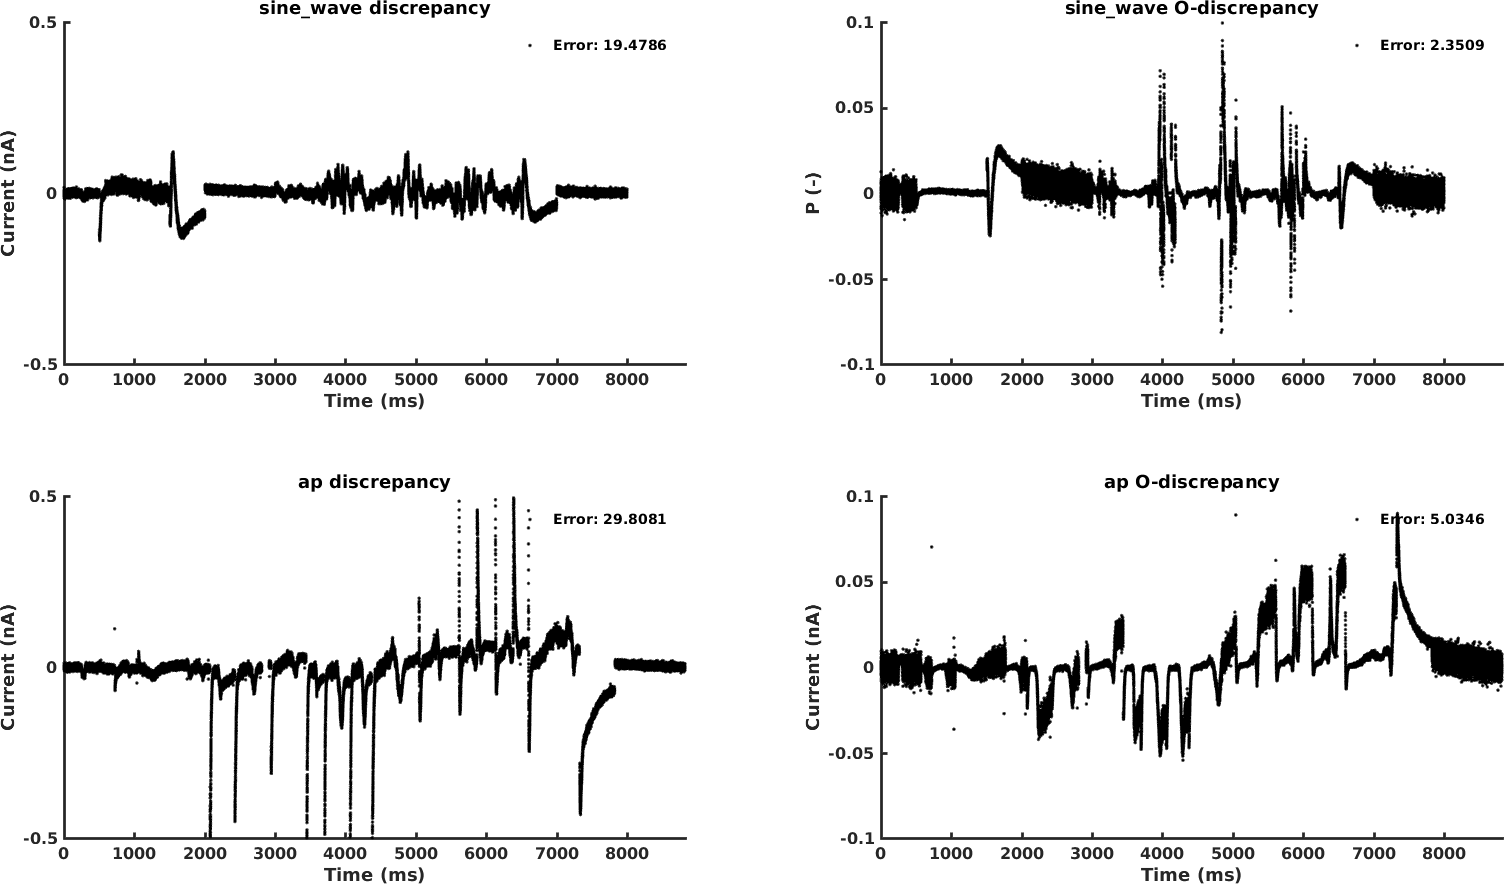
\includegraphics[scale=0.42]{Figures/PlotDiscrepancyVsDiscrepancyInOpen_sine_wave_ap.png}
\caption{\textbf{Discrepancies for the sine wave (top) and action potential (bottom) protocols.} The left hand column shows $d$ and the right hand column shows $d_o$. Capacitative spikes have been removed.}
\label{Fig_Discrepancy}
\end{center}
\end{figure}


\subsection{Structural discrepancy}
Both of the above definitions rely on a particular parameterisation of the model. However, it is also possible to consider the model discrepancy as being the difference between the model and reality. This concept is explained in more detail in \cite{Kennedy2002} and \cite{Strong2014} and refers to the structure of the model rather than its parameterisation.  This definition of model discrepancy refers to model structure, rather than model parameterization (which would change $d$ and $d_o$, above). In the context of hERG modelling, this could be a relatively simple difference, such as the number of closed states in a model or the form of the rate constants. Alternatively, it could be an entirely different feature not preserved in the model of interest - consider the difference between a molecular dynamics simulation of channel opening and a four state Markov model. In this project, we considered this form of discrepancy by fitting four models to the same data and then exploring how their evolution differed in time (Section \ref{Sec_ModelDiscrepancy}).

\section{Statistical Prediction of Discrepancy}

\subsection{Introduction}

Our goal was to predict simulation discrepancy when using fitted models for prediction. The goal would then be to quantify, based on the training data and the prediction simulation, where and by how much the prediction simulation would differ from the actual experimental trace recorded from that cell, for the prediction protocol. In this report, we use two methods, LASSO and the Matlab method Stepwise Linear Model.

\subsection{Input Variables}\label{SubSec_Predictors}

As an initial hypothesis, we proposed to use properties derivable from the model equations shown in Eqs.~\eqref{Eq_dCdt}-\eqref{Eq_I_hh}. These properties are
\begin{itemize}
\item Variables $y_1$, $y_2$, $y_3$, $y_4$.
\item Rates $K_{ij}$
\item Fluxes $y_i K_{ij}$
\item Current $I$
\item Voltage $V$
\item Voltage time derivative $\frac{dV}{dt}$
\item Time $t$
\item Parameter sensitivities $\frac{dy_i}{dp_j}$
\item Current sensitivity $\frac{dI}{dp_j} = G \frac{dy_3}{dp_j} (V-V_E) $
\end{itemize}

Parameter sensitivities are derived using the following equation \cite{}. Using $s_{ij} = \frac{dy_i}{dp_j}$,
\begin{align}
	\frac{\partial}{\partial p_j} ( \frac{dy_i}{dt} ) & = \frac{\partial}{\partial p_j} (f( y ) ) \\
	\frac{d}{dt}(\frac{\partial y_i}{\partial p_j})   & = \frac{\partial f}{ \partial y_i}\frac{\partial y_i}{ \partial p_j} + \frac{\partial f}{ \partial p_j} \\
	\frac{d s_{ij}}{dt} & = \frac{\partial f}{ \partial y_i} s_{ij} + \frac{\partial f}{ \partial p_j}
\end{align}
The CVODES libraries are used to integrate the parameter sensitivity equations alongside the ODEs in Eqns.~\eqref{Eq_dCdt}-\eqref{Eq_I_hh}.

Before performing any estimation, we check for linear dependence of each set of properties in turn, then check for linear dependence of all the properties that remain. The linear independence check is numerical and performed using the Mathworks File Exchange program getLinearDependent.m. Note that we did not include the derivatives of the variables ($\frac{dy_i}{dt}$) because they are linear combinations of the fluxes.

\subsection{Experimental Data}
For the purposes of this study we restricted ourselves to one cell from the study by \cite{}, the `middle' cell in terms of quality that is used in most of the plots in that paper. This cell has cell identifier 16713110. A number of experimental voltage protocols are used in this study. The main focus is on the `sine wave' (SW) and `action potential' (AP) protocols used by Beattie \textit{et al}\cite{Beattie2018}. However, we also used some other protocols recorded during data collection for this study, namely the `Original Sine Wave' (OSW), `Equal Proportions' (EP), and `Mazahari-Wang Difference' (MWDD) protocols. All protocols used and the corresponding experimentally recorded current are shown in Fig.~\ref{Fig_Protocols}. For the purposes of fitting, all capacitance spikes were removed as in Beattie \textit{et al}\cite{Beattie2018}.

\begin{figure}[t]
\begin{center}
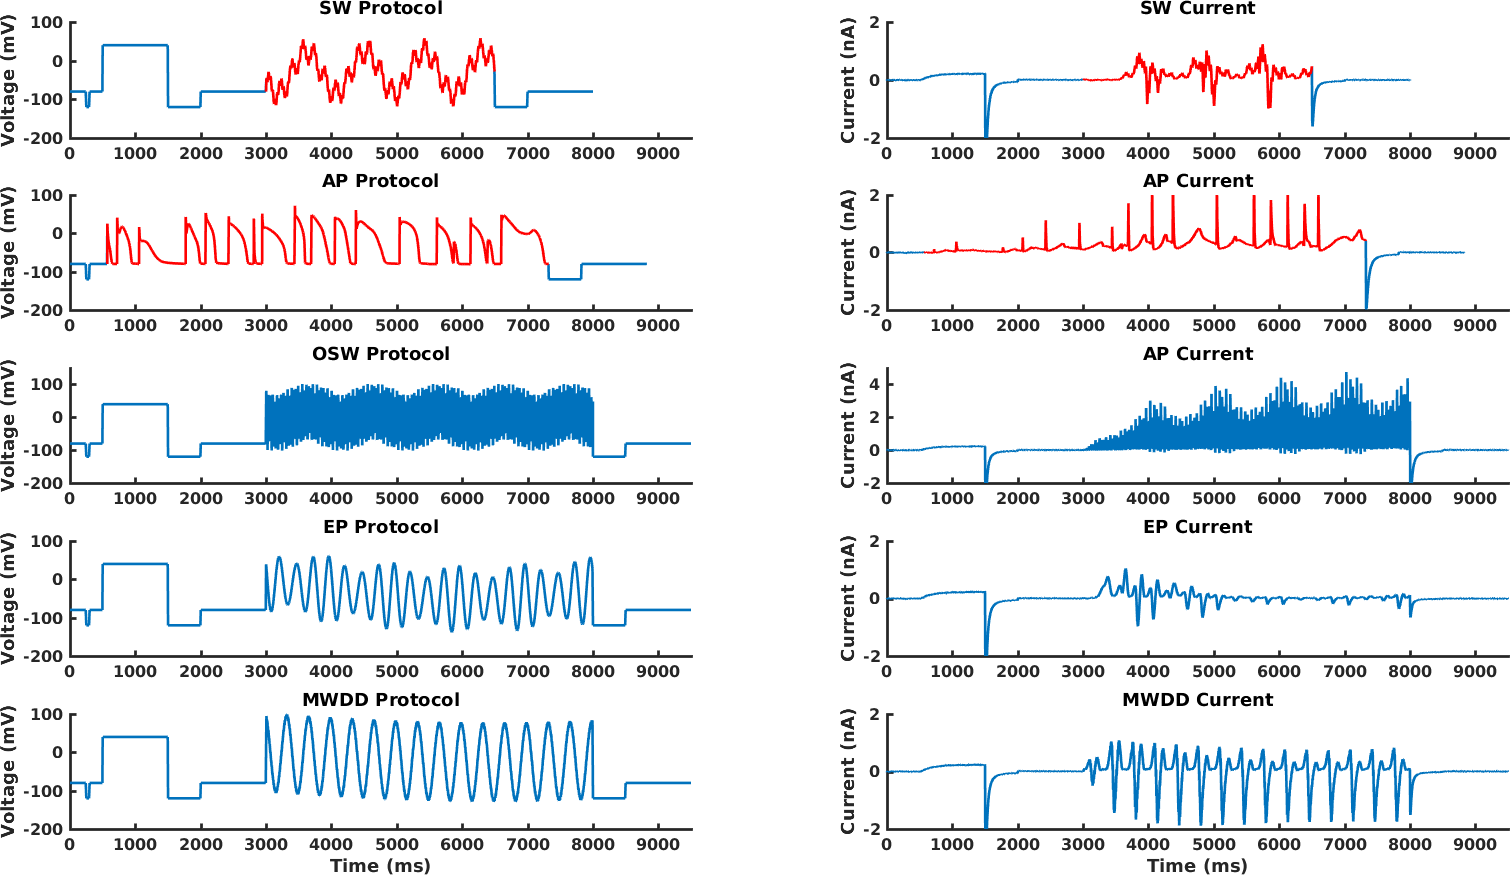
\includegraphics[scale=0.42]{Figures/Protocols.png}
\caption{\textbf{Protocols and current traces used in this report.} All five protocols and the resulting current traces for cell 16713110 as used in this study are shown with capacitative spikes removed. For the SW and AP protocols, the `core' of the protocol used in Sections \ref{SubSec_Lasso_Discrepancy} and \ref{SubSec_StepwiseLM_Discrepancy} are highlighted in red. Note that the y-axis scale for the OSW protocol and current differ from the other protocols due to the higher (and non-physiological) potentials reached - this was one reason for the rejection of the OSW protocol during the development of the SW protocol.}
\label{Fig_Protocols}
\end{center}
\end{figure}

\subsection{Predicting Discrepancy Using LASSO}\label{SubSec_Lasso_Discrepancy}

\subsubsection{The Method}
The Least Absolute Shrinkage and Selection Operator (LASSO)\footnote{\url{https://www.mathworks.com/help/stats/lasso.html}} is a popular linear regression method that incorporates a regularization parameter $\lambda$. For a set of predictors $X$, $N$ data points $y$ and coefficients $\beta$, the LASSO method can be written in Lagrangian form as
\begin{align}
	\min_{\beta} ( \frac{1}{N} \norm{ y - \beta X }^2 + \lambda \norm{ \beta }^1 ).
\end{align}
The size of the parameter $\lambda$ determines the degree of regularization. Essentially, a large $\lambda$ penalizes $\beta$ heavily, and so produces smaller models. Conversely, a small $\lambda$ allows the method more freedom in the number of variables included. A key feature of the LASSO algorithm is that due to the $L_1$ norm used for regularization, elements of $\beta$ can be set to zero by the method, resulting in smaller models. This key property has made LASSO a popular method in Machine Learning. Variations on this method are Ridge regression (uses $\lambda \norm{ \beta }^2$ instead) and Elastic Net regression (a combination of Ridge and LASSO).

One challenge of the LASSO method is that there is no a priori choice for the regularization parameter $\lambda$. To determine $\lambda$ and check the validity of the resulting models we use K-fold cross-validation. This method works by splitting the experimental data into K equally sized folds, leaving one out, then checking the model's ability to predict the data in the left out fold. This results in a mean squared error (MSE) for each fold, and for each value of $\lambda$. The variation in the MSE at each $lambda$ can be used to select $\lambda$ and hence, the model. To do so, we find the $\lambda$ value giving the minimum MSE, and then choose the largest $\lambda$ within one standard deviation from this point. This can be seen as choosing the smallest justifiable  model within the variation of the model that gives the absolute minium error. In this study, we use 10 folds which is a fairly standard choice.

An important property of K-fold cross-validation as inplemented in Matlab is that it uses random data points in each fold. While this is in principle a good thing, the extremely high time resolution of our data means that all of the resulting folds are likely to be effectively the same, subject to experimental noise. As a result, the models produced by the Matlab algorithm were both non-predictive and non-deterministic. To correct for this phenomenon and produce meaningful folds, some editing of the Matlab source code is required (detailed in README.md). We instead split the trace into ten equal segments consecutive in time to ensure variation between folds.

\subsubsection{Results}

LASSO fits for a linear regression model of model discrepancy of $d$ and $d_o$ are shown in Figure \ref{Fig_LASSO_SW_AP_full_discrepancy}. For this model, the discrepancies resulting from the sine wave (SW) protocol developed in by Beattie et al.~was used as training data, and was used to predict the results from the action potential (AP) protocol used for validation in that study. The resulting corrected currents together with the original simulation and experimental data are shown in Fig.~\ref{Fig_LASSO_SW_AP_full_currents}. It can be appreciated that, in both cases, the linear models of discrepancy fail to predict the discrepancy observed in the AP trace.

\begin{figure}[t]
\begin{center}
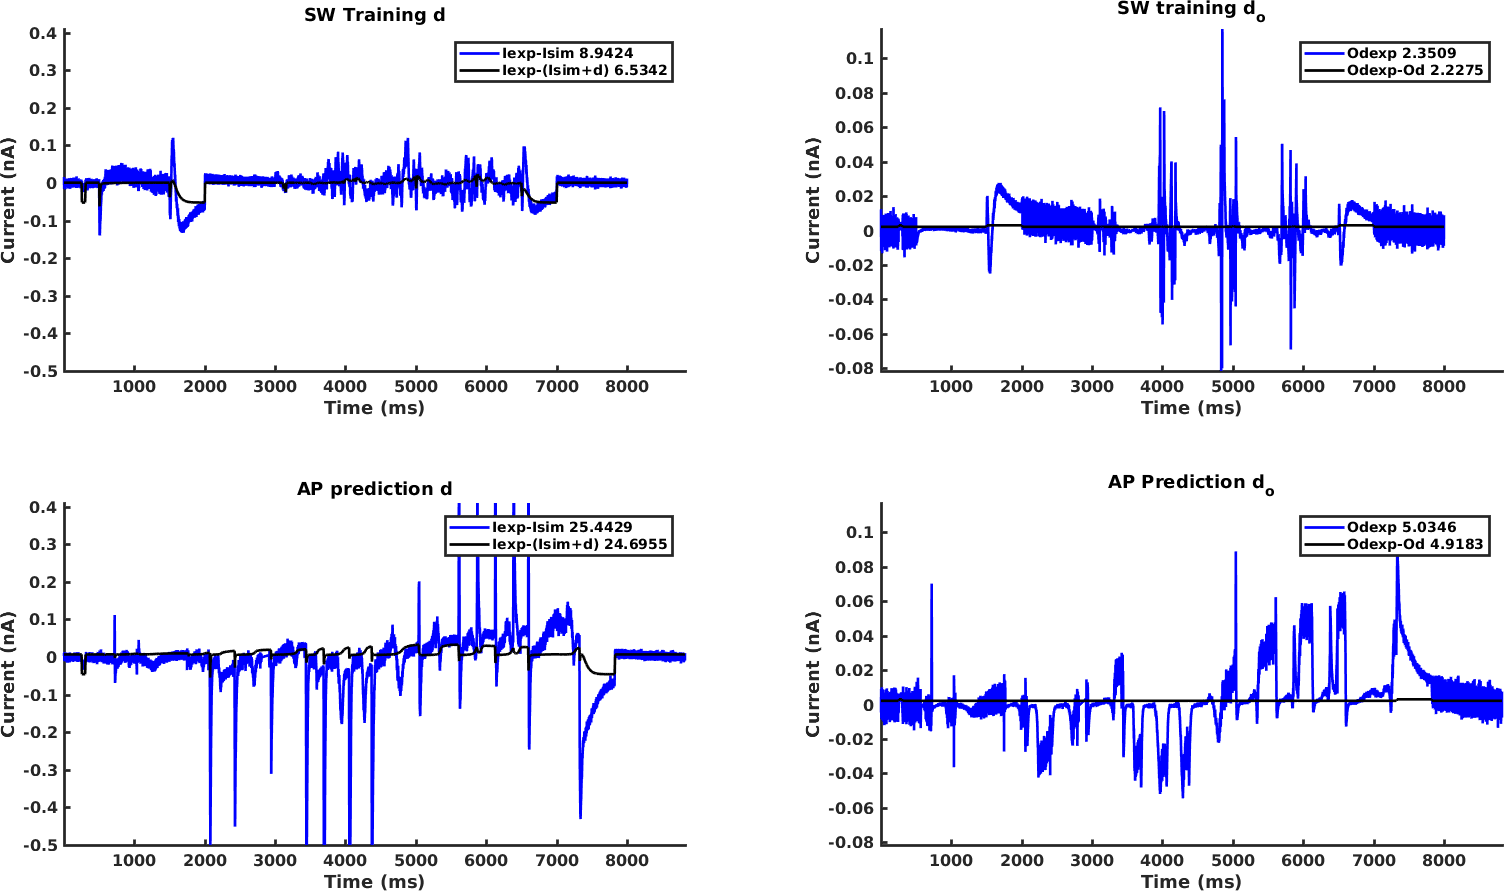
\includegraphics[scale=0.42]{Figures/LASSO_SW_AP_full_discrepancy.png}
\caption{\textbf{Linear model of discrepancy constructed using LASSO from the SW protocol.} These models of $d$ (left) and $d_o$ (right) were constructed using LASSO on the entire SW trace (top), starting with all linearly independent predictors. The improvement of the training trace (top) is poor and the resulting models fail to predict the discrepancy in the AP trace (bottom). The root mean square errors between the simulated and predicted traces are shown in the legends. } 
\label{Fig_LASSO_SW_AP_full_discrepancy}
\end{center}
\end{figure}

\begin{figure}[hb]
\begin{center}
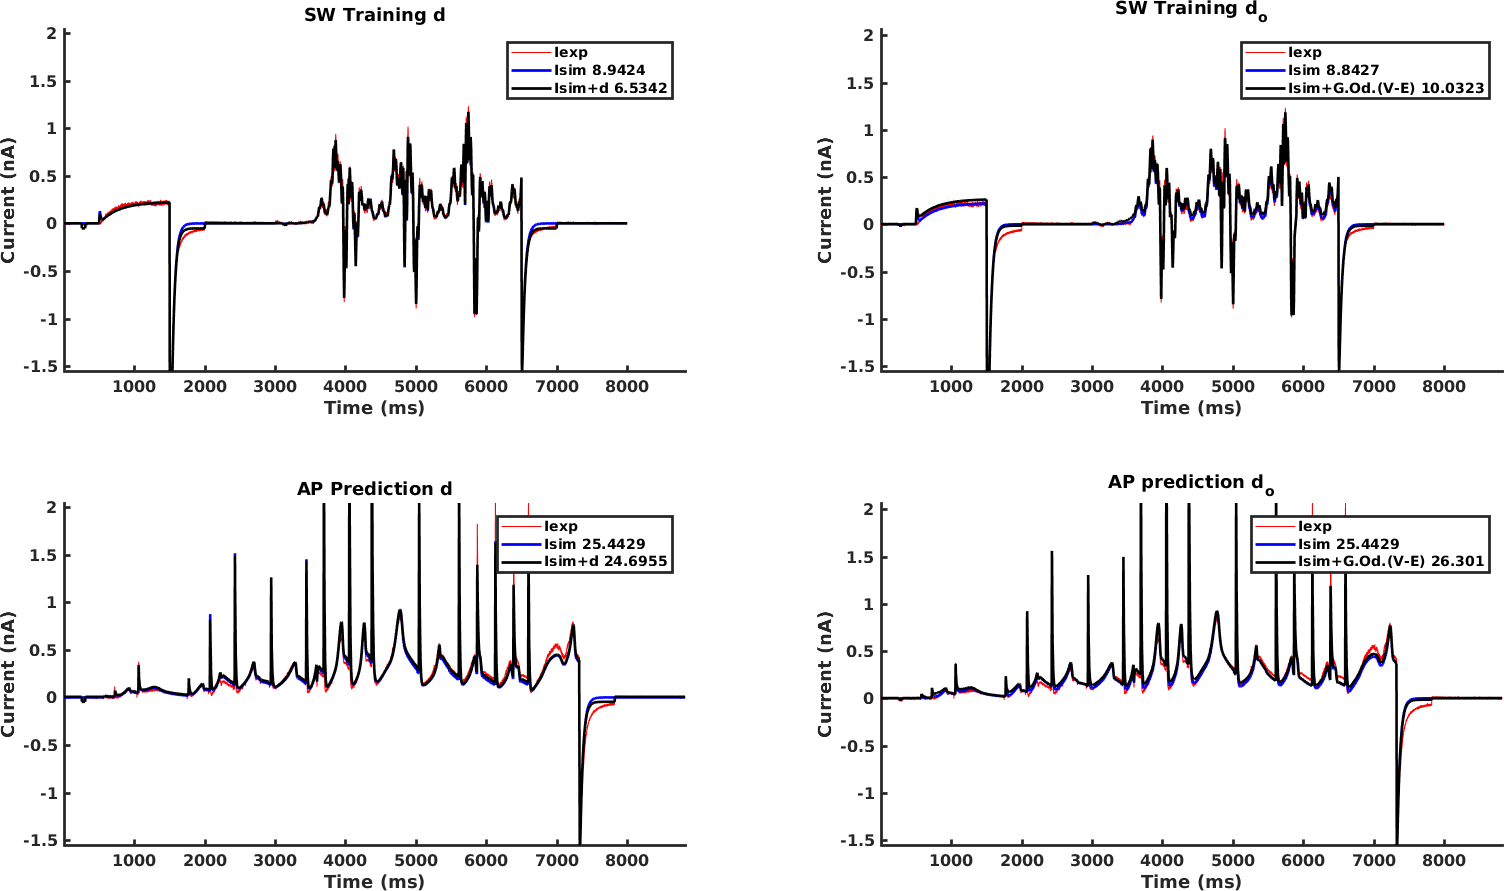
\includegraphics[scale=0.42]{Figures/LASSO_SW_AP_full_currents.png}
\caption{\textbf{Corrected currents using a linear model of discrepancy constructed using LASSO from the SW protocol.} The models of $d$ (left) and $d_o$ (right) in Fig. ~\ref{Fig_LASSO_SW_AP_full_discrepancy} have been incorporated into the simulation (blue line), giving a revised prediction for the SW and AP protocols (black line). As expected from Fig.~\ref{Fig_LASSO_SW_AP_full_discrepancy}, there is little improvement in the agreement with the experimental data (red line). The sum of squared errors between the models and the data are shown in the legend.}
\label{Fig_LASSO_SW_AP_full_currents}
\end{center}
\end{figure}

Included parameters and their coefficients are shown in Fig.~\ref{Fig_LASSO_SW_AP_coefficients}. The parameters differ considerably between the models for $d$ and $d_o$. Fig.~\ref{Fig_LASSO_SW_AP_lambda} shows the plot of $\lambda$ as a function of MSE. The model with the minimum MSE is indicated by the green line and the model with the largest value of $\lambda$ (hence, the smallest model) within one standard error of the minimum MSE model is shown by the blue line. Note the characteristic U-shaped form of the $\lambda$ - MSE relationship, with overfitting on the right and underfitting on the left.

\begin{figure}[t]
\begin{center}
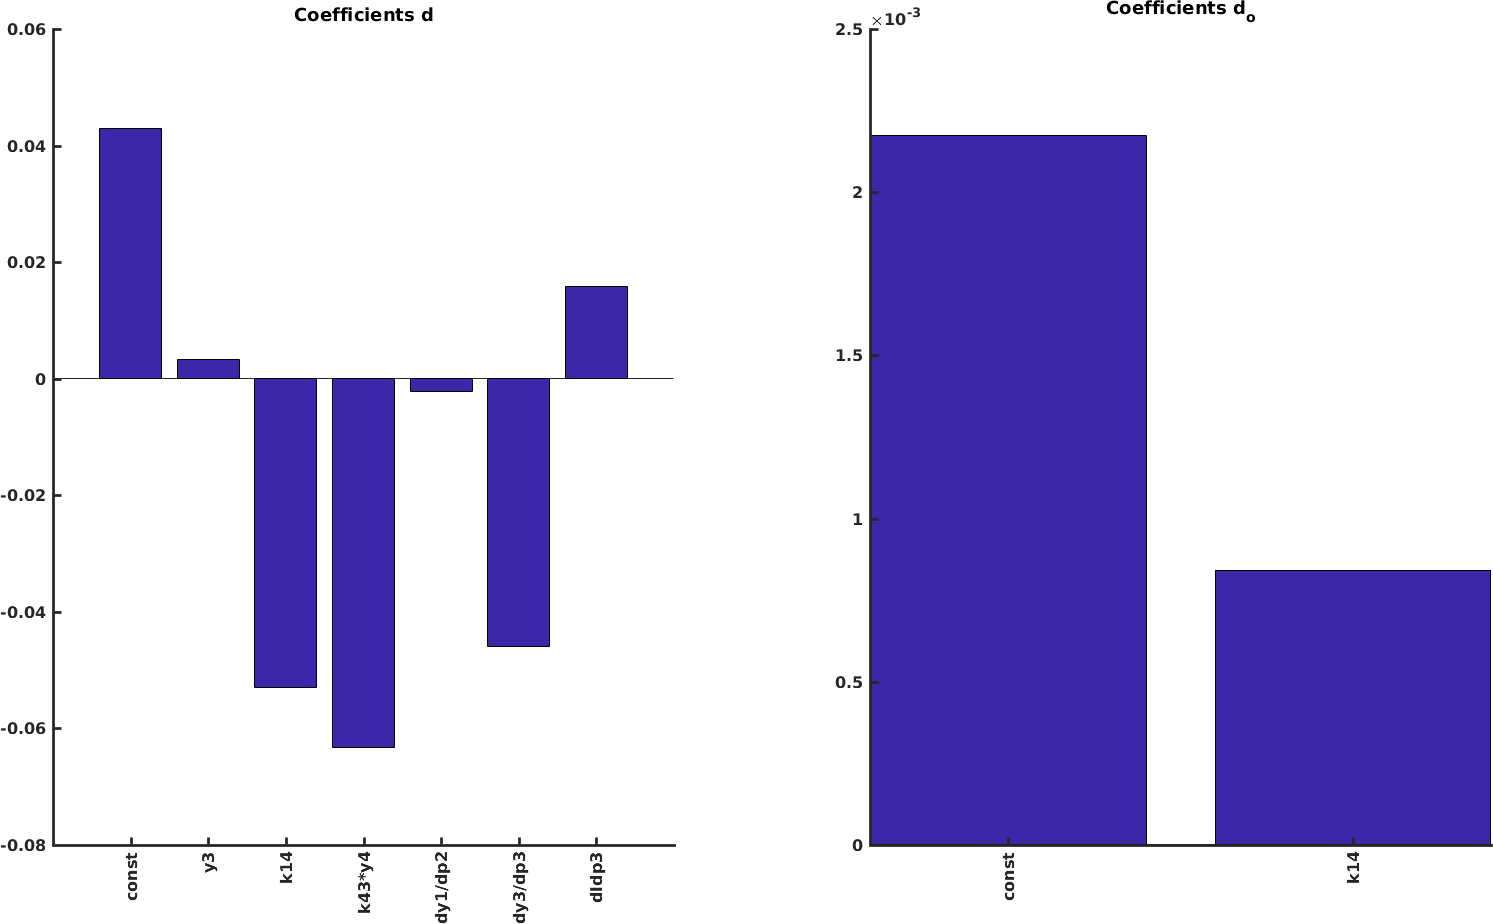
\includegraphics[scale=0.42]{Figures/LASSO_SW_AP_full_coefficients.png}
\caption{\textbf{Coefficients in the linear model of discrepancy constructed using LASSO from the SW protocol.} This plot shows the included parameters and coefficients for the model produced by LASSO shown in Fig.~\ref{Fig_LASSO_SW_AP_full_discrepancy} and Fig.~\ref{Fig_LASSO_SW_AP_full_currents}. Coefficients for $d$ are shown on the left, and coefficients for $d_o$ are shown on the right.} 
\label{Fig_LASSO_SW_AP_coefficients}
\end{center}
\end{figure}

\begin{figure}[hb]
\begin{center}
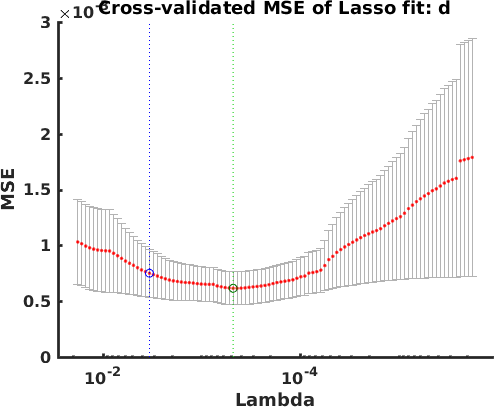
\includegraphics[scale=0.42]{Figures/LASSO_SW_AP_full_lambda_d.png}
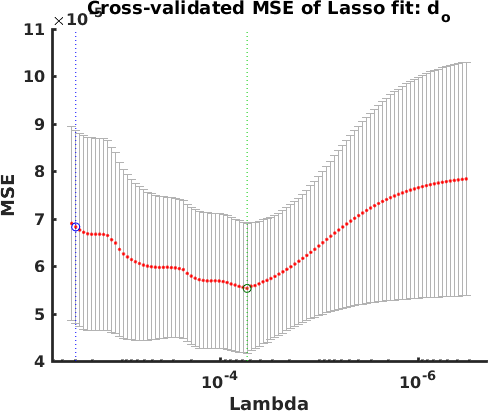
\includegraphics[scale=0.42]{Figures/LASSO_SW_AP_full_lambda_od.png}
\caption{\textbf{$\lambda$ and Mean Squared Error plots from the linear models of the SW protocol.} The models of $d$ (left) and $d_o$ (right) have been generated by varying $\lambda$. The error bars indicate the standard error in the MSE between folds. The value of $\lambda$ giving the minimum MSE is indicated by the green line and the selected value of $\lambda$, being the largest value of $\lambda$ with an MSE within one standard error of the minimum, is shown in blue. Note that $\lambda$ runs from largest to smallest, so that the largest model is on the left.}
\label{Fig_LASSO_SW_AP_lambda}
\end{center}
\end{figure}

\clearpage

Based on the failure of the `naive' LASSO method in this standard case, we also addressed the following hypotheses:
\begin{itemize}
\item the LASSO method might be biased by the large errors that occur in the deactivation steps, and so fail to fit the more subtle errors in the main part of the trace.
\item Because the fit to the SW protocol is `optimal' and  extremely good, there may simply not be enough information in the discrepancy of the sine wave protocol to train a model.
\end{itemize}

To address the first hypothesis, we tried fitting a model to only the sine wave generated part of the SW protocol, and omit the activation and deactivation steps on either end (see Fig.~\ref{Fig_Protocols}). These were then used to predict only the section of the AP protocol containing the action potentials. To address the second hypothesis, we instead trained the models using alternative protocols (OSW, EP, MWDD) that were recorded during the course of the sine wave protocol study. Results for each of these approaches are shown in Fig.~\ref{Fig_LASSO_SW_AP_core_discrepancy}-\ref{Fig_LASSO_AP_AP_full_lambda}. In each case, the linear model of discrepancy only provides marginal gains in the training data, and either fails to improve the discrepancy in the prediction (AP) trace or makes it worse. In general, across all sets of results, the discrepancy in the open probability, $d_o$, appears to be both harder to predict and lead to more over-fitting than the standard definition, $d$.

To investigate what the `best possible' model would look like, we also constructed a model from our prediction data, namely the discrepancy in the AP protocol. The quality of this fit effectively places an upper bound on the success of the LASSO procedure for constructing a linear model of the data we wish to predict. This model is shown in Figs.~\ref{Fig_LASSO_SW_AP_core_discrepancy}-\ref{Fig_LASSO_OSW_AP_core_lambda}. Whilst this model produces an appreciable improvement in the agreement between data and model, this result suggests that a linear regression approach would only ever be able to account for a sub-portion of the discrepancy observed between simulation and experiment.

\begin{figure}[t]
\begin{center}
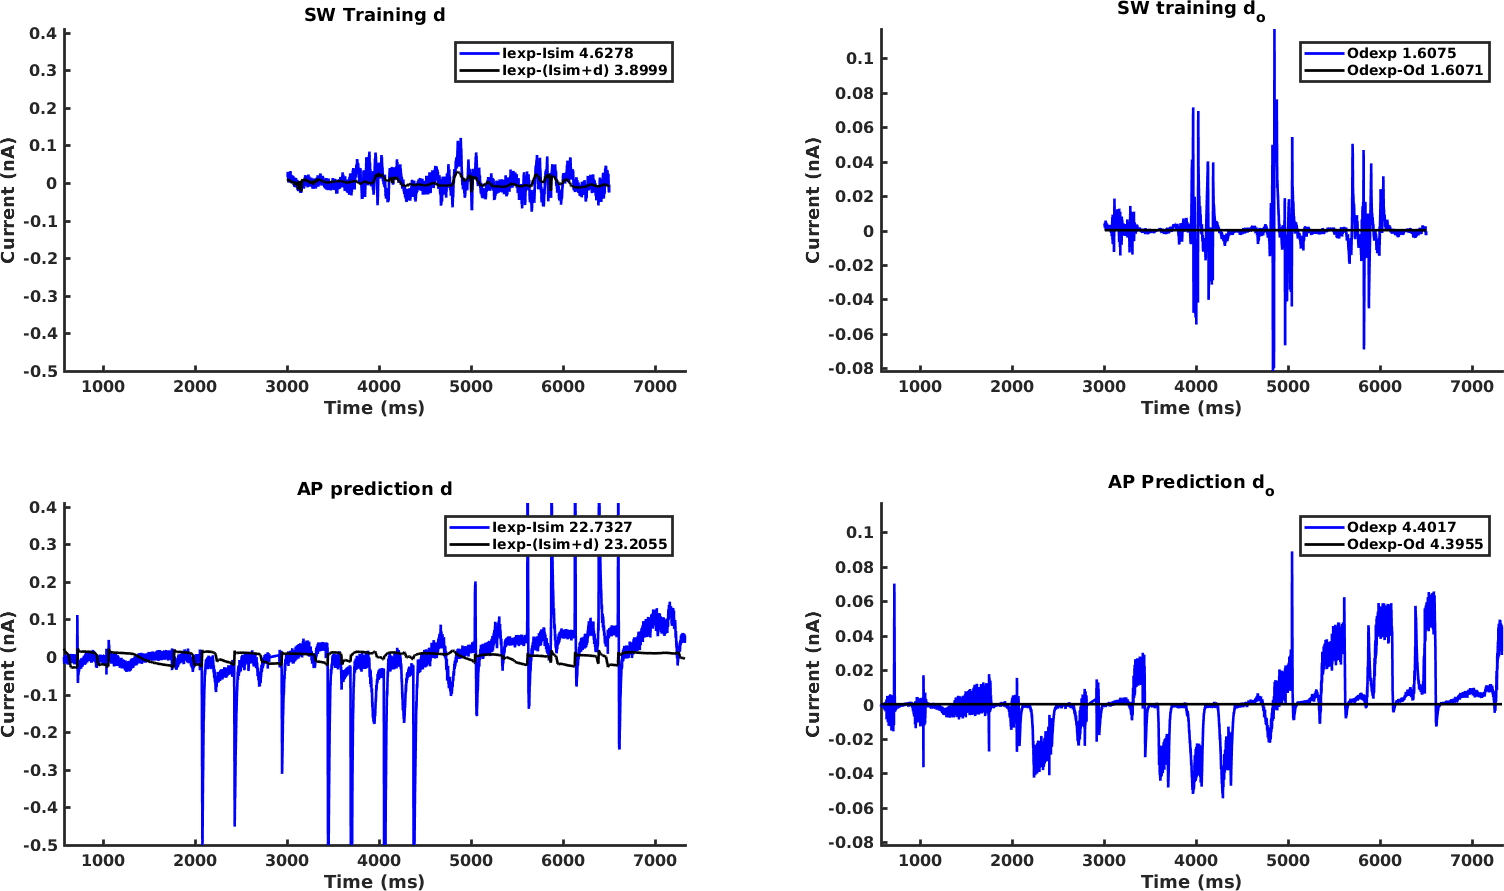
\includegraphics[scale=0.42]{Figures/LASSO_SW_AP_core_discrepancy.png}
\caption{\textbf{Linear model of discrepancy constructed using LASSO.} These models of $d$ (left) and $d_o$ (right) were constructed using LASSO on the entire SW trace (top), starting with all linearly independent predictors. The root mean square errors between the simulated and predicted traces are shown in the legends. } 
\label{Fig_LASSO_SW_AP_core_discrepancy}
\end{center}
\end{figure}

\begin{figure}[hb]
\begin{center}
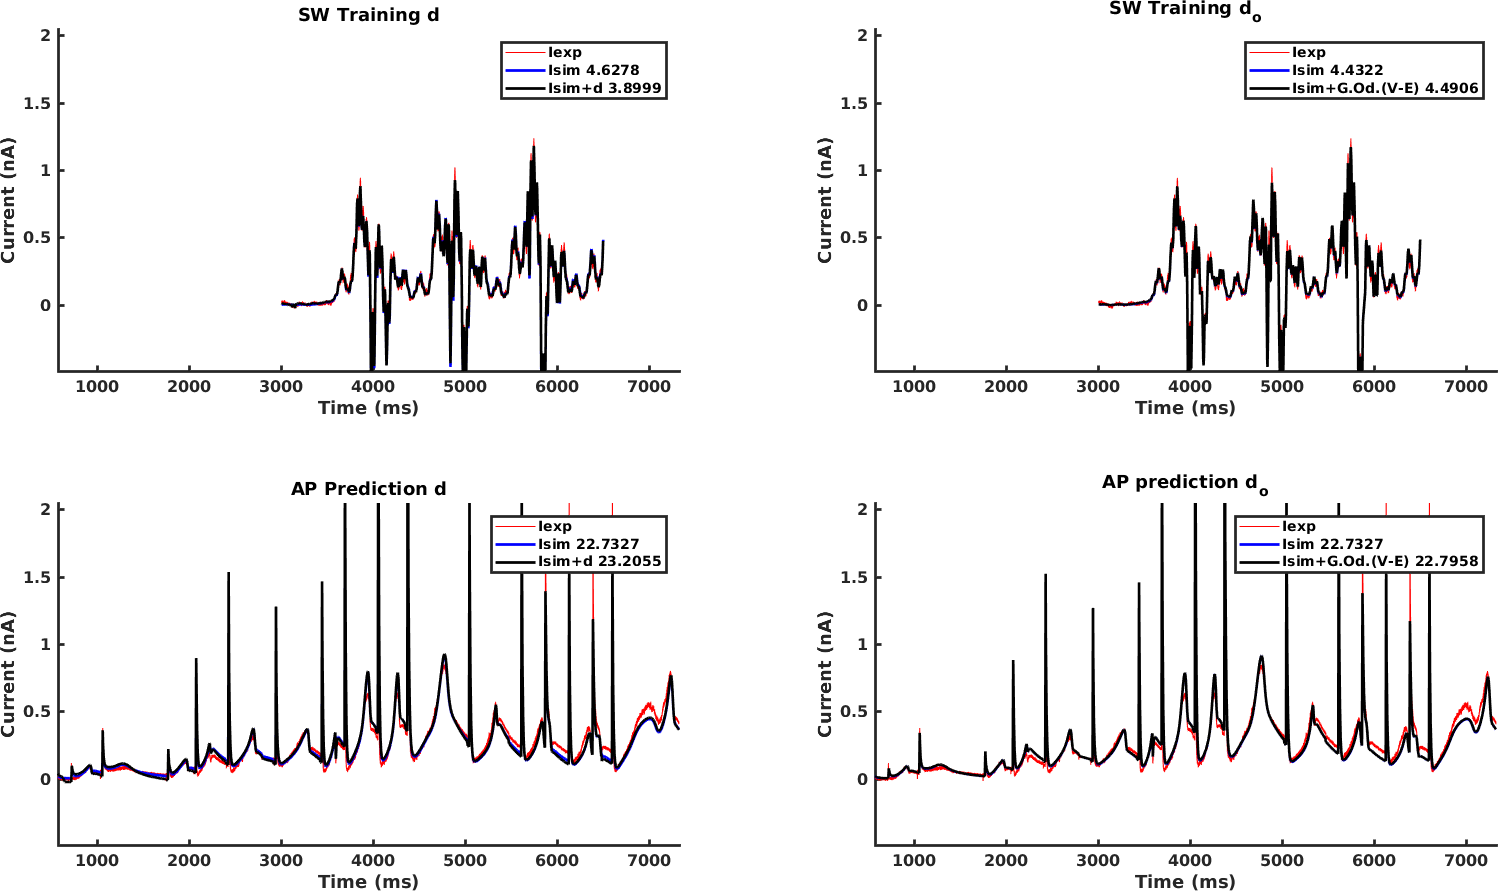
\includegraphics[scale=0.42]{Figures/LASSO_SW_AP_core_currents.png}
\caption{\textbf{Corrected currents using a linear model of discrepancy constructed using LASSO from the sine wave generated component of the SW protocol.} The models of $d$ (left) and $d_o$ (right) in Fig.~\ref{Fig_LASSO_SW_AP_core_discrepancy} have been incorporated into the simulation (blue line), giving a revised prediction for the SW and AP protocols (black line). The sum of squared errors between the models and the data are shown in the legend.}
\label{Fig_LASSO_SW_AP_core_currents}
\end{center}
\end{figure}

\clearpage

\begin{figure}[t]
\begin{center}
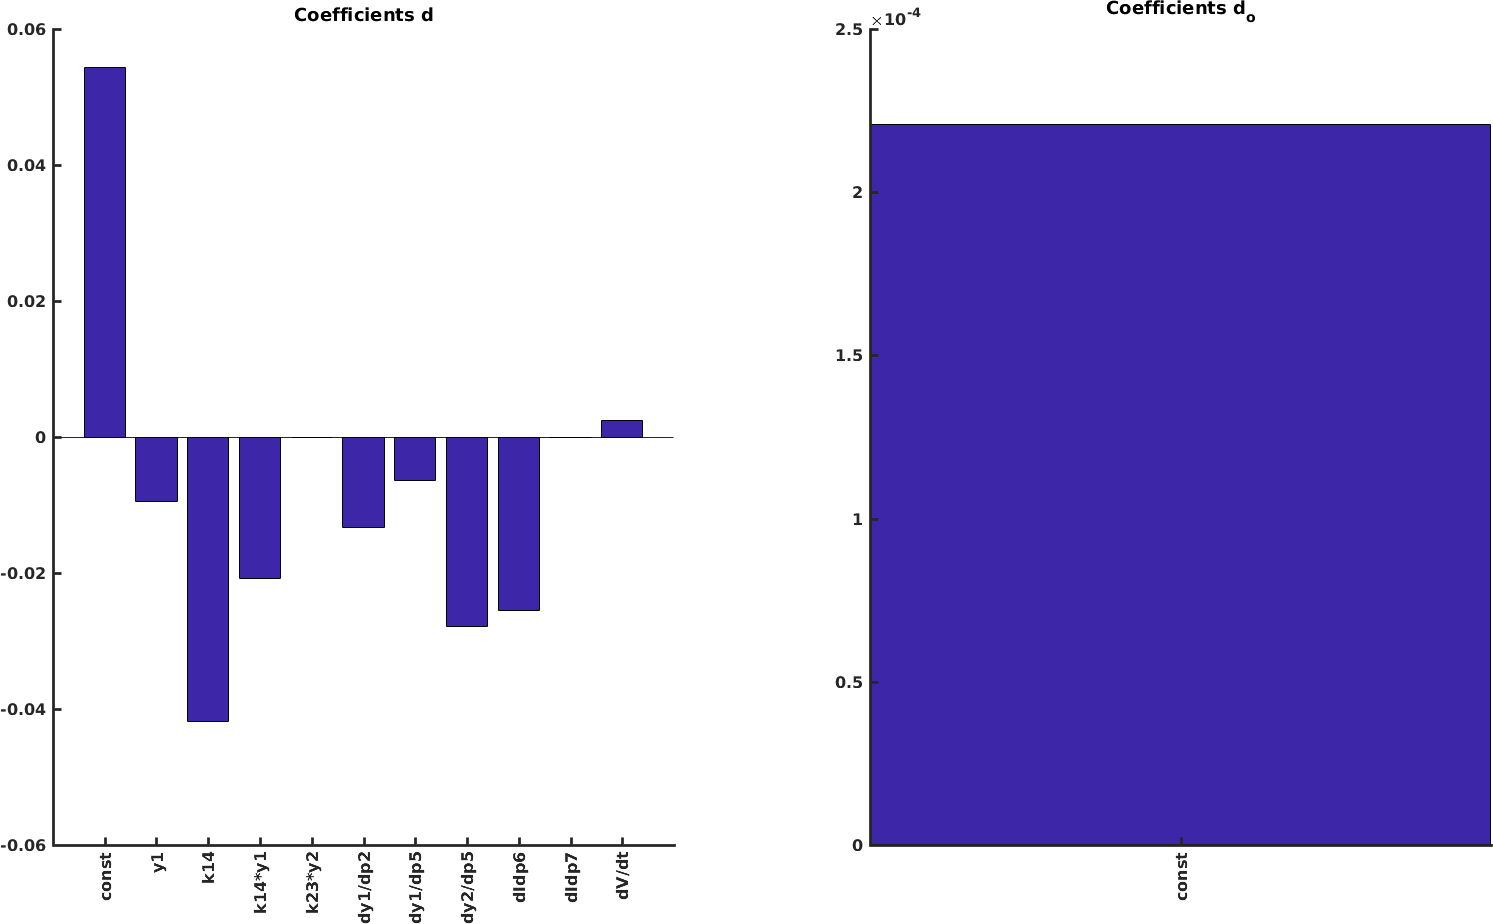
\includegraphics[scale=0.42]{Figures/LASSO_SW_AP_core_coefficients.png}
\caption{\textbf{Coefficients in the linear model of discrepancy constructed using LASSO from the sine wave generated component of the SW protocol.} This plot shows the included parameters and coefficients for the model produced by LASSO shown in Fig.~\ref{Fig_LASSO_SW_AP_core_discrepancy} and Fig.~\ref{Fig_LASSO_SW_AP_core_currents}. Coefficients for $d$ are shown on the left, and coefficients for $d_o$ are shown on the right.} 
\label{Fig_LASSO_SW_AP_core_coefficients}
\end{center}
\end{figure}

\begin{figure}[hb]
\begin{center}
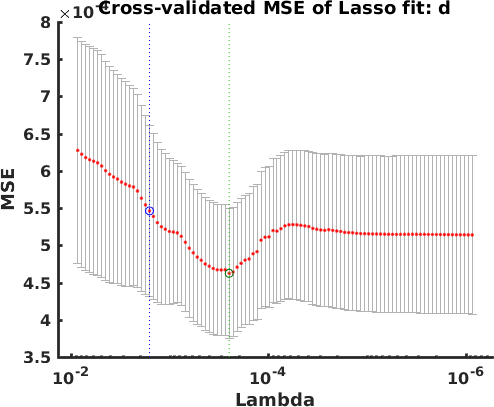
\includegraphics[scale=0.42]{Figures/LASSO_SW_AP_core_lambda_d.png}
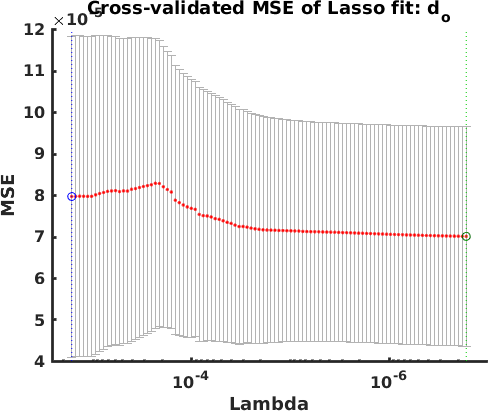
\includegraphics[scale=0.42]{Figures/LASSO_SW_AP_core_lambda_od.png}
\caption{\textbf{$\lambda$ and Mean Squared Error plots from the linear models of the sine wave component of the SW protocol.} The models of $d$ (left) and $d_o$ (right) have been generated by varying $\lambda$. The error bars indicate the standard error in the MSE between folds. The value of $\lambda$ giving the minimum MSE is indicated by the green line and the selected value of $\lambda$, being the largest value of $\lambda$ with an MSE within one standard error of the minimum, is shown in blue. Note that $\lambda$ runs from largest to smallest, so that the largest model is on the left.}
\label{Fig_LASSO_SW_AP_core_lambda}
\end{center}
\end{figure}

\clearpage

\begin{figure}[t]
\begin{center}
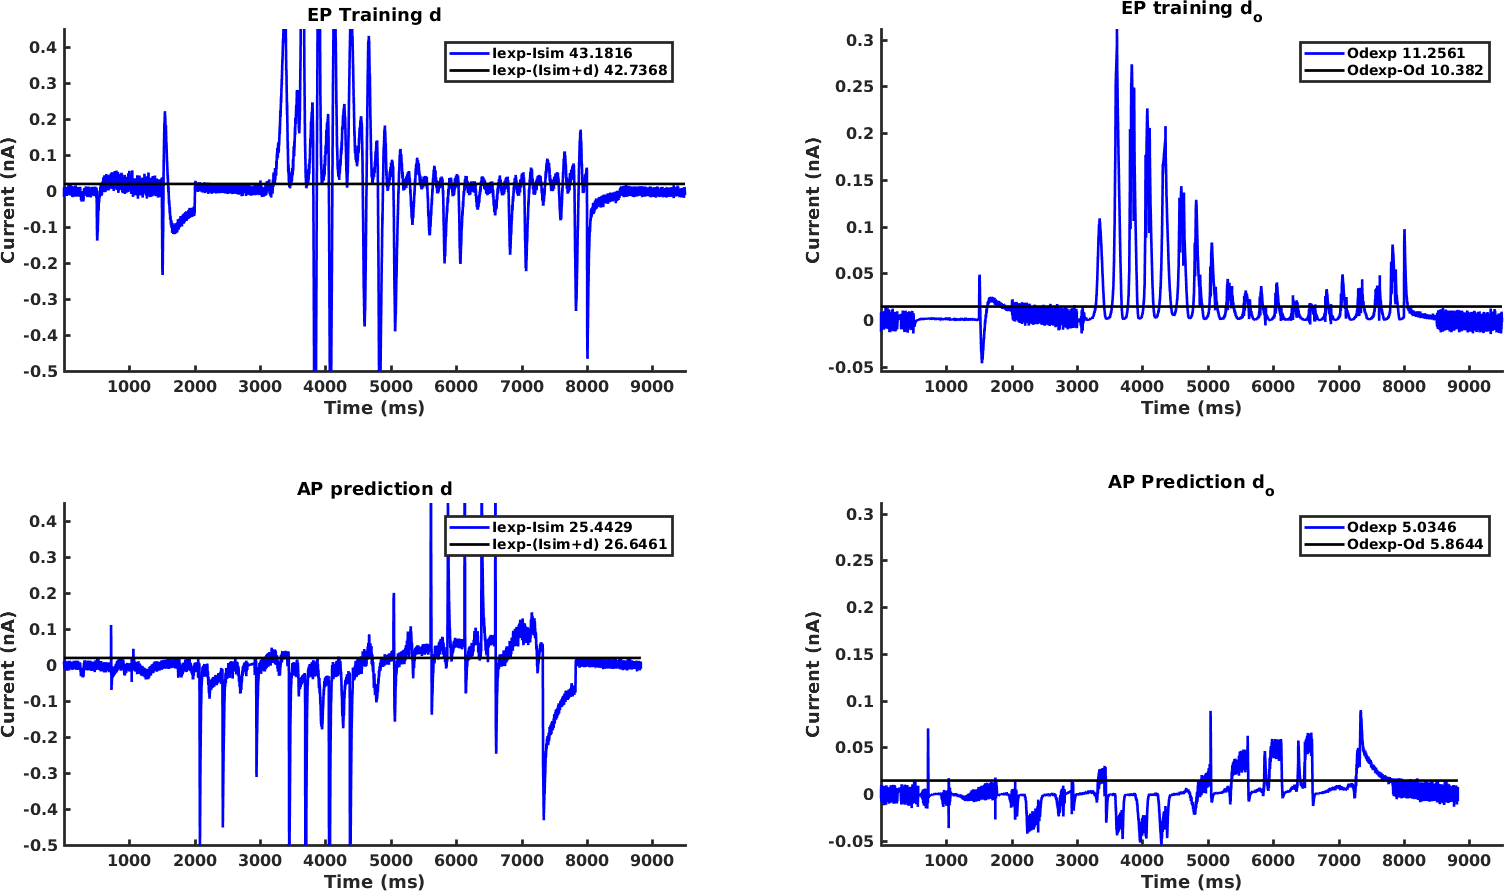
\includegraphics[scale=0.42]{Figures/LASSO_EP_AP_full_discrepancy.png}
\caption{\textbf{Linear model of discrepancy constructed using LASSO from the EP protocol.} These models of $d$ (left) and $d_o$ (right) were constructed using LASSO on the entire SW trace (top), starting with all linearly independent predictors. The root mean square errors between the simulated and predicted traces are shown in the legends. } 
\label{Fig_LASSO_EP_AP_full_discrepancy}
\end{center}
\end{figure}

\begin{figure}[hb]
\begin{center}
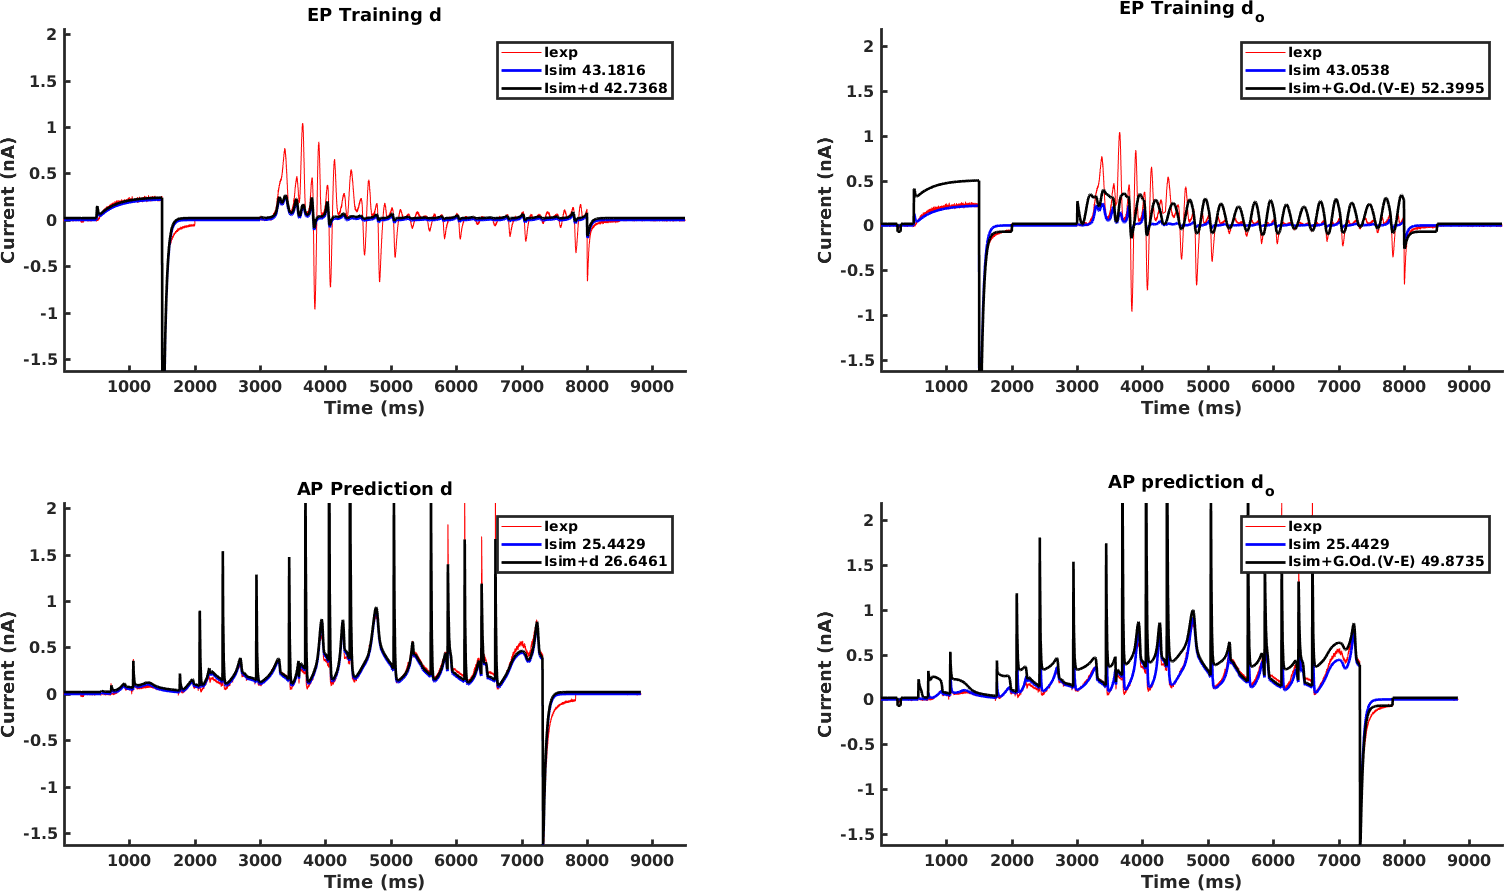
\includegraphics[scale=0.42]{Figures/LASSO_EP_AP_full_currents.png}
\caption{\textbf{Corrected currents using a linear model of discrepancy constructed using LASSO from the EP protocol.} The models of $d$ (left) and $d_o$ (right) in Fig. ~\ref{Fig_LASSO_SW_AP_full_discrepancy} have been incorporated into the simulation (blue line), giving a revised prediction for the EP and AP protocols (black line). The sum of squared errors between the models and the data are shown in the legend.}
\label{Fig_LASSO_EP_AP_full_currents}
\end{center}
\end{figure}

\clearpage

\begin{figure}[t]
\begin{center}
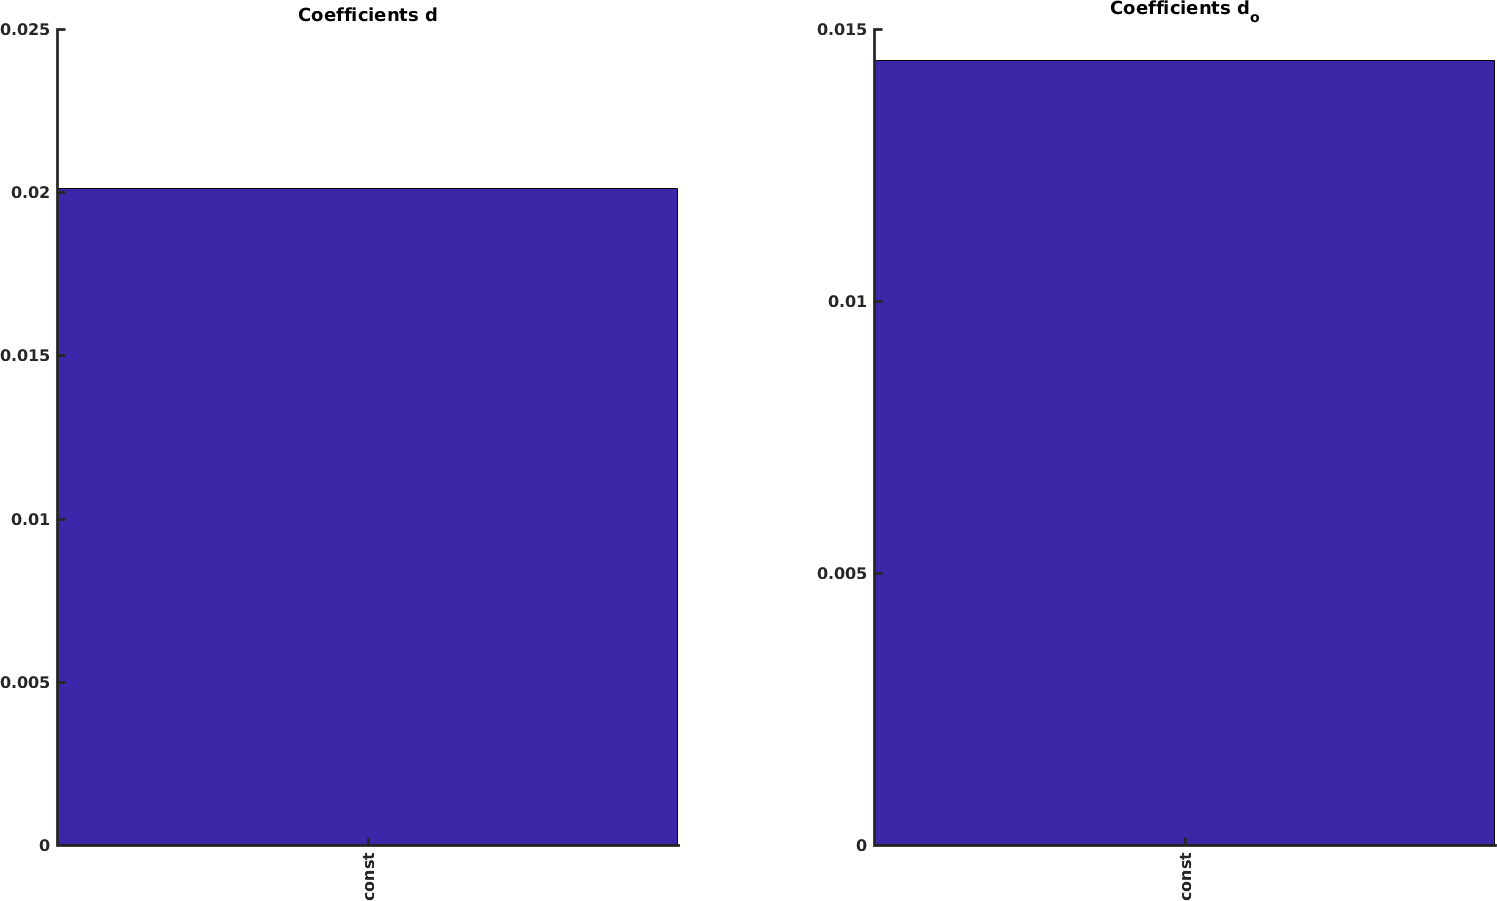
\includegraphics[scale=0.42]{Figures/LASSO_EP_AP_full_coefficients.png}
\caption{\textbf{Coefficients in the linear model of discrepancy constructed using LASSO from the sine wave generated component of the EP protocol.} This plot shows the included parameters and coefficients for the model produced by LASSO shown in Fig.~\ref{Fig_LASSO_EP_AP_full_discrepancy} and Fig.~\ref{Fig_LASSO_EP_AP_full_currents}. Coefficients for $d$ are shown on the left, and coefficients for $d_o$ are shown on the right.} 
\label{Fig_LASSO_EP_AP_full_coefficients}
\end{center}
\end{figure}

\begin{figure}[hb]
\begin{center}
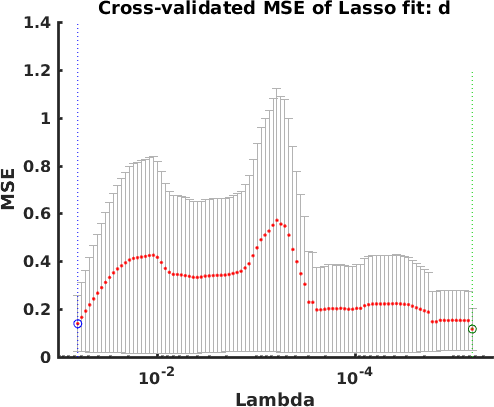
\includegraphics[scale=0.42]{Figures/LASSO_EP_AP_full_lambda_d.png}
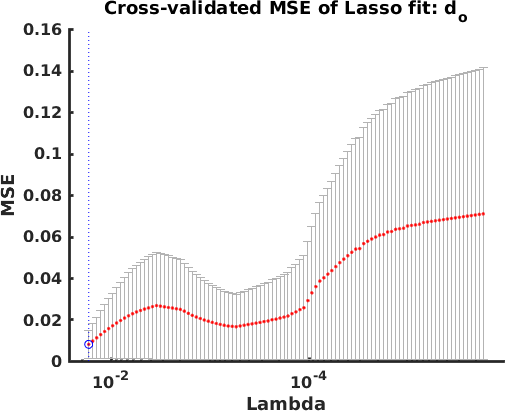
\includegraphics[scale=0.42]{Figures/LASSO_EP_AP_full_lambda_od.png}
\caption{\textbf{$\lambda$ and Mean Squared Error plots from the linear models of the sine wave component of the EP protocol.} The models of $d$ (left) and $d_o$ (right) have been generated by varying $\lambda$. The error bars indicate the standard error in the MSE between folds. The value of $\lambda$ giving the minimum MSE is indicated by the green line and the selected value of $\lambda$, being the largest value of $\lambda$ with an MSE within one standard error of the minimum, is shown in blue. Note that $\lambda$ runs from largest to smallest, so that the largest model is on the left.}
\label{Fig_LASSO_EP_AP_full_lambda}
\end{center}
\end{figure}

\clearpage

\begin{figure}[t]
\begin{center}
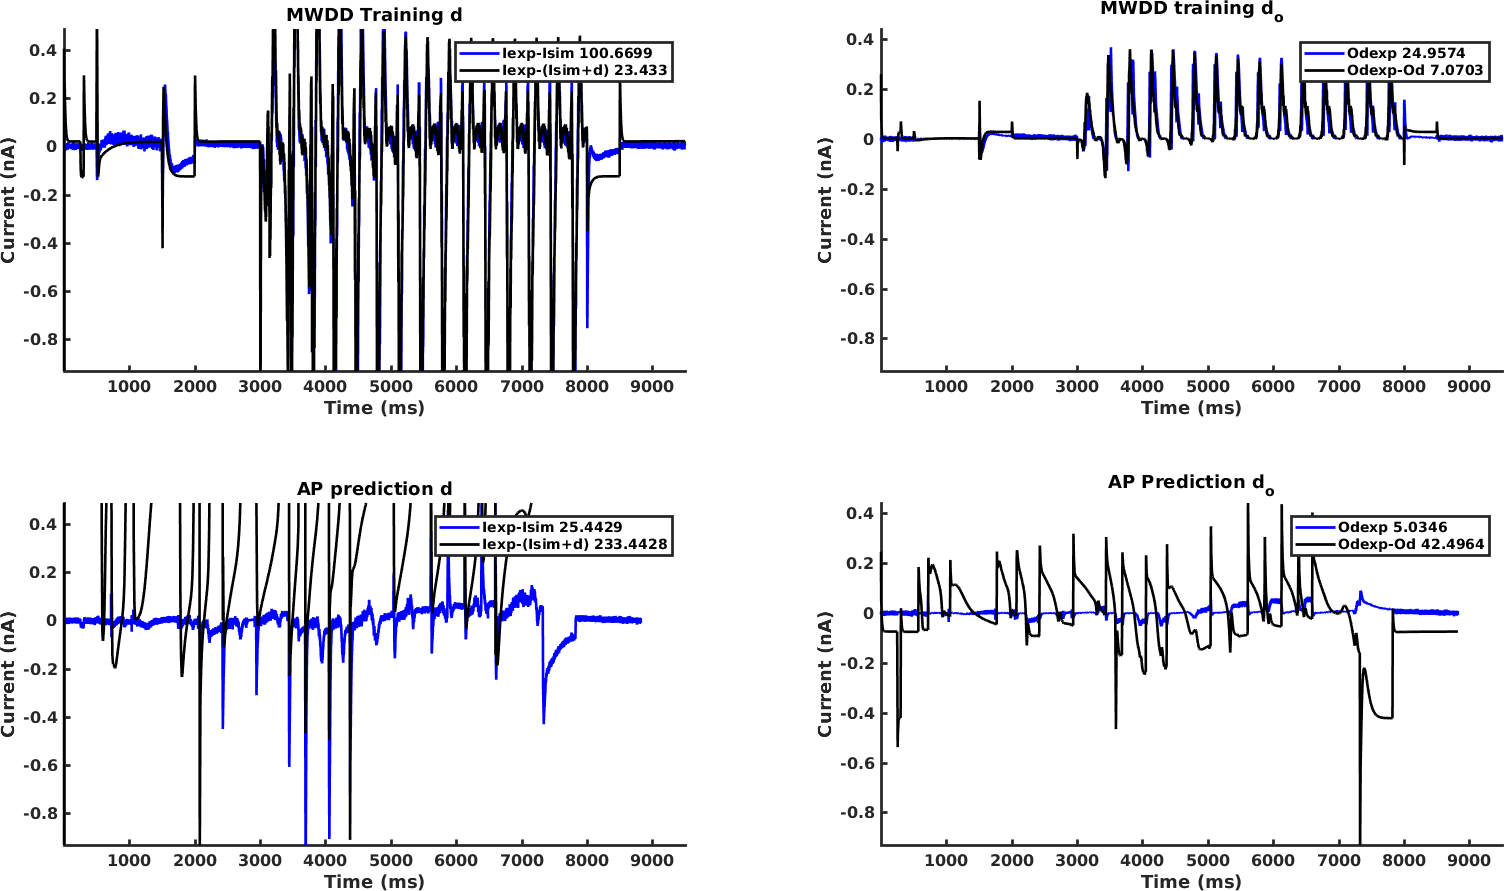
\includegraphics[scale=0.42]{Figures/LASSO_MWDD_AP_full_discrepancy.png}
\caption{\textbf{Linear model of discrepancy constructed using LASSO from the MWDD protocol.} These models of $d$ (left) and $d_o$ (right) were constructed using LASSO on the entire MWDD trace (top), starting with all linearly independent predictors. The root mean square errors between the simulated and predicted traces are shown in the legends. } 
\label{Fig_LASSO_MWDD_AP_full_discrepancy}
\end{center}
\end{figure}

\begin{figure}[hb]
\begin{center}
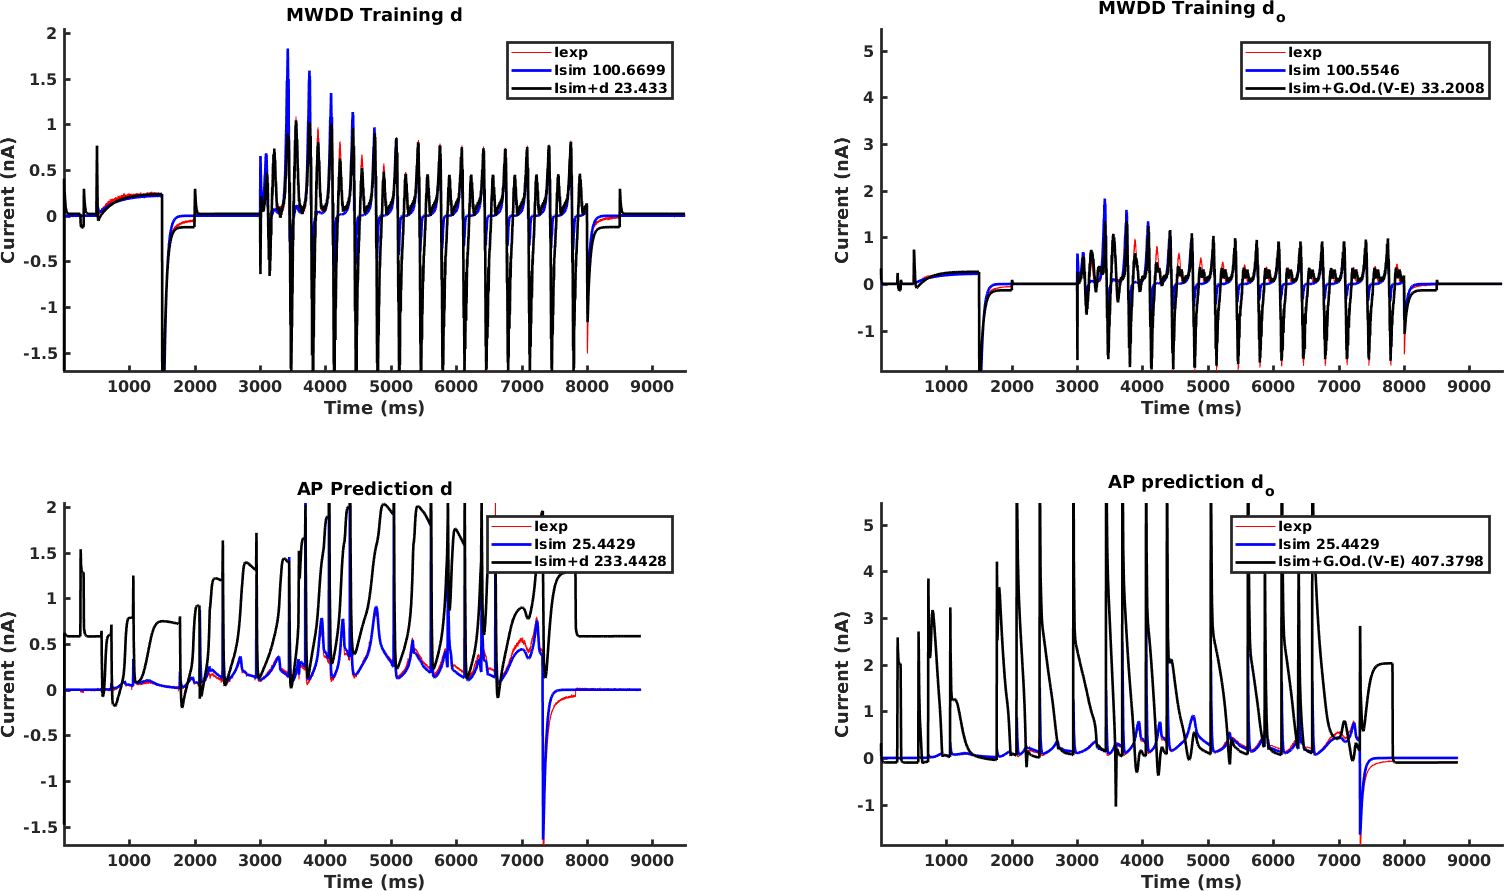
\includegraphics[scale=0.42]{Figures/LASSO_MWDD_AP_full_currents.png}
\caption{\textbf{Corrected currents using a linear model of discrepancy constructed using LASSO from the MWDD protocol.} The models of $d$ (left) and $d_o$ (right) in Fig. ~\ref{Fig_LASSO_MWDD_AP_full_discrepancy} have been incorporated into the simulation (blue line), giving a revised prediction for the MWDD and AP protocols (black line). The sum of squared errors between the models and the data are shown in the legend.}
\label{Fig_LASSO_MWDD_AP_full_currents}
\end{center}
\end{figure}

\clearpage

\begin{figure}[t]
\begin{center}
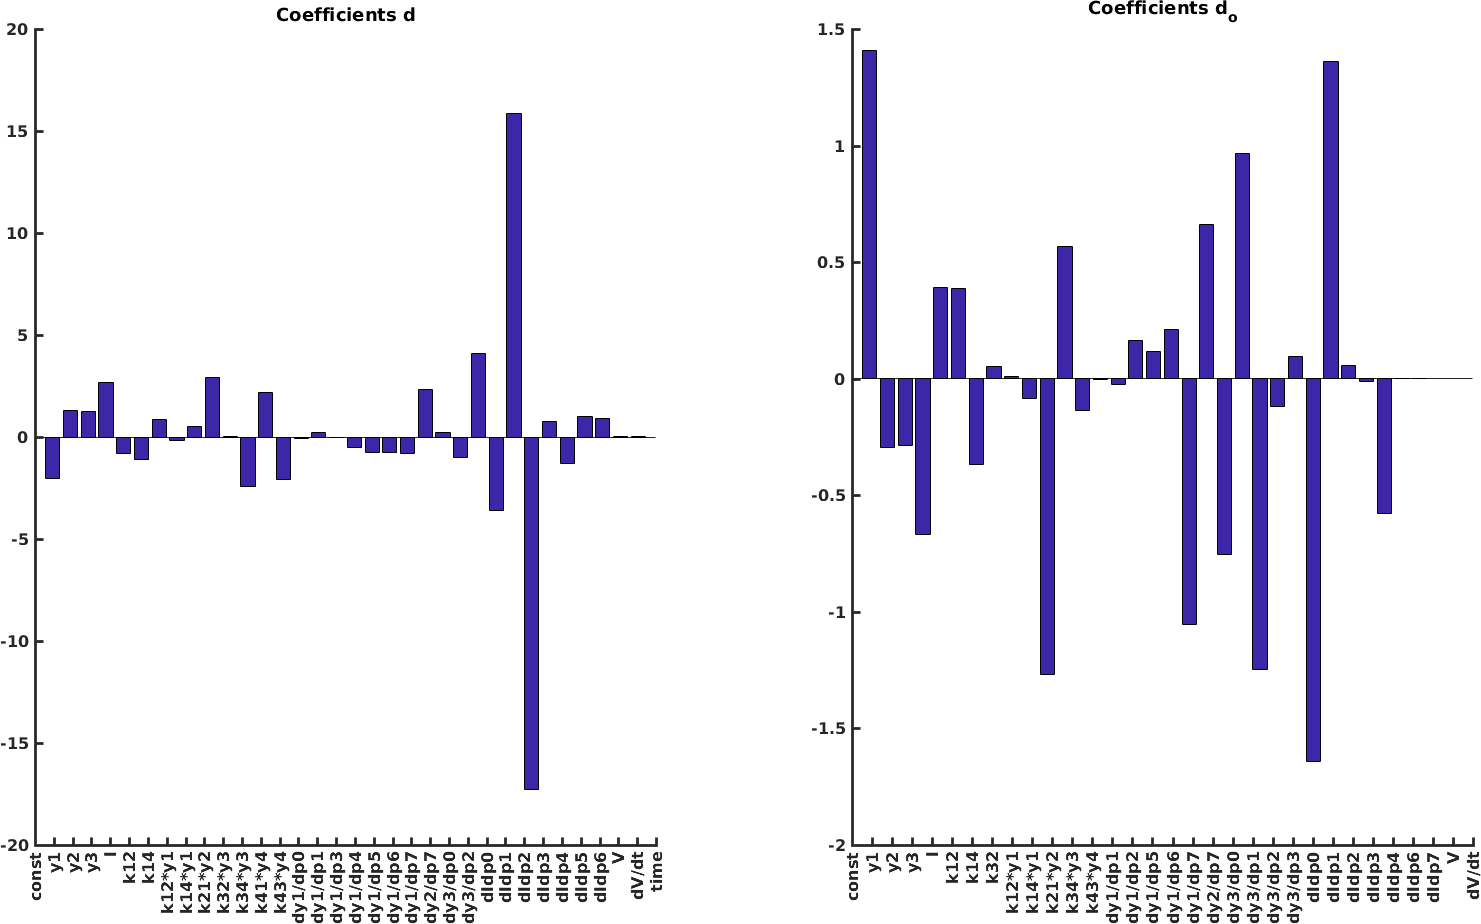
\includegraphics[scale=0.42]{Figures/LASSO_MWDD_AP_full_coefficients.png}
\caption{\textbf{Coefficients in the linear model of discrepancy constructed using LASSO from the sine wave generated component of the MWDD protocol.} This plot shows the included parameters and coefficients for the model produced by LASSO shown in Fig.~\ref{Fig_LASSO_MWDD_AP_full_discrepancy} and Fig.~\ref{Fig_LASSO_MWDD_AP_full_currents}. Coefficients for $d$ are shown on the left, and coefficients for $d_o$ are shown on the right.} 
\label{Fig_LASSO_MWDD_AP_full_coefficients}
\end{center}
\end{figure}

\begin{figure}[hb]
\begin{center}
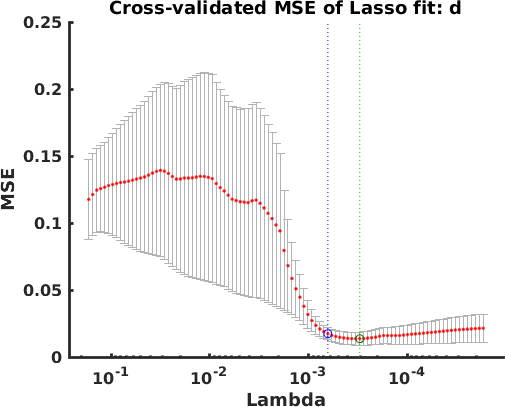
\includegraphics[scale=0.42]{Figures/LASSO_MWDD_AP_full_lambda_d.png}
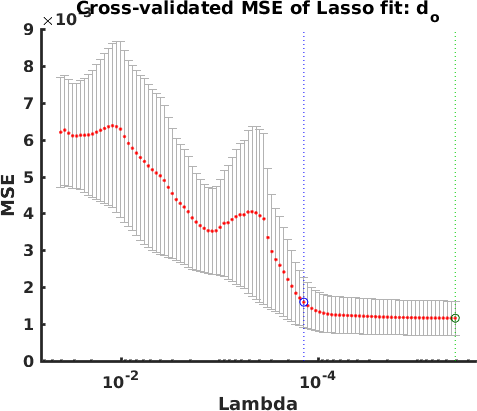
\includegraphics[scale=0.42]{Figures/LASSO_MWDD_AP_full_lambda_od.png}
\caption{\textbf{$\lambda$ and Mean Squared Error plots from the linear models of the sine wave component of the MWDD protocol.} The models of $d$ (left) and $d_o$ (right) have been generated by varying $\lambda$. The error bars indicate the standard error in the MSE between folds. The value of $\lambda$ giving the minimum MSE is indicated by the green line and the selected value of $\lambda$, being the largest value of $\lambda$ with an MSE within one standard error of the minimum, is shown in blue. Note that $\lambda$ runs from largest to smallest, so that the largest model is on the left.}
\label{Fig_LASSO_MWDD_AP_full_lambda}
\end{center}
\end{figure}

\clearpage

\begin{figure}[t]
\begin{center}
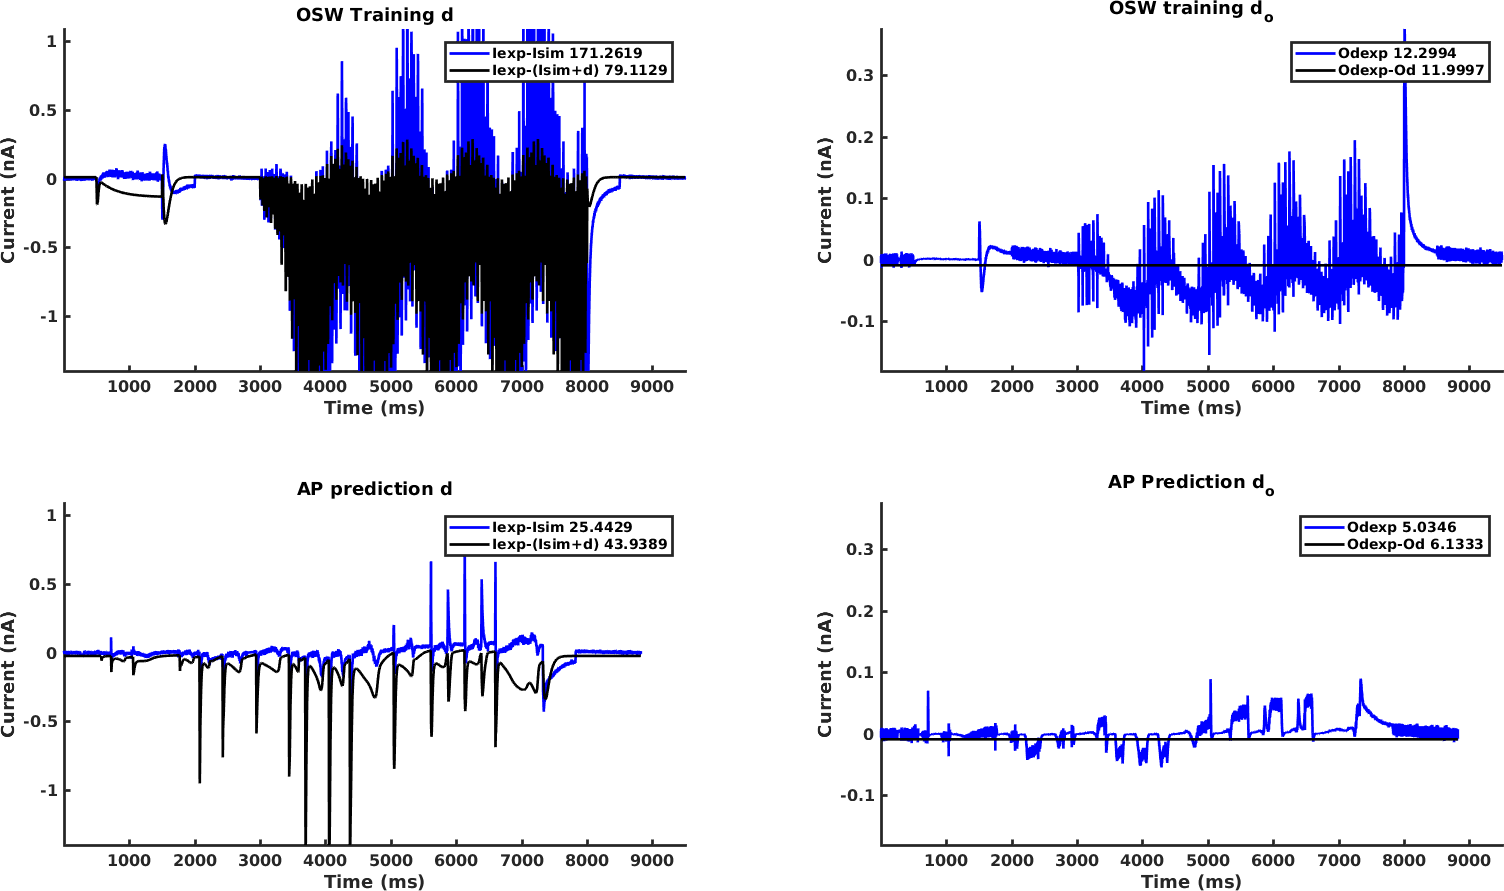
\includegraphics[scale=0.42]{Figures/LASSO_OSW_AP_full_discrepancy.png}
\caption{\textbf{Linear model of discrepancy constructed using LASSO from the OSW protocol.} These models of $d$ (left) and $d_o$ (right) were constructed using LASSO on the entire OSW trace (top), starting with all linearly independent predictors. The root mean square errors between the simulated and predicted traces are shown in the legends. } 
\label{Fig_LASSO_OSW_AP_full_discrepancy}
\end{center}
\end{figure}

\begin{figure}[hb]
\begin{center}
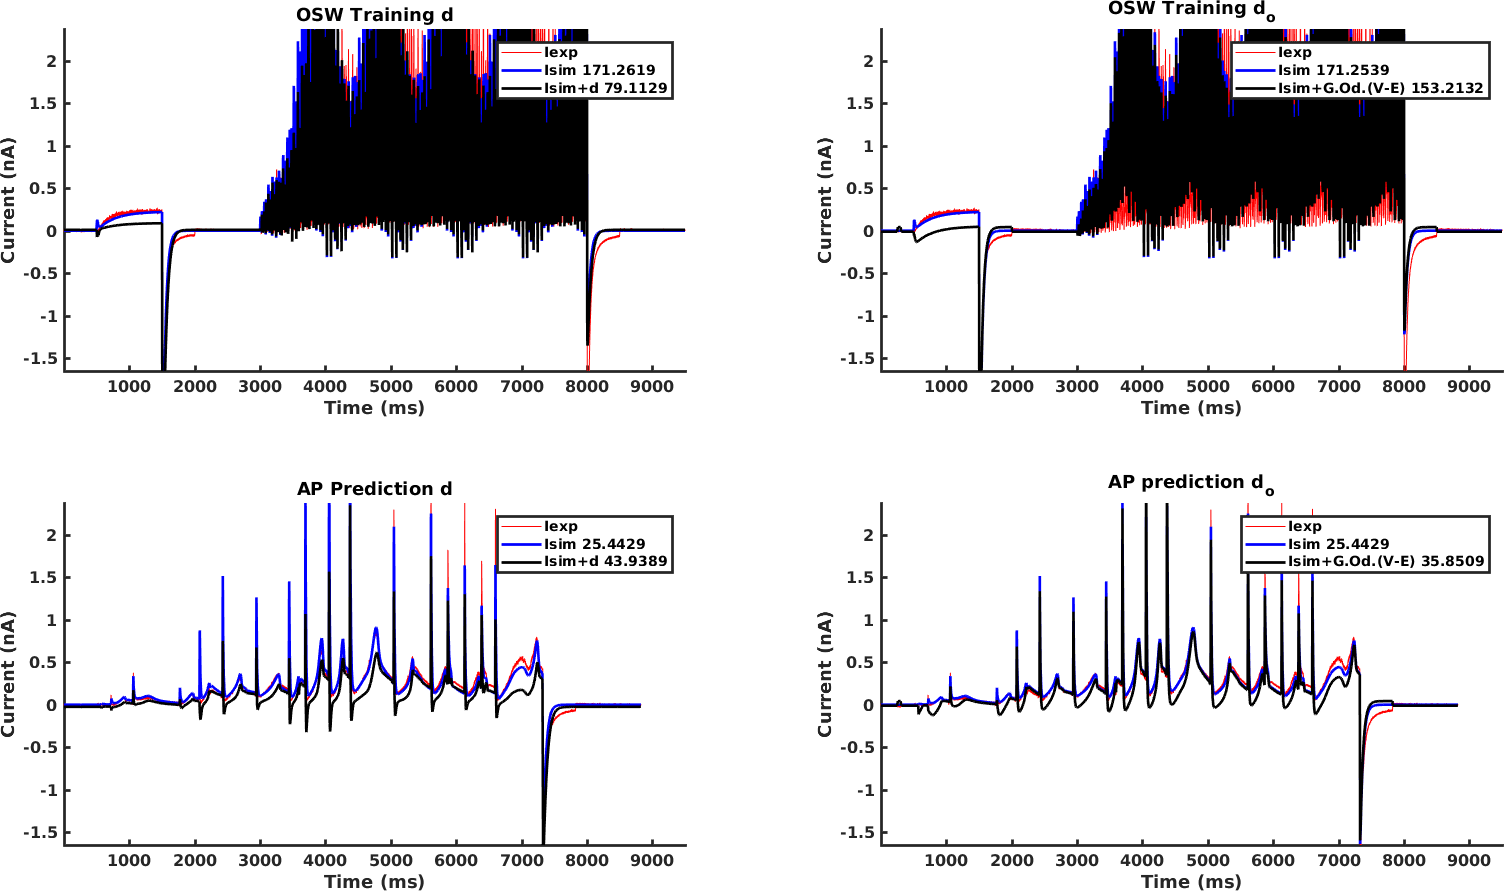
\includegraphics[scale=0.42]{Figures/LASSO_OSW_AP_full_currents.png}
\caption{\textbf{Corrected currents using a linear model of discrepancy constructed using LASSO from the OSW protocol.} The models of $d$ (left) and $d_o$ (right) in Fig. ~\ref{Fig_LASSO_OSW_AP_full_discrepancy} have been incorporated into the simulation (blue line), giving a revised prediction for the OSW and AP protocols (black line). The sum of squared errors between the models and the data are shown in the legend.}
\label{Fig_LASSO_OSW_AP_full_currents}
\end{center}
\end{figure}

\clearpage

\begin{figure}[t]
\begin{center}
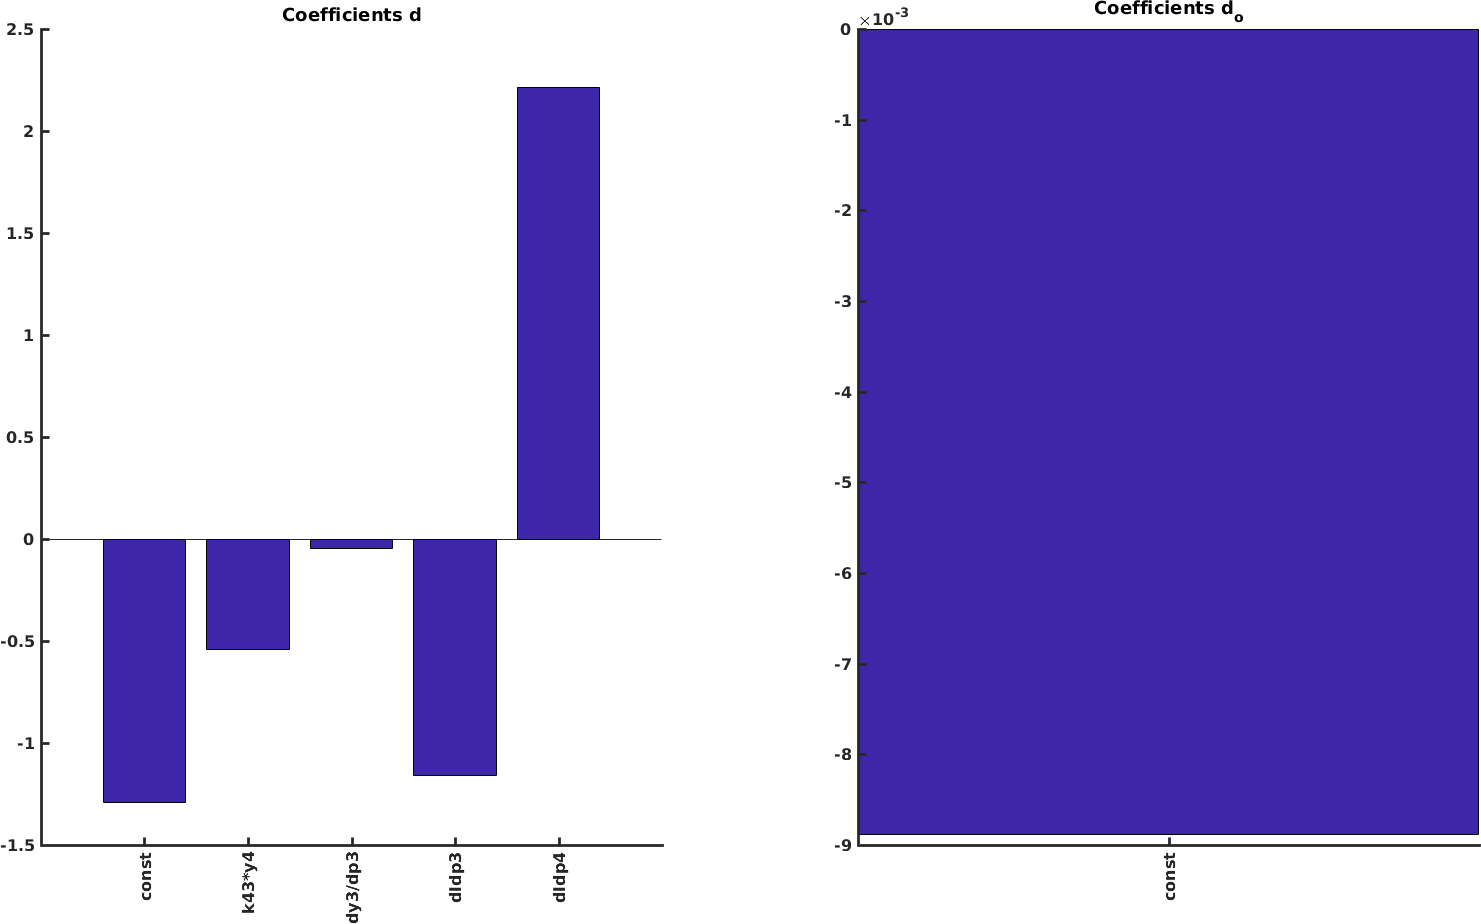
\includegraphics[scale=0.42]{Figures/LASSO_OSW_AP_full_coefficients.png}
\caption{\textbf{Coefficients in the linear model of discrepancy constructed using LASSO from the sine wave generated component of the OSW protocol.} This plot shows the included parameters and coefficients for the model produced by LASSO shown in Fig.~\ref{Fig_LASSO_OSW_AP_full_discrepancy} and Fig.~\ref{Fig_LASSO_OSW_AP_full_currents}. Coefficients for $d$ are shown on the left, and coefficients for $d_o$ are shown on the right.} 
\label{Fig_LASSO_OSW_AP_full_coefficients}
\end{center}
\end{figure}

\begin{figure}[hb]
\begin{center}
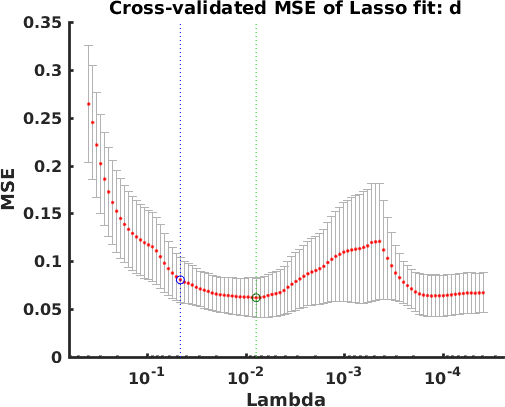
\includegraphics[scale=0.42]{Figures/LASSO_OSW_AP_full_lambda_d.png}
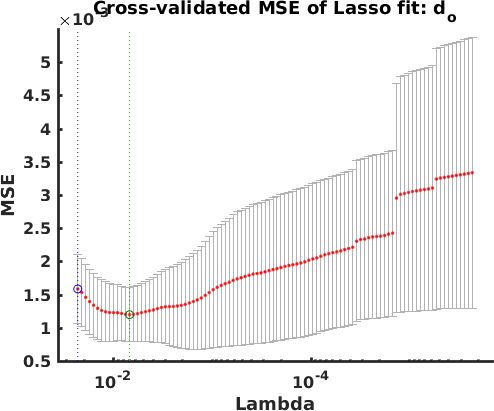
\includegraphics[scale=0.42]{Figures/LASSO_OSW_AP_full_lambda_od.png}
\caption{\textbf{$\lambda$ and Mean Squared Error plots from the linear models of the sine wave component of the OSW protocol.} The models of $d$ (left) and $d_o$ (right) have been generated by varying $\lambda$. The error bars indicate the standard error in the MSE between folds. The value of $\lambda$ giving the minimum MSE is indicated by the green line and the selected value of $\lambda$, being the largest value of $\lambda$ with an MSE within one standard error of the minimum, is shown in blue. Note that $\lambda$ runs from largest to smallest, so that the largest model is on the left.}
\label{Fig_LASSO_OSW_AP_core_lambda}
\end{center}
\end{figure}

\clearpage

\begin{figure}[t]
\begin{center}
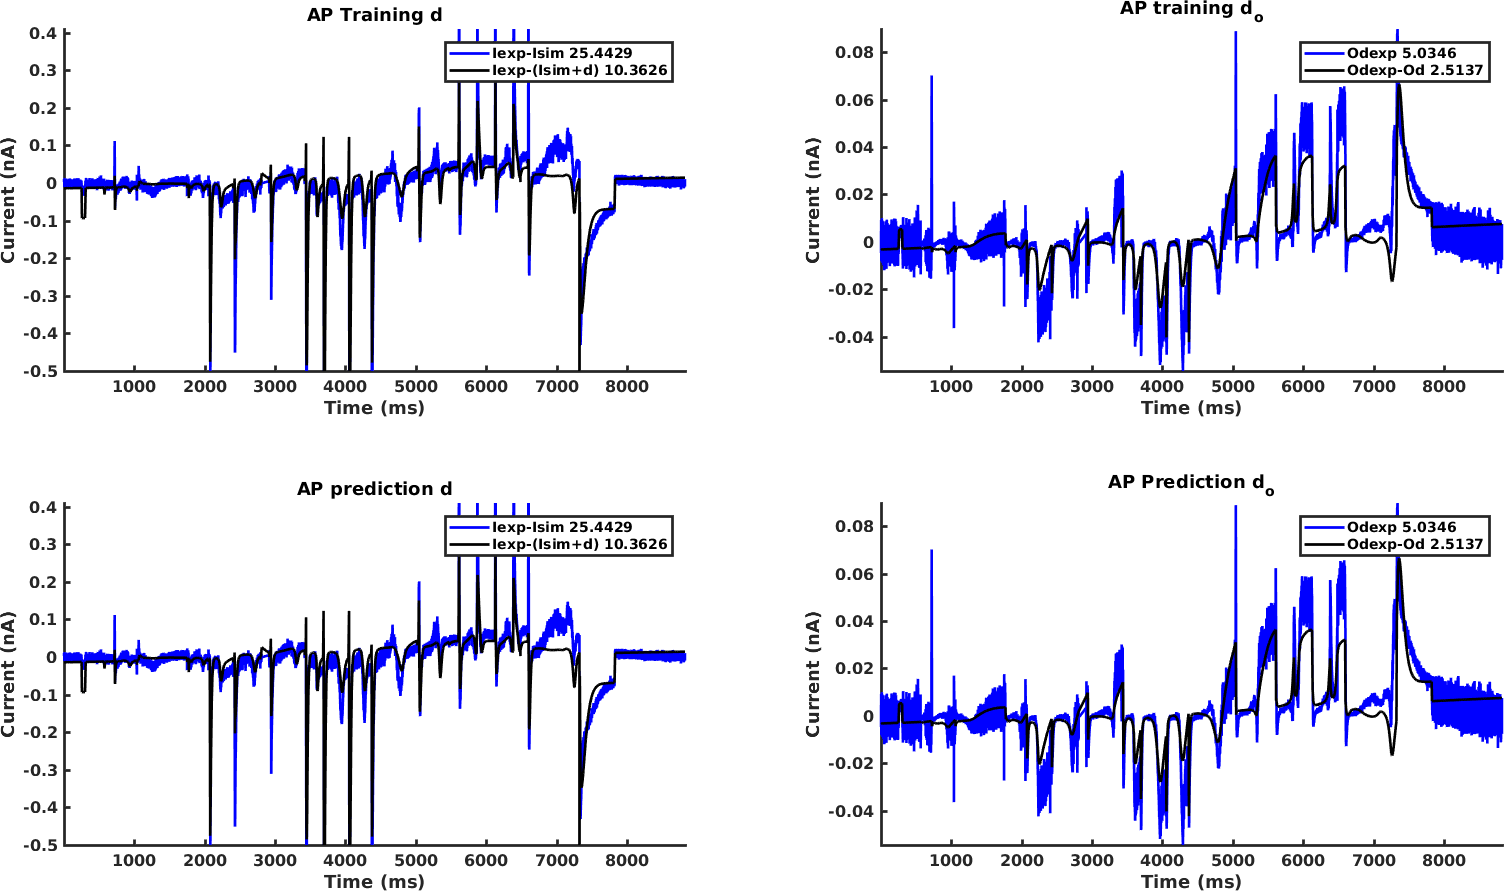
\includegraphics[scale=0.42]{Figures/LASSO_AP_AP_full_discrepancy.png}
\caption{\textbf{Linear model of discrepancy constructed using LASSO from the AP protocol.} These models of $d$ (left) and $d_o$ (right) were constructed using LASSO on the entire AP trace (top), starting with all linearly independent predictors. The root mean square errors between the simulated and predicted traces are shown in the legends. } 
\label{Fig_LASSO_AP_AP_full_discrepancy}
\end{center}
\end{figure}

\begin{figure}[hb]
\begin{center}
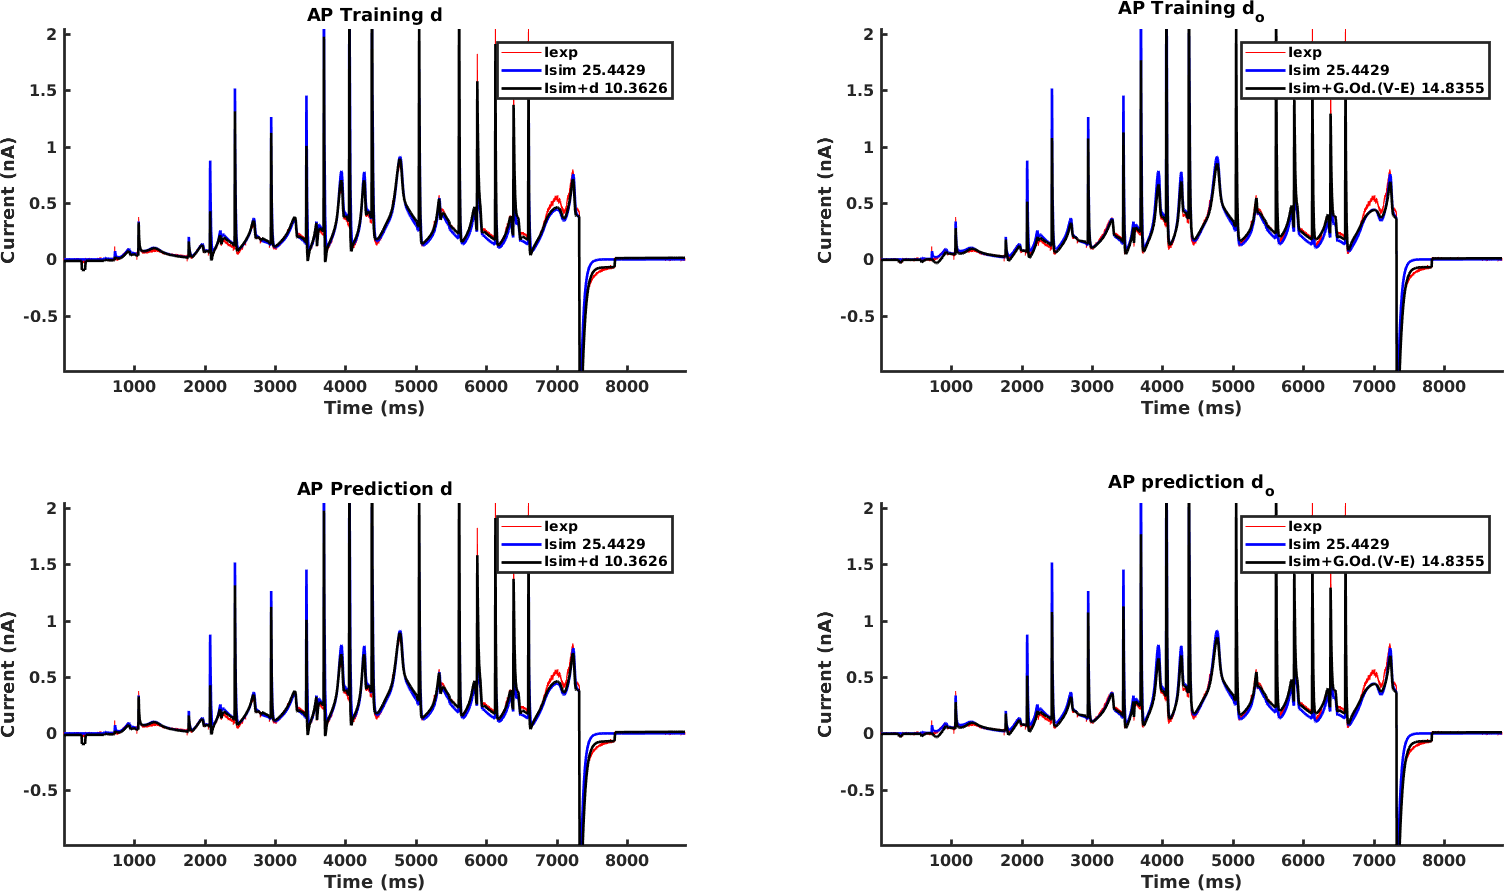
\includegraphics[scale=0.42]{Figures/LASSO_AP_AP_full_currents.png}
\caption{\textbf{Corrected currents using a linear model of discrepancy constructed using LASSO from the AP protocol.} The models of $d$ (left) and $d_o$ (right) in Fig. ~\ref{Fig_LASSO_AP_AP_full_discrepancy} have been incorporated into the simulation (blue line), giving a revised prediction for the AP protocol (black line). The sum of squared errors between the models and the data are shown in the legend.}
\label{Fig_LASSO_AP_AP_full_currents}
\end{center}
\end{figure}

\clearpage

\begin{figure}[t]
\begin{center}
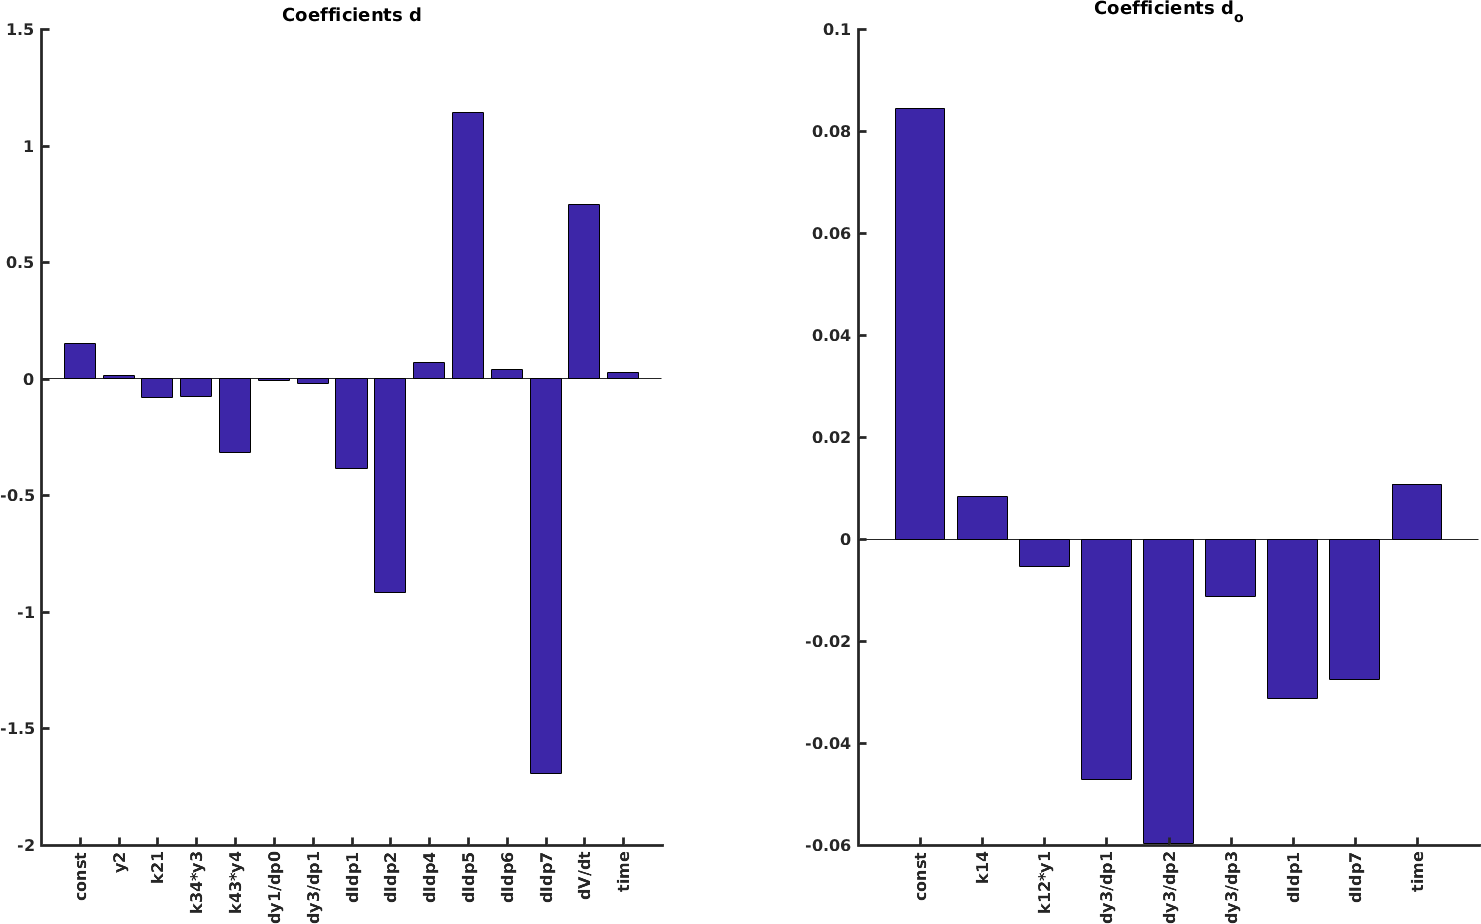
\includegraphics[scale=0.42]{Figures/LASSO_AP_AP_full_coefficients.png}
\caption{\textbf{Coefficients in the linear model of discrepancy constructed using LASSO from the sine wave generated component of the AP protocol.} This plot shows the included parameters and coefficients for the model produced by LASSO shown in Fig.~\ref{Fig_LASSO_AP_AP_full_discrepancy} and Fig.~\ref{Fig_LASSO_AP_AP_full_currents}. Coefficients for $d$ are shown on the left, and coefficients for $d_o$ are shown on the right.} 
\label{Fig_LASSO_AP_AP_full_coefficients}
\end{center}
\end{figure}

\begin{figure}[hb]
\begin{center}
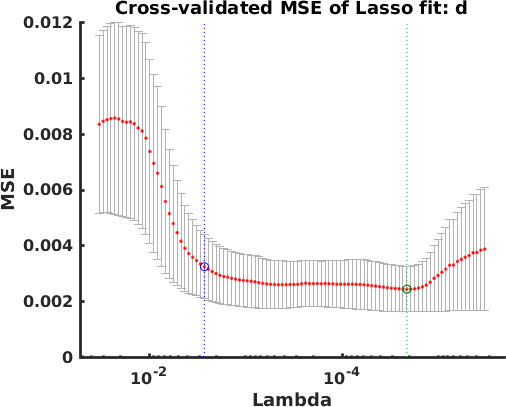
\includegraphics[scale=0.42]{Figures/LASSO_AP_AP_full_lambda_d.png}
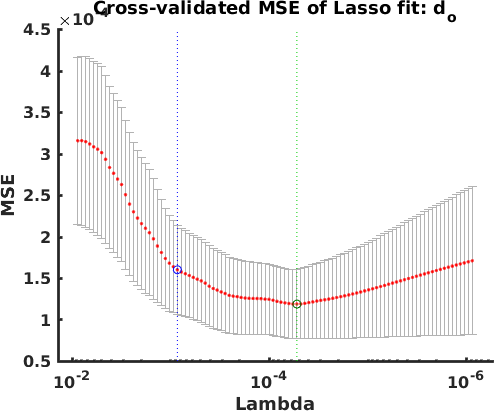
\includegraphics[scale=0.42]{Figures/LASSO_AP_AP_full_lambda_od.png}
\caption{\textbf{$\lambda$ and Mean Squared Error plots from the linear models of the sine wave component of the AP protocol.} The models of $d$ (left) and $d_o$ (right) have been generated by varying $\lambda$. The error bars indicate the standard error in the MSE between folds. The value of $\lambda$ giving the minimum MSE is indicated by the green line and the selected value of $\lambda$, being the largest value of $\lambda$ with an MSE within one standard error of the minimum, is shown in blue. Note that $\lambda$ runs from largest to smallest, so that the largest model is on the left.}
\label{Fig_LASSO_AP_AP_full_lambda}
\end{center}
\end{figure}

\clearpage

\subsection{Predicting Discrepancy Using Stepwise Linear Model}\label{SubSec_StepwiseLM_Discrepancy}
\subsubsection{The Method}
Stepwise Linear Model (StepwiseLM) is a Matlab method for constructing linear models using a stepwise approach\footnote{\url{https://www.mathworks.com/help/stats/stepwiselm.html}}. The method includes predictors in a stepwise manner by first building  up a model by examining all non-included predictors, checking if any have a value below a set entrance tolerance, then including the predictor with the smallest value in the model. Once no more terms can be added to the model, the reverse process is applied and terms are removed from the model if they exceed a removal value. Further terms are then added as before. The final model is then produced when no more predictors can be removed from the model. The method also allows for higher order terms such as interactions and quadratic terms. Initial experiments showed that this approach led to high degrees of overfitting and so was rejected. A number of criteria are available for setting the threshold for including predictors into the model\cite{Wasserman2010}, being
\begin{itemize}
\item $F$-test of the change in the sum of squared error 
\item Aikake Information Criterion (AIC), $\mathcal{l}S-|S|$ where $\mathcal{l}S$ is the log-likelihood of the model $S$ evaluated at the maximum likelihood estimate, and $|S|$ is the number of predictors in the model.
\item Bayesian Information Criterion (BIC), $\mathcal{l}S-\frac{|S|}{2} \log( n )$, where $n$ is the number of data points. BIC penalizes model size more heavily than AIC.
\item Increase in $R^2$
\item Increase in adjusted $R^2$
\end{itemize}
For the plots in Section \ref{SubSubSec_StepwiseLM_Results}, we used AIC with the Matlab default values for entering ($0$) and removal from ($0.1$) the model. 

The StepwiseLM method has the appealing feature that it can include polynomial interaction terms to arbitrary order, for example interactions ($X_iX_j$) or quadratic terms ($X_i^2$). Preliminary experiments found that these methods resulted in an enormous degree of overfitting and very poor prediction. Consequently, they have been omitted from this report.

\subsubsection{Results}\label{SubSubSec_StepwiseLM_Results}
This section shows the same data as for the LASSO results shown above in Section \ref{SubSec_Lasso_Discrepancy}. Because stepwiselm does not use regularization, no lambda plots are shown. In general, the model tended to overfit, rather than underfit as for LASSO. As a result, the general trend is for a reasonable fit to the training data but a poor fit during prediction.

\begin{figure}[t]
\begin{center}
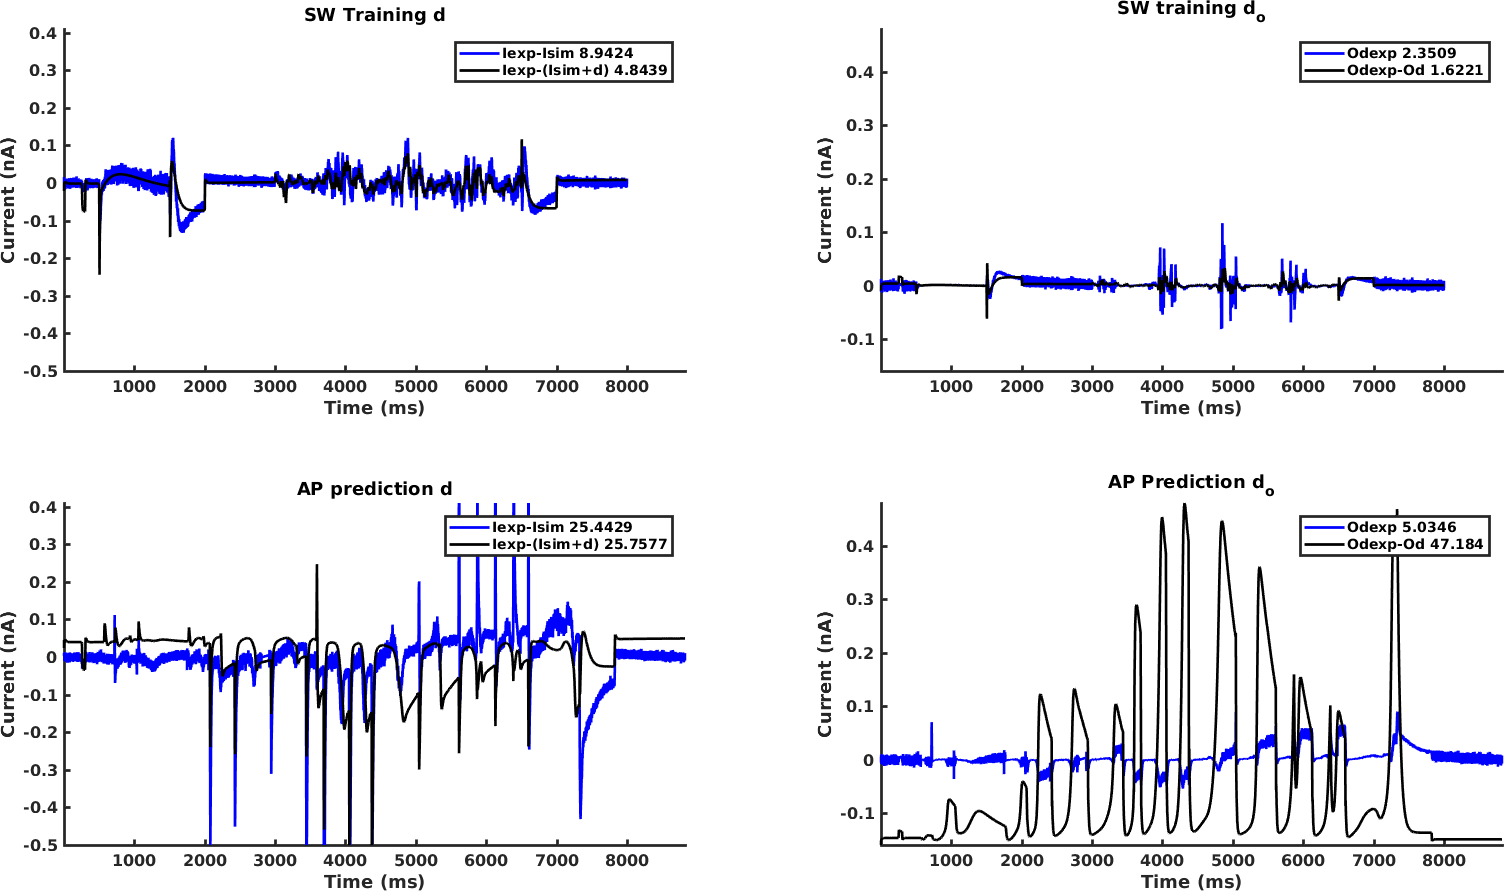
\includegraphics[scale=0.42]{Figures/StepwiseLM_SW_AP_full_discrepancy.png}
\caption{\textbf{Linear model of discrepancy constructed using StepwiseLM from the SW protocol.} These models of $d$ (left) and $d_o$ (right) were constructed using StepwiseLM on the entire SW trace (top), starting with all linearly independent predictors. The improvement of the training trace (top) is poor and the resulting models fail to predict the discrepancy in the AP trace (bottom). The root mean square errors between the simulated and predicted traces are shown in the legends. } 
\label{Fig_StepwiseLM_SW_AP_full_discrepancy}
\end{center}
\end{figure}

\begin{figure}[hb]
\begin{center}
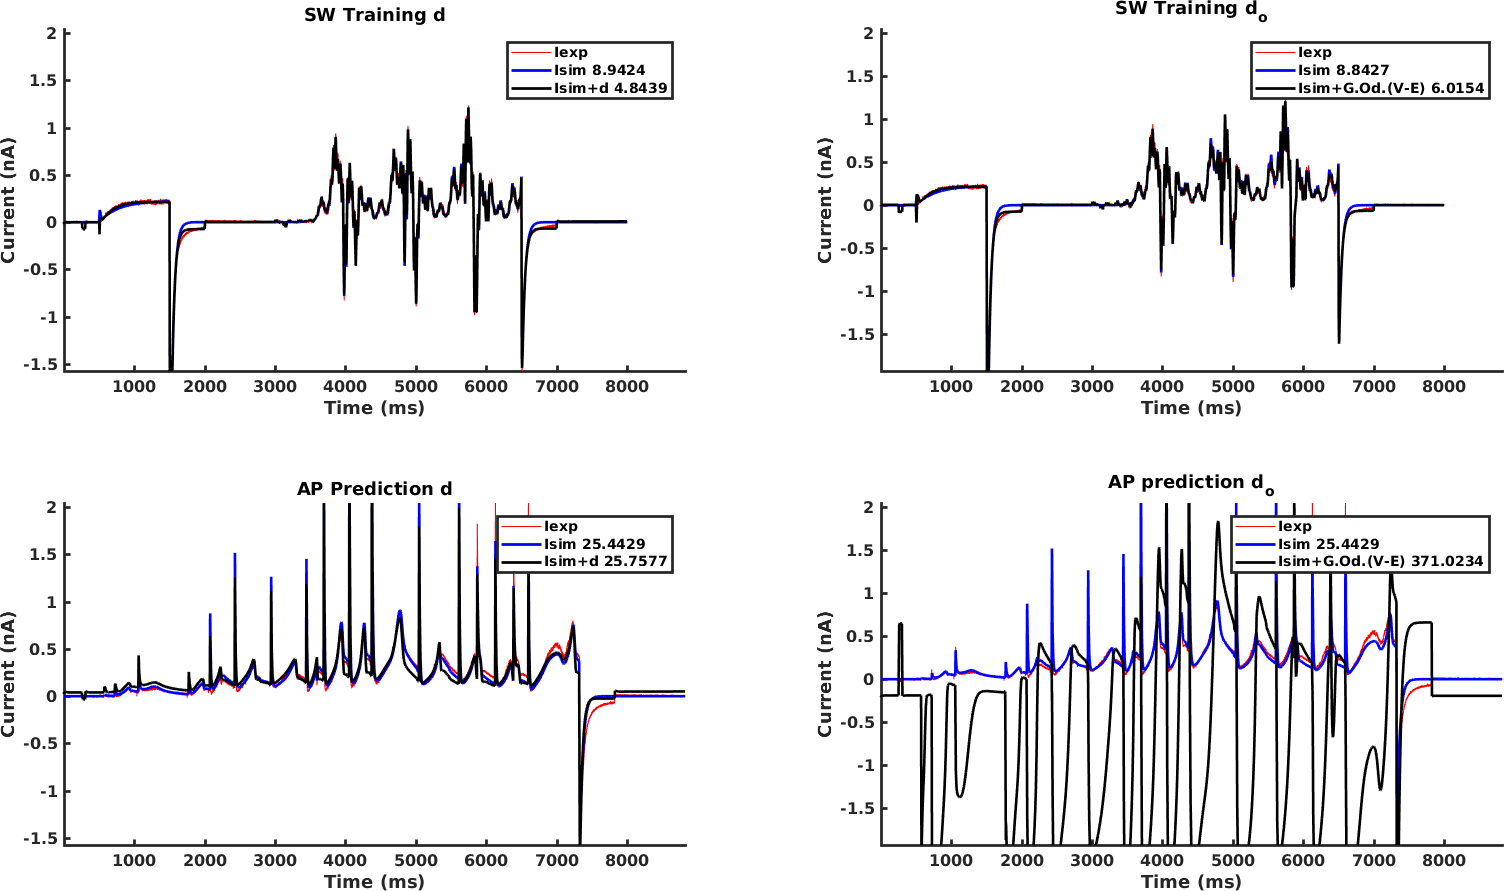
\includegraphics[scale=0.42]{Figures/StepwiseLM_SW_AP_full_currents.png}
\caption{\textbf{Corrected currents using a linear model of discrepancy constructed using StepwiseLM from the SW protocol.} The models of $d$ (left) and $d_o$ (right) in Fig. ~\ref{Fig_StepwiseLM_SW_AP_full_discrepancy} have been incorporated into the simulation (blue line), giving a revised prediction for the SW and AP protocols (black line). As expected from Fig.~\ref{Fig_StepwiseLM_SW_AP_full_discrepancy}, there is little improvement in the agreement with the experimental data (red line). The sum of squared errors between the models and the data are shown in the legend.}
\label{Fig_StepwiseLM_SW_AP_full_currents}
\end{center}
\end{figure}

\begin{figure}[t]
\begin{center}
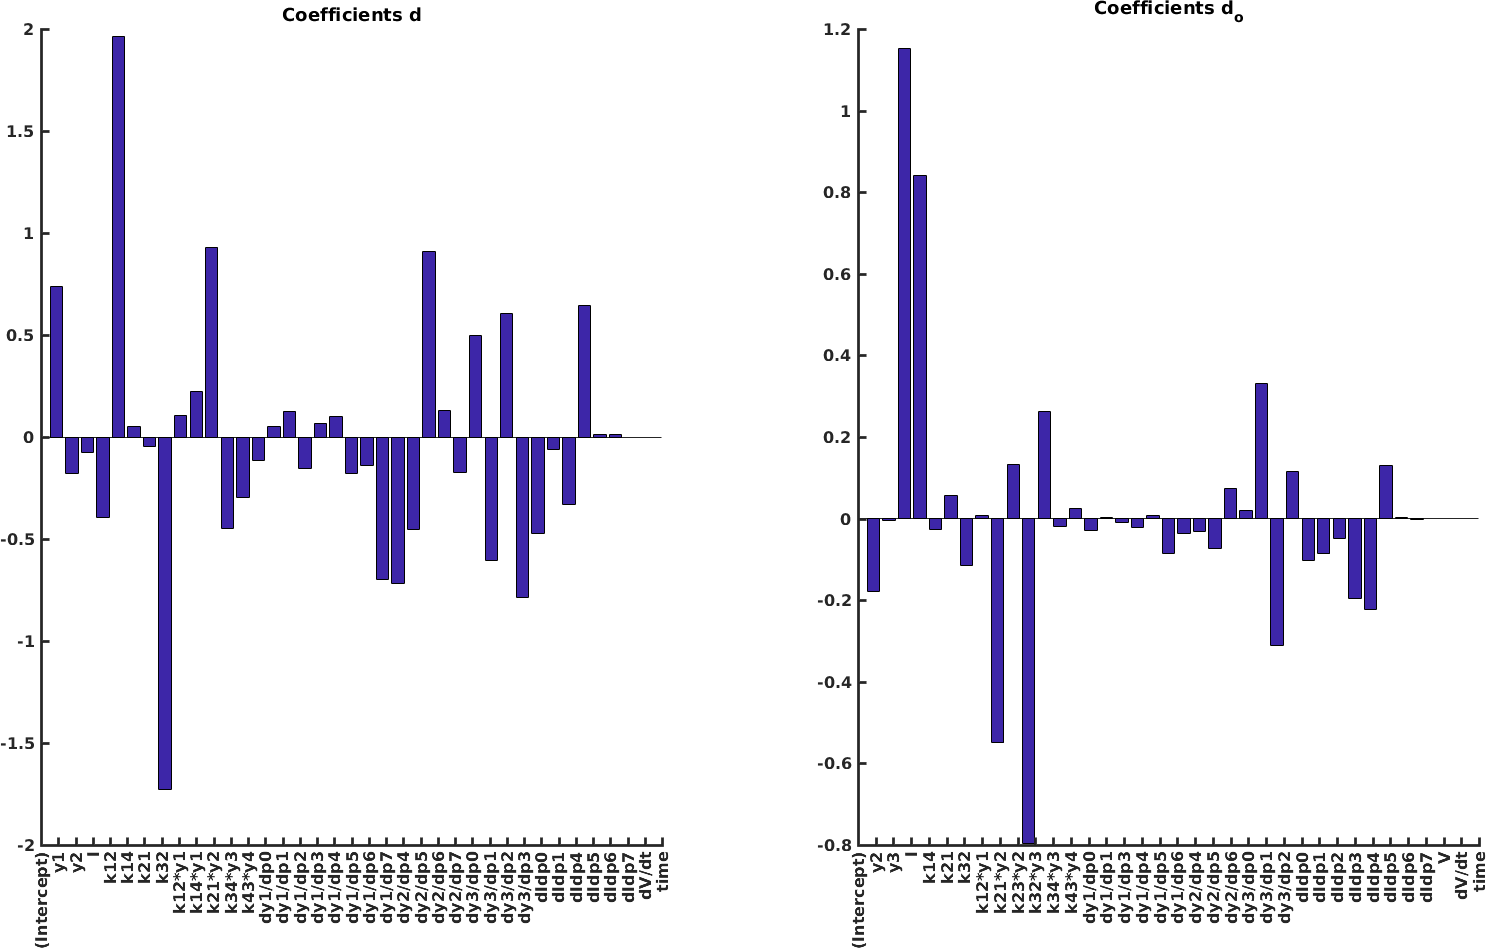
\includegraphics[scale=0.42]{Figures/StepwiseLM_SW_AP_full_coefficients.png}
\caption{\textbf{Coefficients in the linear model of discrepancy constructed using StepwiseLM from the SW protocol.} This plot shows the included parameters and coefficients for the model produced by StepwiseLM shown in Fig.~\ref{Fig_StepwiseLM_SW_AP_full_discrepancy} and Fig.~\ref{Fig_StepwiseLM_SW_AP_full_currents}. Coefficients for $d$ are shown on the left, and coefficients for $d_o$ are shown on the right.} 
\label{Fig_StepwiseLM_SW_AP_coefficients}
\end{center}
\end{figure}

\clearpage

\begin{figure}[t]
\begin{center}
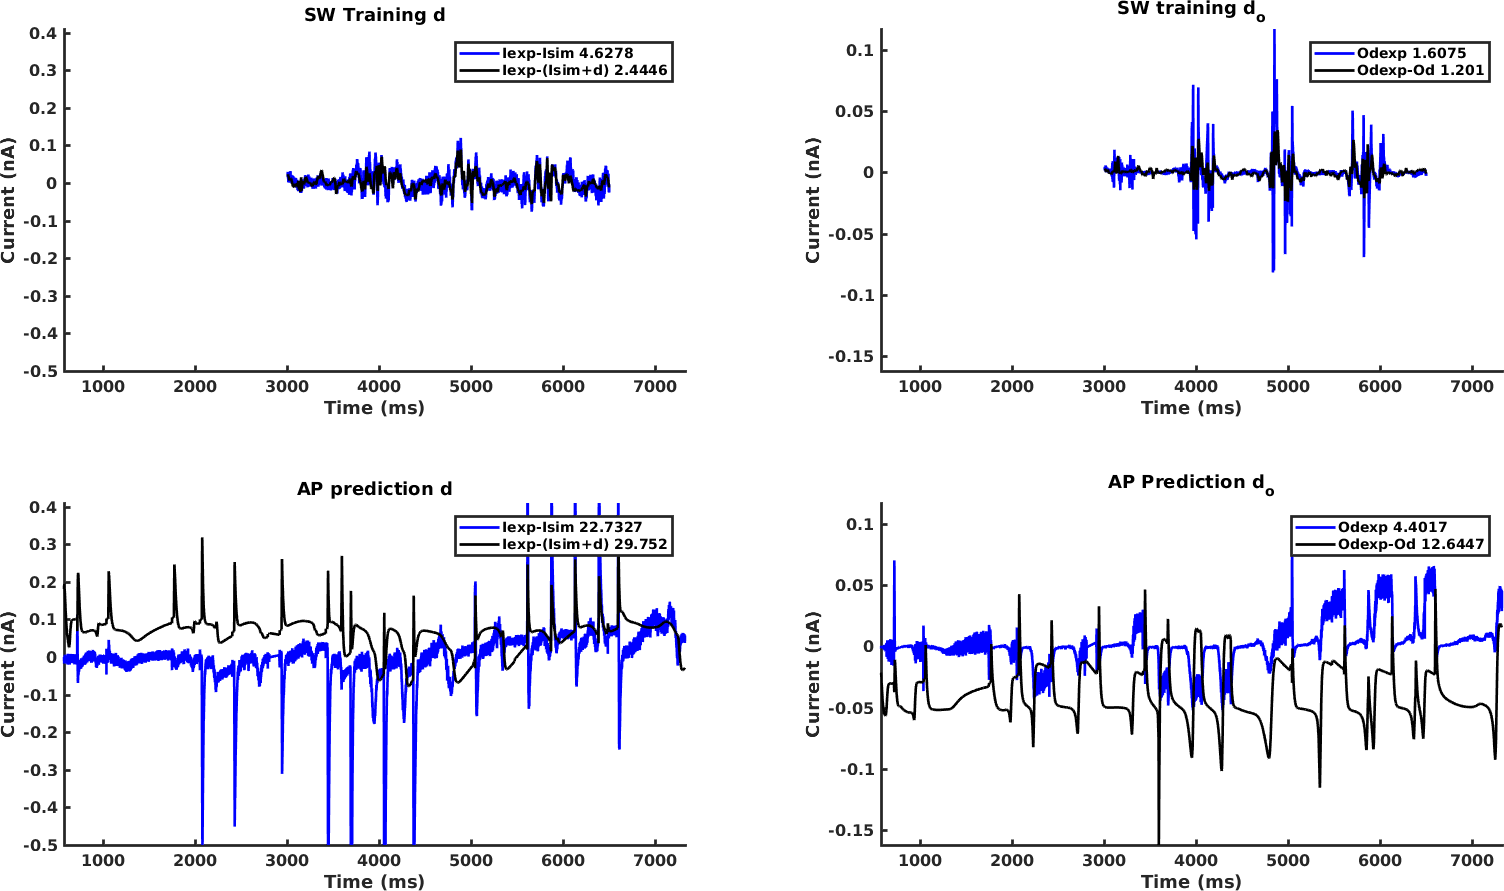
\includegraphics[scale=0.42]{Figures/StepwiseLM_SW_AP_core_discrepancy.png}
\caption{\textbf{Linear model of discrepancy constructed using StepwiseLM.} These models of $d$ (left) and $d_o$ (right) were constructed using StepwiseLM on the entire SW trace (top), starting with all linearly independent predictors. The root mean square errors between the simulated and predicted traces are shown in the legends. } 
\label{Fig_StepwiseLM_SW_AP_core_discrepancy}
\end{center}
\end{figure}

\begin{figure}[hb]
\begin{center}
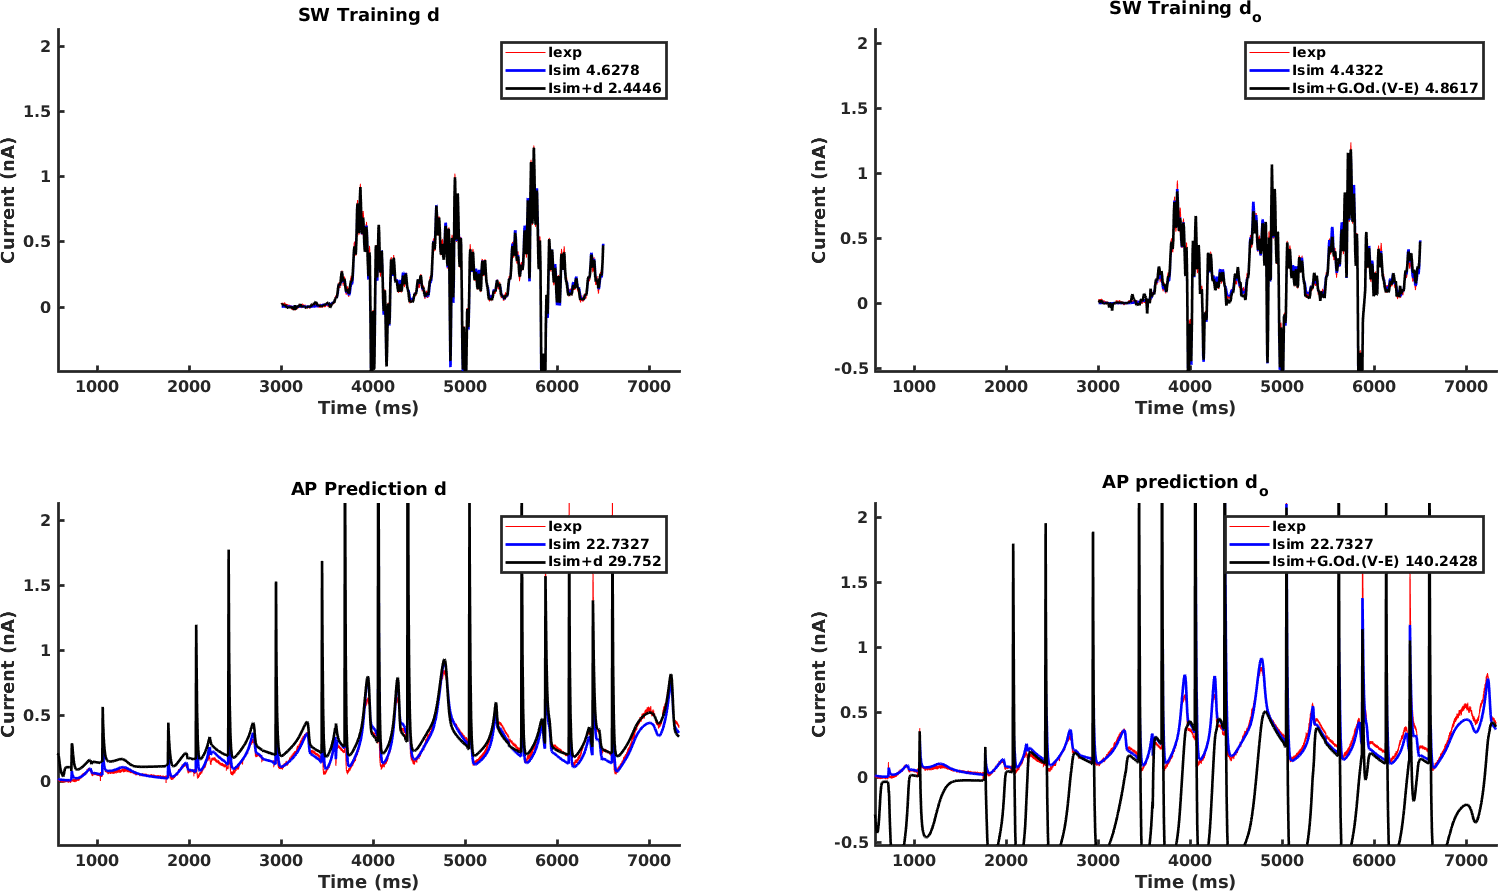
\includegraphics[scale=0.42]{Figures/StepwiseLM_SW_AP_core_currents.png}
\caption{\textbf{Corrected currents using a linear model of discrepancy constructed using StepwiseLM from the sine wave generated component of the SW protocol.} The models of $d$ (left) and $d_o$ (right) in Fig.~\ref{Fig_StepwiseLM_SW_AP_core_discrepancy} have been incorporated into the simulation (blue line), giving a revised prediction for the SW and AP protocols (black line). The sum of squared errors between the models and the data are shown in the legend.}
\label{Fig_StepwiseLM_SW_AP_core_currents}
\end{center}
\end{figure}

\clearpage

\begin{figure}[t]
\begin{center}
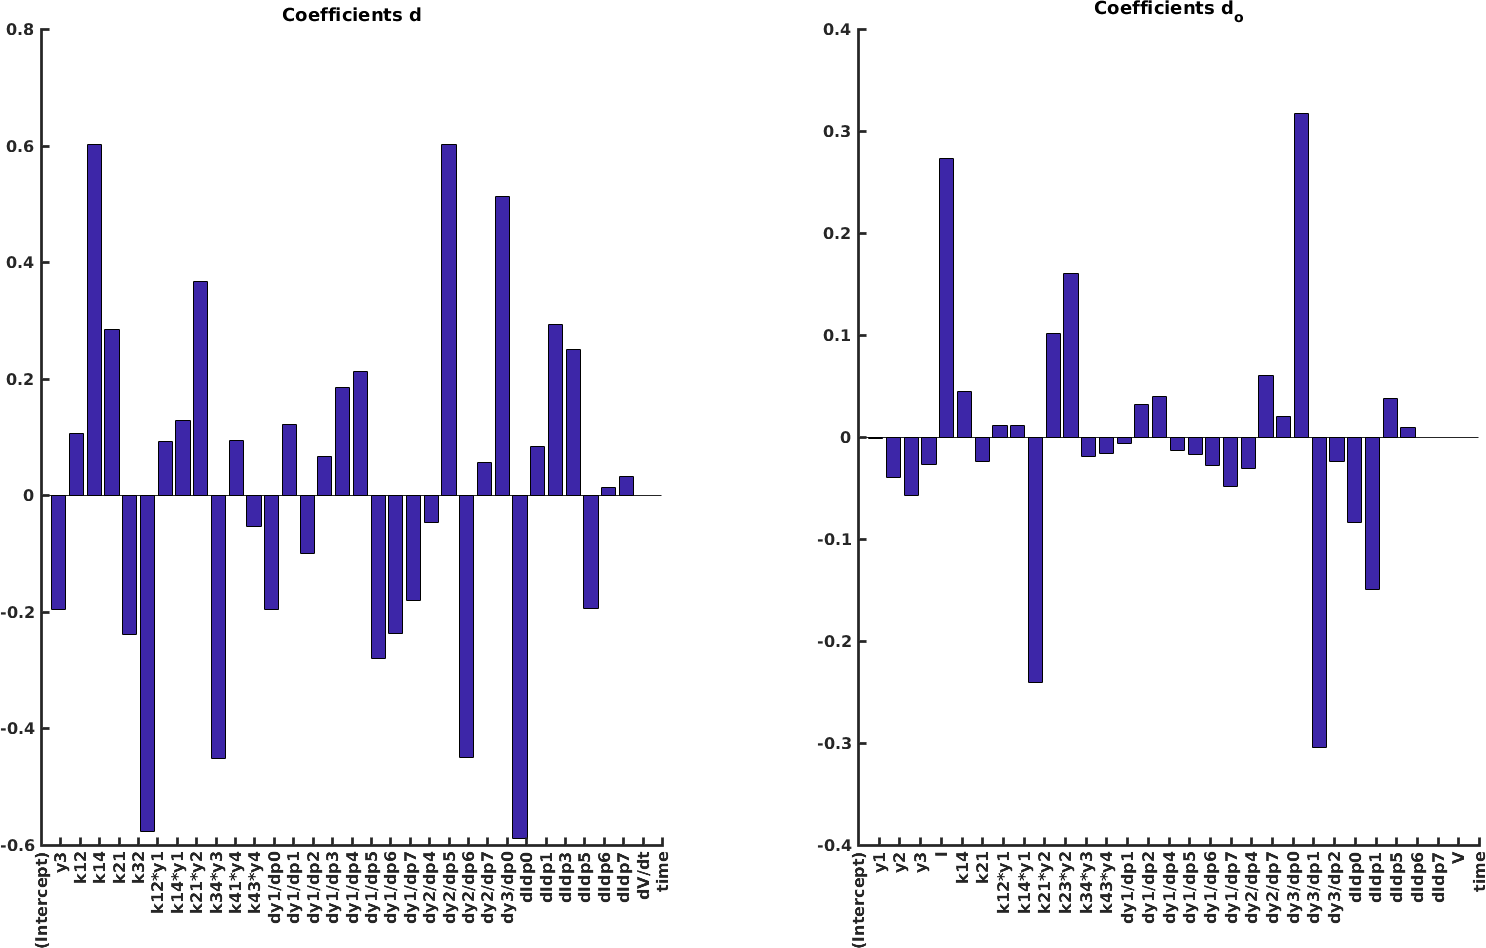
\includegraphics[scale=0.42]{Figures/StepwiseLM_SW_AP_core_coefficients.png}
\caption{\textbf{Coefficients in the linear model of discrepancy constructed using StepwiseLM from the sine wave generated component of the SW protocol.} This plot shows the included parameters and coefficients for the model produced by StepwiseLM shown in Fig.~\ref{Fig_StepwiseLM_SW_AP_core_discrepancy} and Fig.~\ref{Fig_StepwiseLM_SW_AP_core_currents}. Coefficients for $d$ are shown on the left, and coefficients for $d_o$ are shown on the right.} 
\label{Fig_StepwiseLM_SW_AP_core_coefficients}
\end{center}
\end{figure}

\clearpage

\begin{figure}[t]
\begin{center}
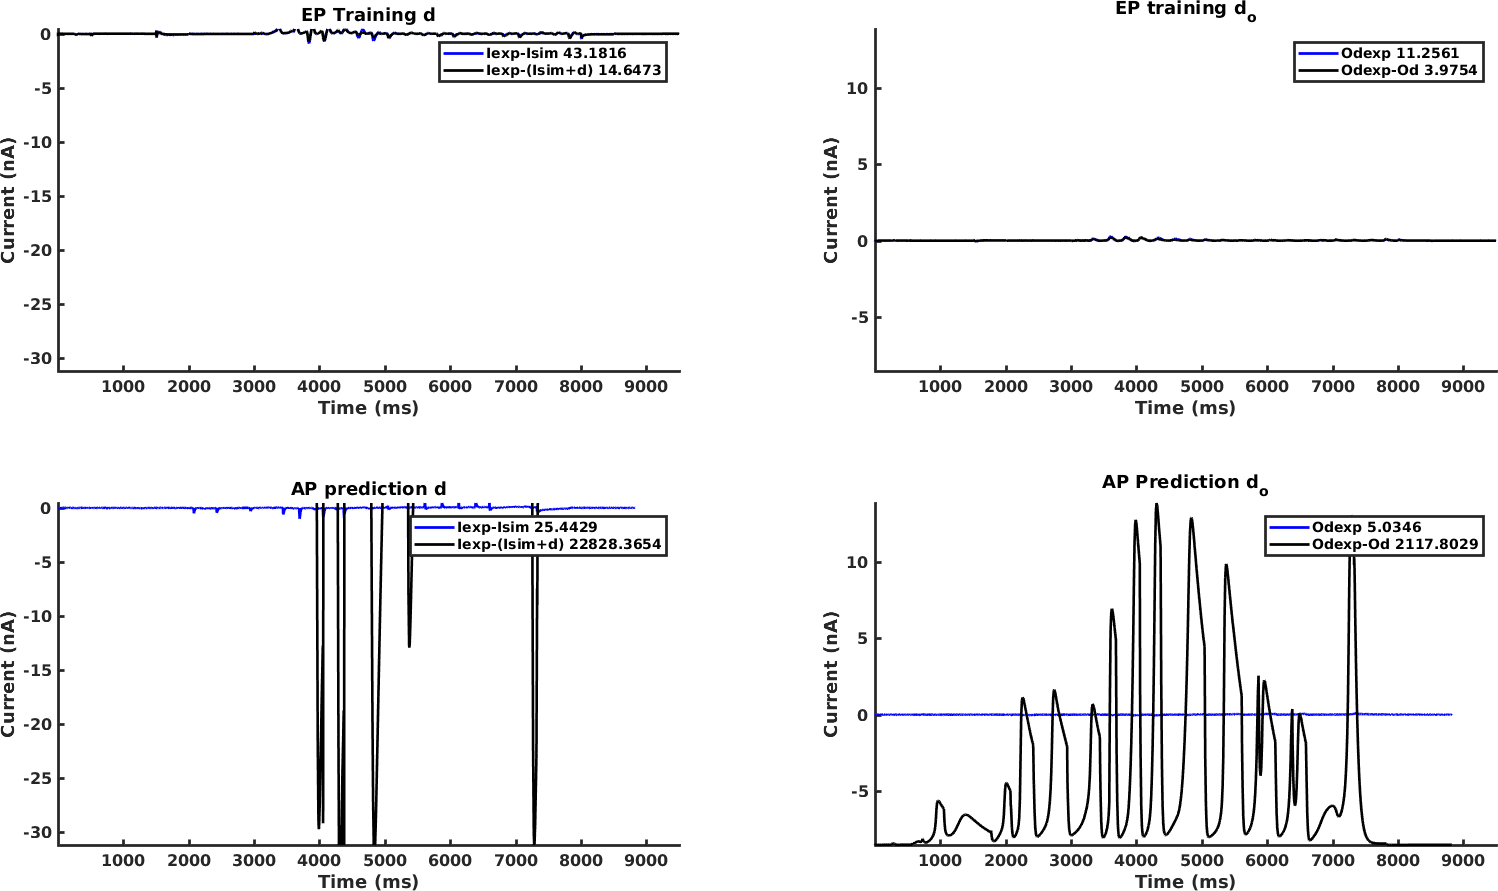
\includegraphics[scale=0.42]{Figures/StepwiseLM_EP_AP_full_discrepancy.png}
\caption{\textbf{Linear model of discrepancy constructed using StepwiseLM from the EP protocol.} These models of $d$ (left) and $d_o$ (right) were constructed using StepwiseLM on the entire SW trace (top), starting with all linearly independent predictors. The root mean square errors between the simulated and predicted traces are shown in the legends. } 
\label{Fig_StepwiseLM_EP_AP_full_discrepancy}
\end{center}
\end{figure}

\begin{figure}[hb]
\begin{center}
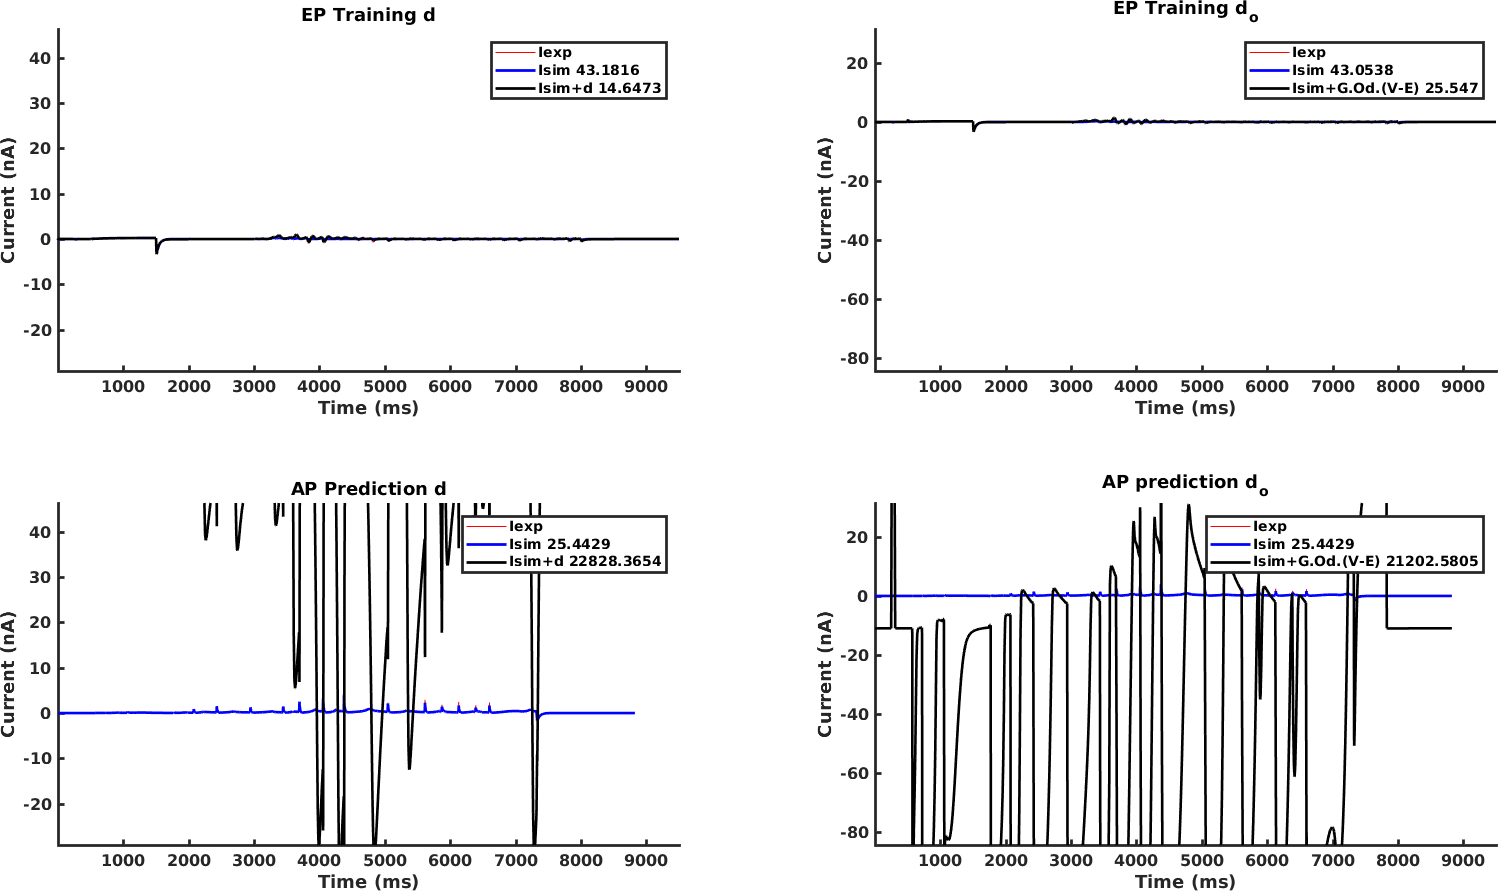
\includegraphics[scale=0.42]{Figures/StepwiseLM_EP_AP_full_currents.png}
\caption{\textbf{Corrected currents using a linear model of discrepancy constructed using StepwiseLM from the EP protocol.} The models of $d$ (left) and $d_o$ (right) in Fig. ~\ref{Fig_StepwiseLM_SW_AP_full_discrepancy} have been incorporated into the simulation (blue line), giving a revised prediction for the EP and AP protocols (black line). The sum of squared errors between the models and the data are shown in the legend.}
\label{Fig_StepwiseLM_EP_AP_full_currents}
\end{center}
\end{figure}

\clearpage

\begin{figure}[t]
\begin{center}
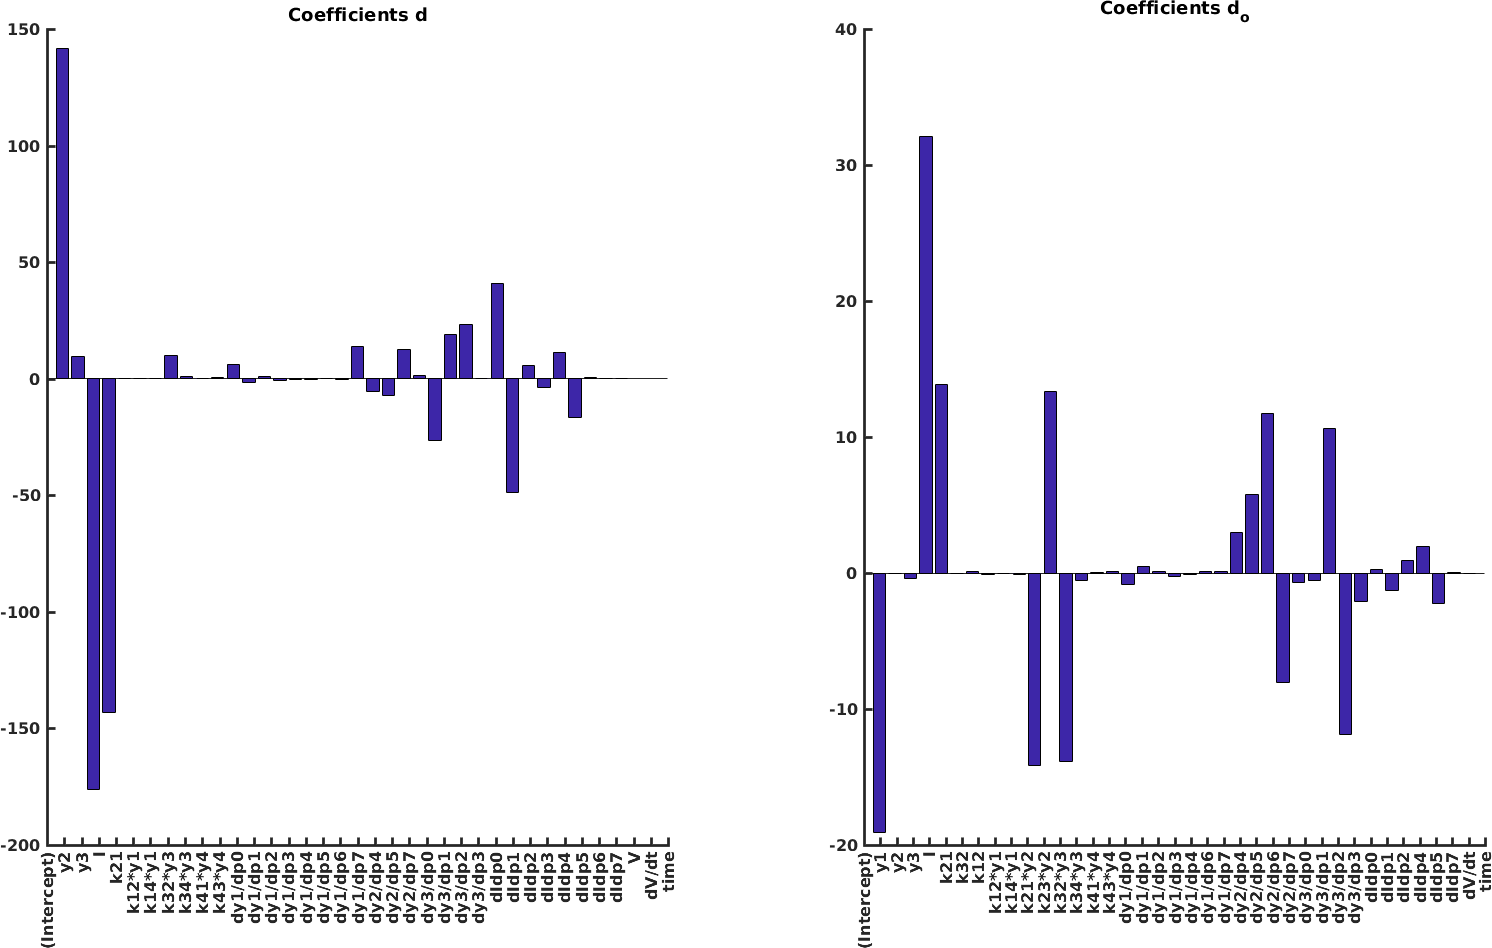
\includegraphics[scale=0.42]{Figures/StepwiseLM_EP_AP_full_coefficients.png}
\caption{\textbf{Coefficients in the linear model of discrepancy constructed using StepwiseLM from the EP protocol.} This plot shows the included parameters and coefficients for the model produced by StepwiseLM shown in Fig.~\ref{Fig_StepwiseLM_EP_AP_full_discrepancy} and Fig.~\ref{Fig_StepwiseLM_EP_AP_full_currents}. Coefficients for $d$ are shown on the left, and coefficients for $d_o$ are shown on the right.} 
\label{Fig_StepwiseLM_EP_AP_full_coefficients}
\end{center}
\end{figure}

\clearpage

\begin{figure}[t]
\begin{center}
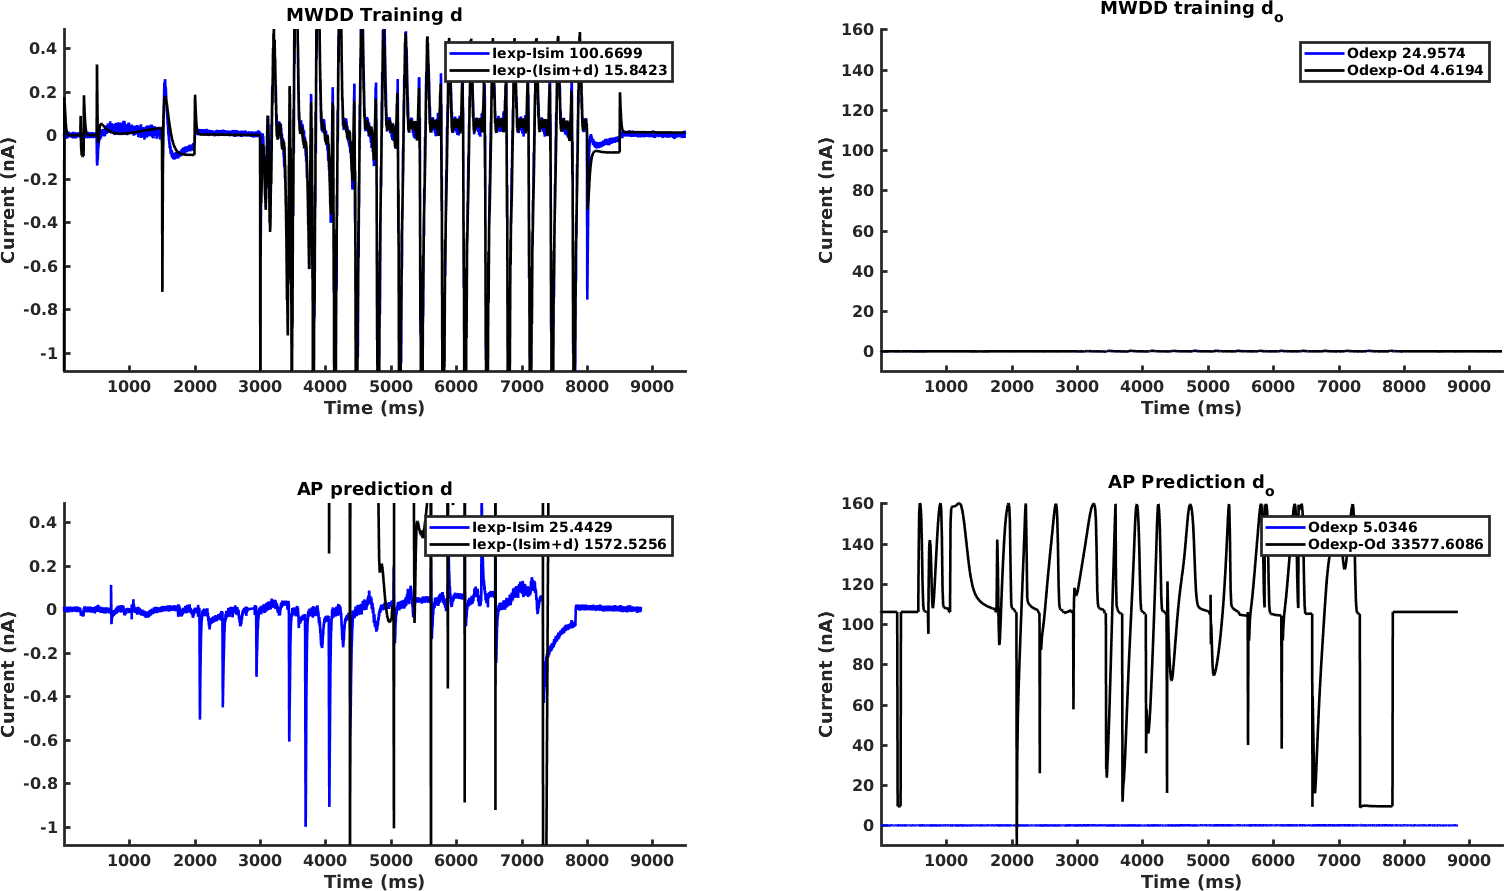
\includegraphics[scale=0.42]{Figures/StepwiseLM_MWDD_AP_full_discrepancy.png}
\caption{\textbf{Linear model of discrepancy constructed using StepwiseLM from the MWDD protocol.} These models of $d$ (left) and $d_o$ (right) were constructed using StepwiseLM on the entire MWDD trace (top), starting with all linearly independent predictors. The root mean square errors between the simulated and predicted traces are shown in the legends. } 
\label{Fig_StepwiseLM_MWDD_AP_full_discrepancy}
\end{center}
\end{figure}

\begin{figure}[hb]
\begin{center}
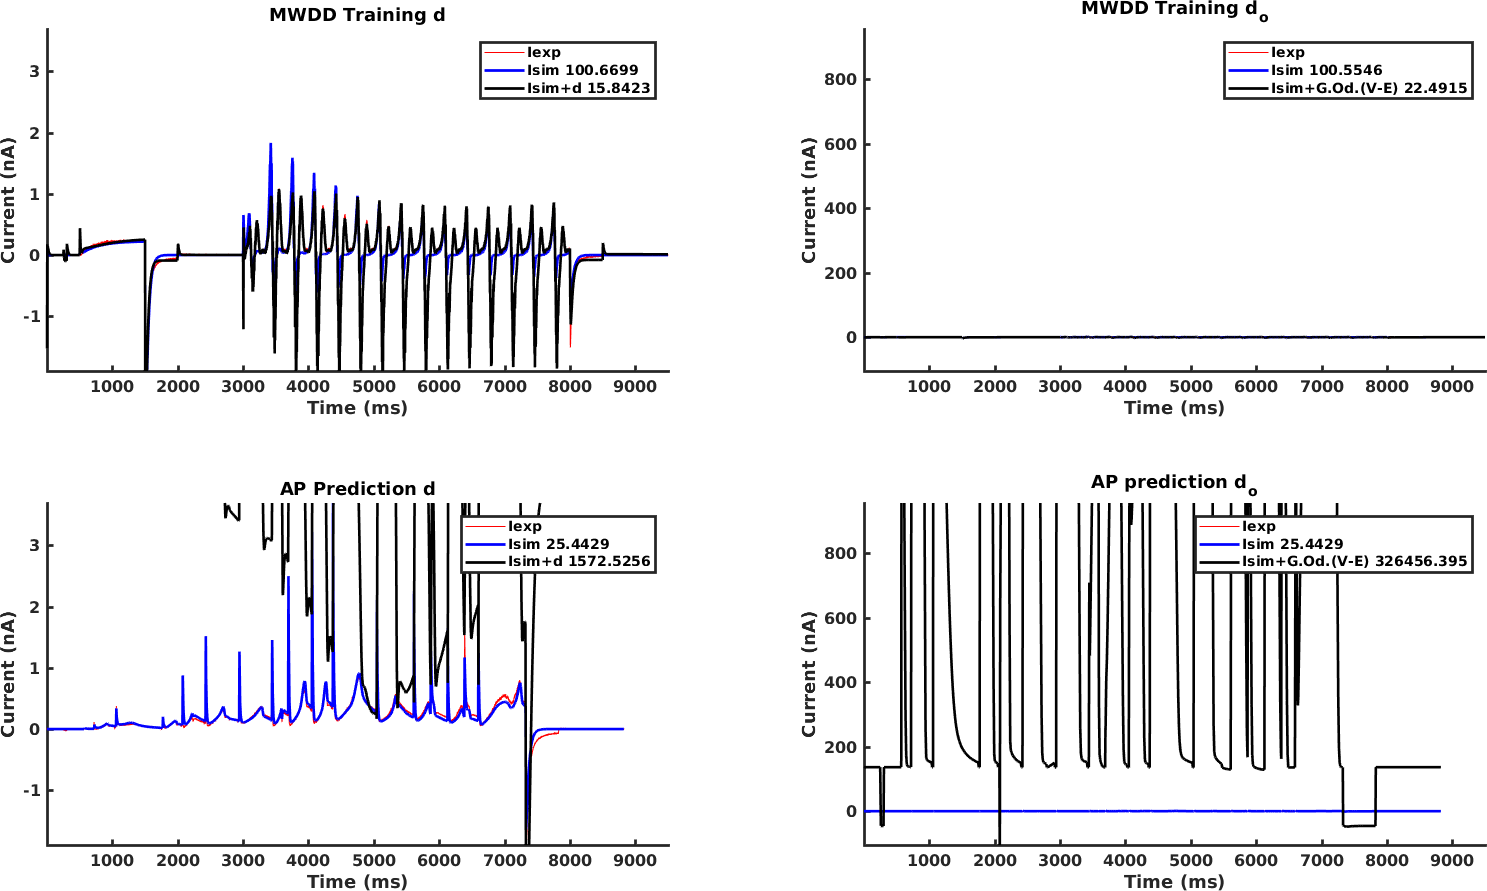
\includegraphics[scale=0.42]{Figures/StepwiseLM_MWDD_AP_full_currents.png}
\caption{\textbf{Corrected currents using a linear model of discrepancy constructed using StepwiseLM from the MWDD protocol.} The models of $d$ (left) and $d_o$ (right) in Fig. ~\ref{Fig_StepwiseLM_MWDD_AP_full_discrepancy} have been incorporated into the simulation (blue line), giving a revised prediction for the MWDD and AP protocols (black line). The sum of squared errors between the models and the data are shown in the legend.}
\label{Fig_StepwiseLM_MWDD_AP_full_currents}
\end{center}
\end{figure}

\clearpage

\begin{figure}[t]
\begin{center}
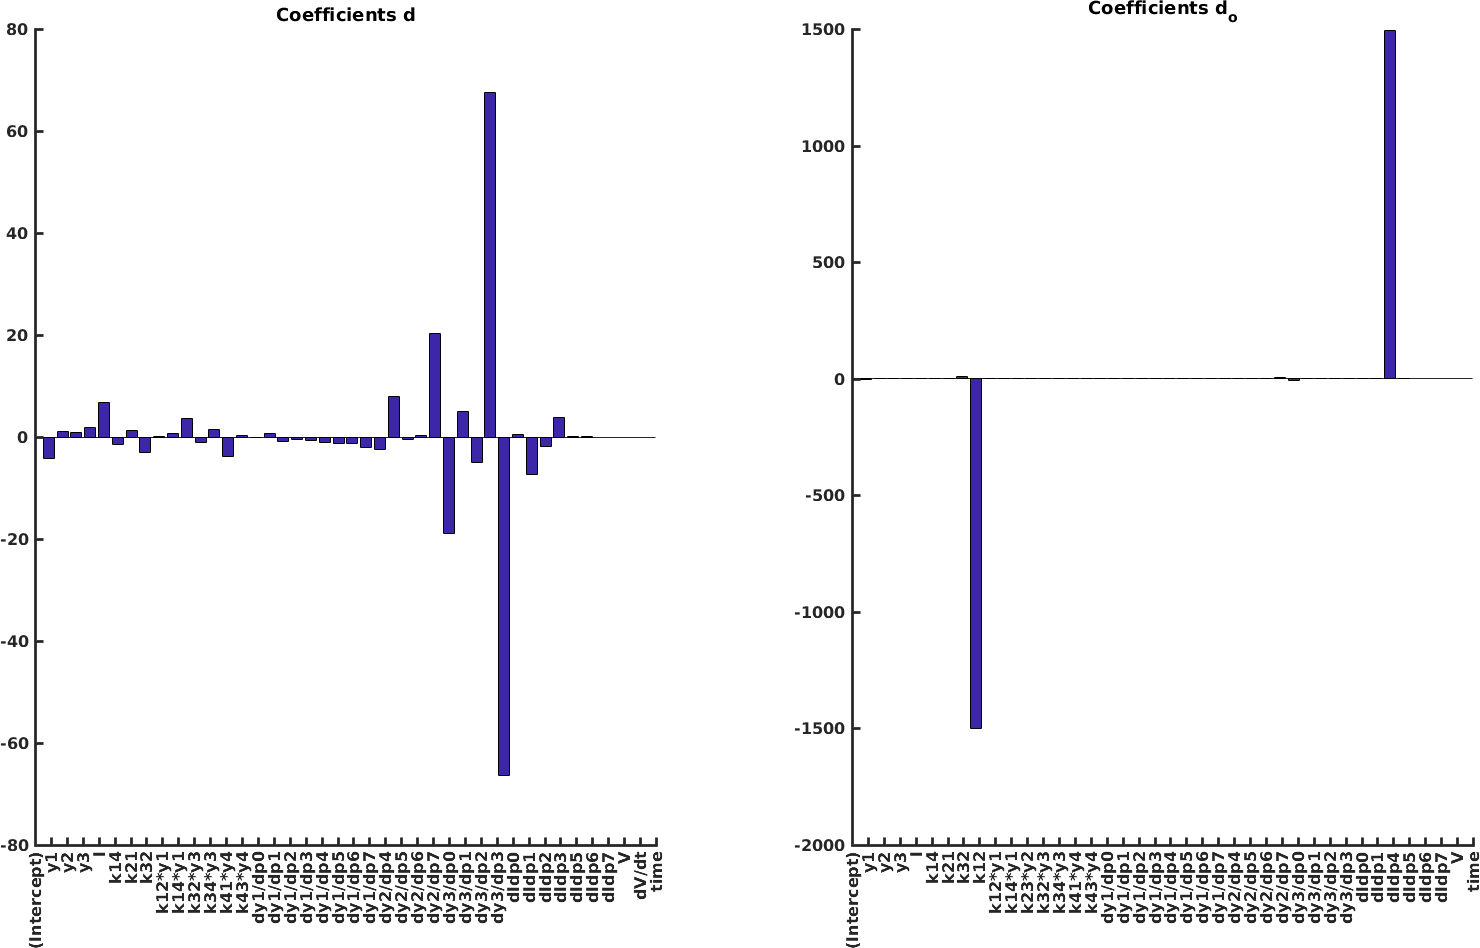
\includegraphics[scale=0.42]{Figures/StepwiseLM_MWDD_AP_full_coefficients.png}
\caption{\textbf{Coefficients in the linear model of discrepancy constructed using StepwiseLM from the MWDD protocol.} This plot shows the included parameters and coefficients for the model produced by StepwiseLM shown in Fig.~\ref{Fig_StepwiseLM_MWDD_AP_full_discrepancy} and Fig.~\ref{Fig_StepwiseLM_MWDD_AP_full_currents}. Coefficients for $d$ are shown on the left, and coefficients for $d_o$ are shown on the right.} 
\label{Fig_StepwiseLM_MWDD_AP_full_coefficients}
\end{center}
\end{figure}

\clearpage

\begin{figure}[t]
\begin{center}
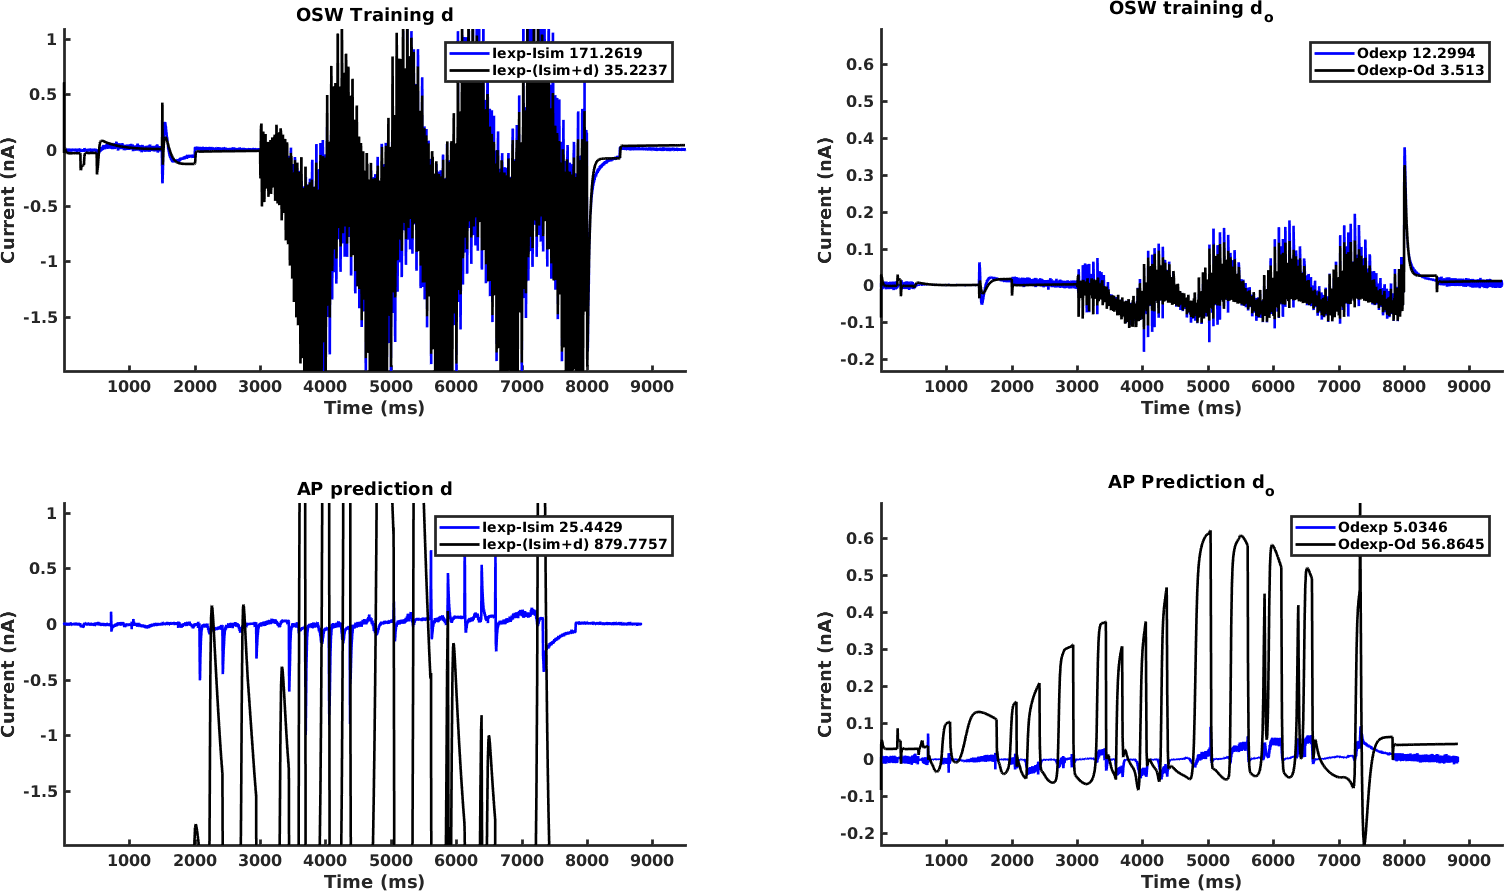
\includegraphics[scale=0.42]{Figures/StepwiseLM_OSW_AP_full_discrepancy.png}
\caption{\textbf{Linear model of discrepancy constructed using StepwiseLM from the OSW protocol.} These models of $d$ (left) and $d_o$ (right) were constructed using StepwiseLM on the entire OSW trace (top), starting with all linearly independent predictors. The root mean square errors between the simulated and predicted traces are shown in the legends. } 
\label{Fig_StepwiseLM_OSW_AP_full_discrepancy}
\end{center}
\end{figure}

\begin{figure}[hb]
\begin{center}
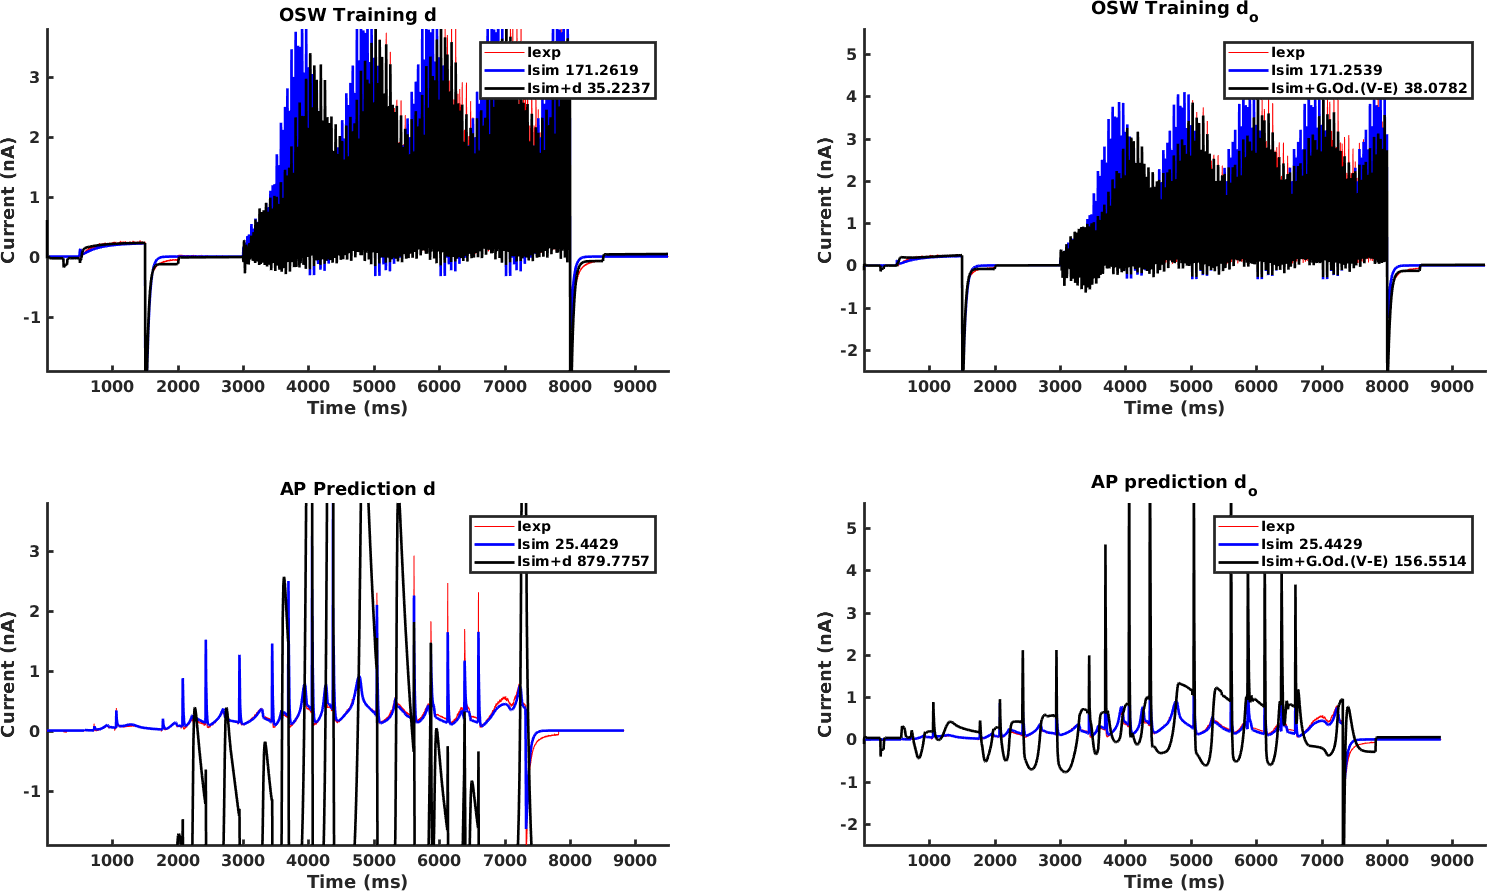
\includegraphics[scale=0.42]{Figures/StepwiseLM_OSW_AP_full_currents.png}
\caption{\textbf{Corrected currents using a linear model of discrepancy constructed using StepwiseLM from the OSW protocol.} The models of $d$ (left) and $d_o$ (right) in Fig. ~\ref{Fig_StepwiseLM_OSW_AP_full_discrepancy} have been incorporated into the simulation (blue line), giving a revised prediction for the OSW and AP protocols (black line). The sum of squared errors between the models and the data are shown in the legend.}
\label{Fig_StepwiseLM_OSW_AP_full_currents}
\end{center}
\end{figure}

\clearpage

\begin{figure}[t]
\begin{center}
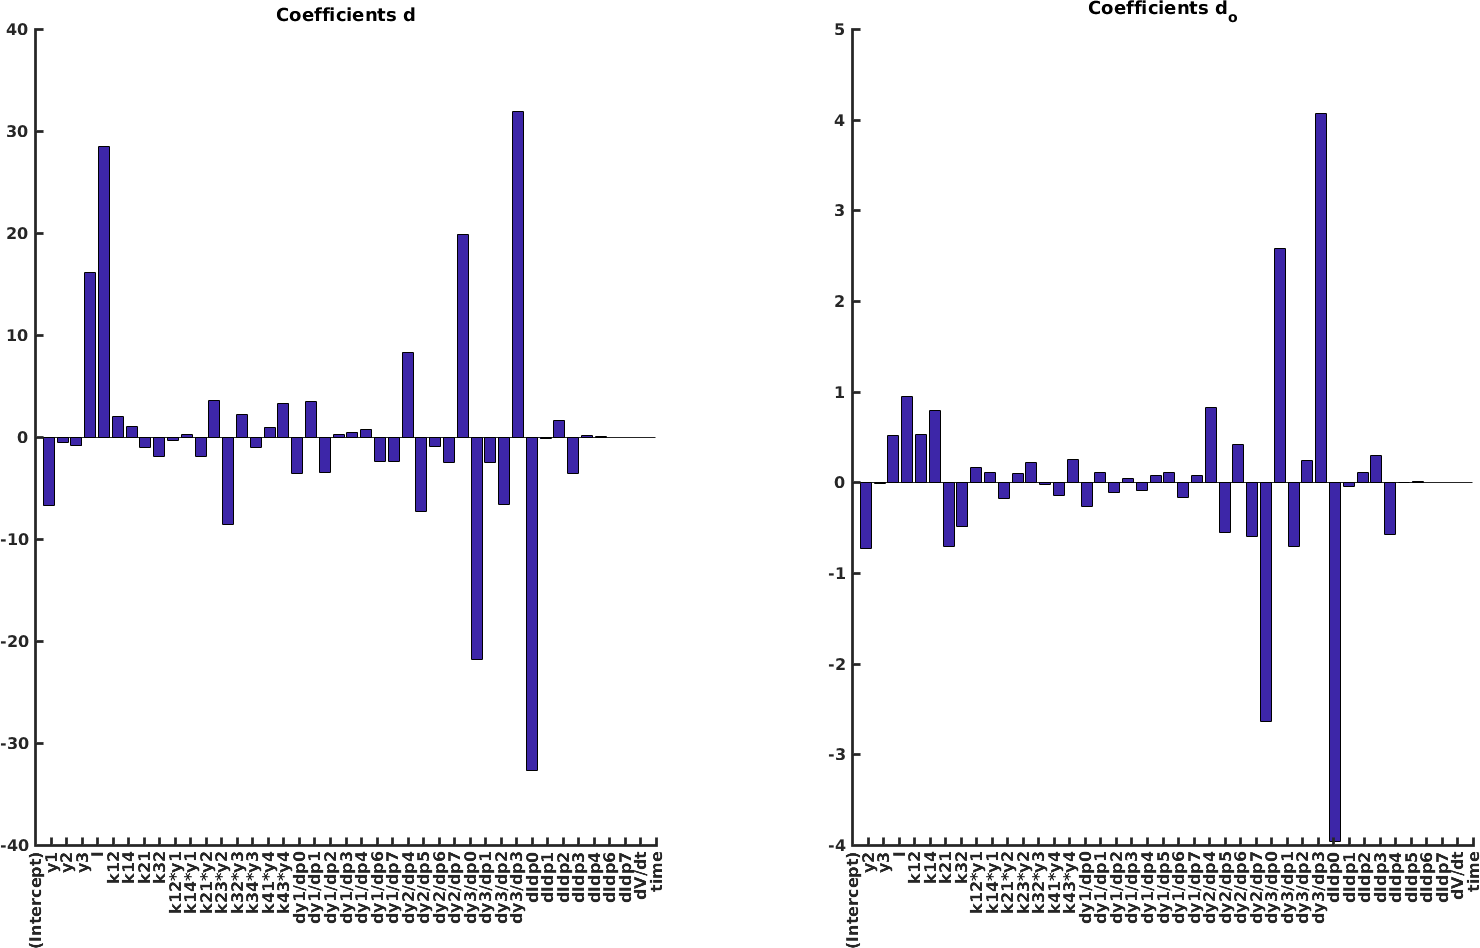
\includegraphics[scale=0.42]{Figures/StepwiseLM_OSW_AP_full_coefficients.png}
\caption{\textbf{Coefficients in the linear model of discrepancy constructed using StepwiseLM from the OSW protocol.} This plot shows the included parameters and coefficients for the model produced by StepwiseLM shown in Fig.~\ref{Fig_StepwiseLM_OSW_AP_full_discrepancy} and Fig.~\ref{Fig_StepwiseLM_OSW_AP_full_currents}. Coefficients for $d$ are shown on the left, and coefficients for $d_o$ are shown on the right.} 
\label{Fig_StepwiseLM_OSW_AP_full_coefficients}
\end{center}
\end{figure}

\clearpage

\begin{figure}[t]
\begin{center}
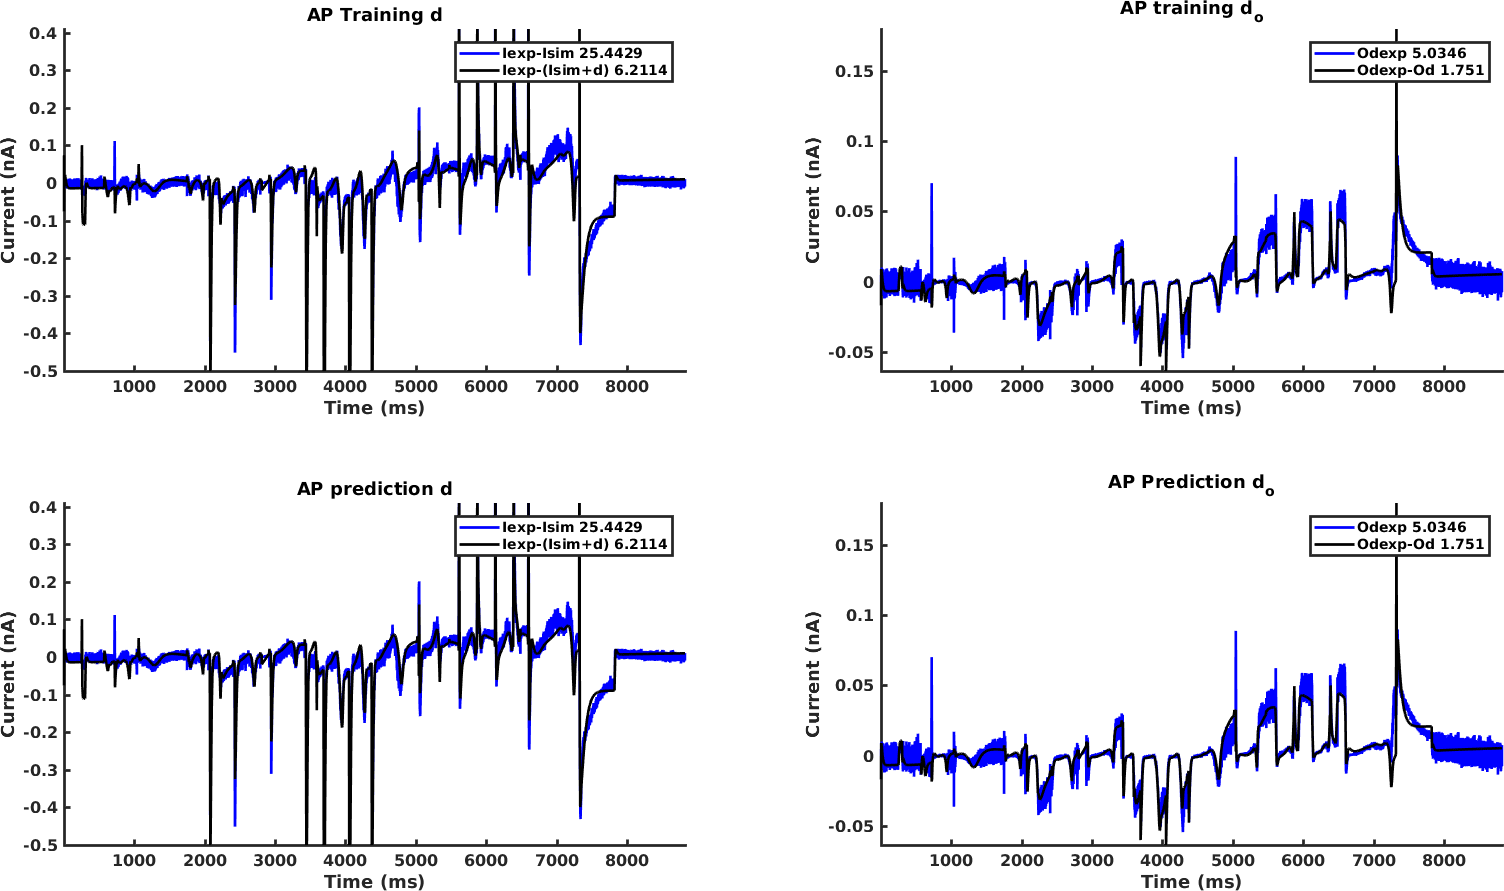
\includegraphics[scale=0.42]{Figures/StepwiseLM_AP_AP_full_discrepancy.png}
\caption{\textbf{Linear model of discrepancy constructed using StepwiseLM from the AP protocol.} These models of $d$ (left) and $d_o$ (right) were constructed using StepwiseLM on the entire AP trace (top), starting with all linearly independent predictors. The root mean square errors between the simulated and predicted traces are shown in the legends. Note that the top and bottom rows of this figure are the same. } 
\label{Fig_StepwiseLM_AP_AP_full_discrepancy}
\end{center}
\end{figure}

\begin{figure}[hb]
\begin{center}
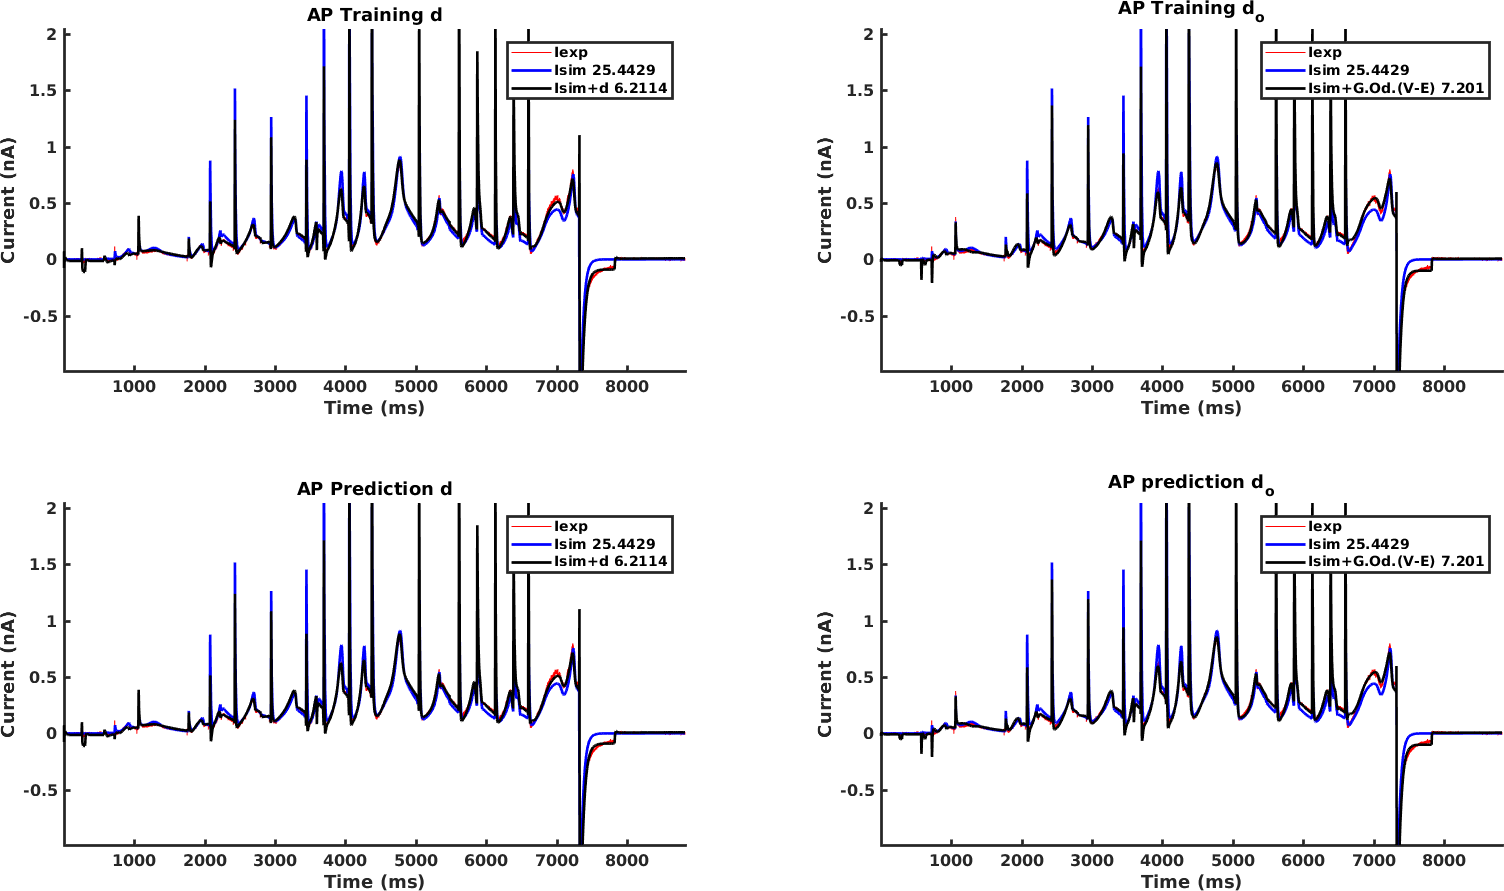
\includegraphics[scale=0.42]{Figures/StepwiseLM_AP_AP_full_currents.png}
\caption{\textbf{Corrected currents using a linear model of discrepancy constructed using StepwiseLM from the OSW protocol.} The models of $d$ (left) and $d_o$ (right) in Fig. ~\ref{Fig_StepwiseLM_AP_AP_full_discrepancy} have been incorporated into the simulation (blue line), giving a revised prediction for the AP protocol (black line). The sum of squared errors between the models and the data are shown in the legend.Note that the top and bottom rows of this figure are the same.}
\label{Fig_StepwiseLM_AP_AP_full_currents}
\end{center}
\end{figure}

\clearpage

\begin{figure}[t]
\begin{center}
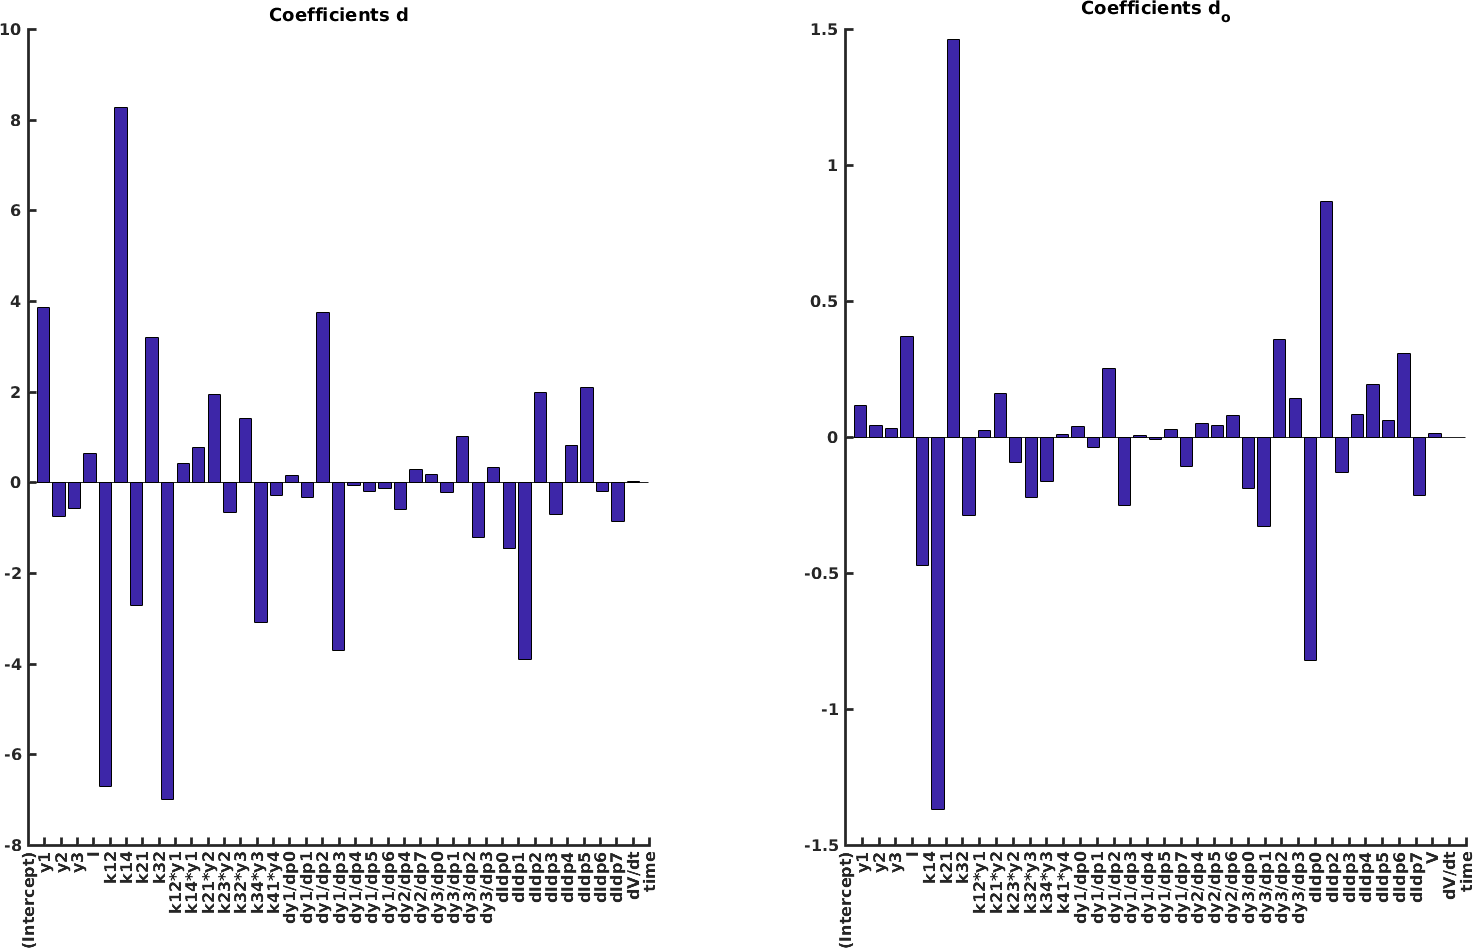
\includegraphics[scale=0.42]{Figures/StepwiseLM_AP_AP_full_coefficients.png}
\caption{\textbf{Coefficients in the linear model of discrepancy constructed using StepwiseLM from the AP protocol.} This plot shows the included parameters and coefficients for the model produced by StepwiseLM shown in Fig.~\ref{Fig_StepwiseLM_AP_AP_full_discrepancy} and Fig.~\ref{Fig_StepwiseLM_AP_AP_full_currents}. Coefficients for $d$ are shown on the left, and coefficients for $d_o$ are shown on the right.} 
\label{Fig_StepwiseLM_AP_AP_full_coefficients}
\end{center}
\end{figure}

\clearpage

\subsection{Artificial Data}
Given the disappointing results in Sections \ref{SubSec_Lasso_Discrepancy} and \ref{SubSec_StepwiseLM_Discrepancy} above, we performed a set of test studies to determine how well the methods could be expected to perform under these circumstances. The first test was to use the AP trace for training, thereby determining an `optimal' model - this approach places a bound on the quality of the fit that should be expected from the method applied - it is constructing a model using the prediction data as shown above. 

The second method we used to determine how effective the methods were likely to be was to generate artificial data. In this approach, we assume that our central hypothesis is true and that the discrepancy between the model and the data can be represented by a linear sum of the model-derived predictors in Section~\ref{SubSec_Predictors}. `Discrepancies' are generated by firstly choosing a random number of $n$ predictors between 1 and 20, and then randomly selecting $n$ predictors. These predictors are then summed with a constant linear coefficient so that the magnitude is comparable to the magnitude of the $d$ trace. Finally, Gaussian noise with mean 0 and standard deviation from the first 1000 time points in the $d$ trace is applied. The process was repeated in the absence of noise. Two examples constructed using LASSO are shown in Figs.~\ref{Fig_LassoArtificialExample}. We repeated this process 20 times and then recorded the relationship between the number of parameters in the model and the MSE between the true model's coefficients and the fitted model's coefficients. Non-included predictors were treated as having a coefficient value of zero. The results are shown in Fig.~\ref{Fig_BatchArtificialFits}, showing that the more parameters are included in the target model, the less likely the model is to be correct. Consequently, large models produced through this fitting method are unlikely to be reliable, consistent with the results shown when using the experimental data in the previous section.

\begin{figure}[t]
\begin{center}
\includegraphics[scale=0.42]{Figures/LassoArtificialExample1_TrainingVsPrediction.png} \hspace{1cm}
\includegraphics[scale=0.21]{Figures/LassoArtificialExample1_Coeffs.png} \newline \newline
\includegraphics[scale=0.42]{Figures/LassoArtificialExample2_TrainingVsPrediction.png} \hspace{1cm}
\includegraphics[scale=0.21]{Figures/LassoArtificialExample2_Coeffs.png}
\caption{\textbf{Example fits using LASSO to artificial data}. The fit of the model to the artificial data is shown on the left, and the coeffcicients in the constructed model and the original model are shown on the right.} 
\label{Fig_LassoArtificialExample}
\end{center}
\end{figure}

\begin{figure}[bt]
\begin{center}
\includegraphics[scale=0.42]{Figures/BatchFitToData.png}
\caption{\textbf{Effectiveness of LASSO and StepwiseLM at recovering artificial data}. The MSE between the original coefficients constructing the artificial model, and the coefficients of the fitted linear model is shown on the y axis, and the number of parameters included in the artificial model is shown on the x-axis. The left panel shows the results for LASSO and the right panel shows the results for StepwiseLM.} 
\label{Fig_BatchArtificialFits}
\end{center}
\end{figure}

\subsection{Conclusions}

The LASSO method tended to produce very small models, particularly for $d_o$. These models were not capable of predicting the discrepancy in the AP trace, even though the analysis in Fig.~\ref{Fig_BatchArtificialFits} suggests that they ought to be relatively reliable if they were detecting a real signal. The fact that these models are unreliable is consistent with them being inaccurate. It is notable that the difference between the folds in most cases is large relative to the MSE, which would suggest that the model is not particularly effective for prediction even within the training data, and explains why very small models tended to be chosen - the LASSO method could not conclude that the larger model with the smallest overall MSE was definitely better than a sparse model. This shows the value of K-fold cross-validation on the training data in any future application of similar methods. Conversely, StepwiseLM tended to produce large linear models which are likely to be untrustworthy based on the simulated data examples in Fig.~\ref{Fig_BatchArtificialFits}. Their lack of predictive function supports this view. We also note that the small discrepancy between the original parameterized model and the experimental data does not seem to be the source of the problem - in the cases where alternative protocols (EP, MWDD, OSW) were used to fit the linear model, the result tended to be worse than for the SW protocol.

It is striking that the two different methods, over multiple different datasets, are very rarely consistent in the predictors they include in the model, either between datasets or between methods. This finding further indicates that a true structural source for the discrepancy is not being successfully identified, as if a source of error were to exist amongst these variables it would be expected to be consistently included. It is also instructive to note that in the two cases where the model was constructed from the prediction data (AP protocol), the error could be reduced to a magnitude comparable to that in the SW protocol data prior to fitting. This is encouraging at first sight. However, the two constructed models are completely different and both very large. Furthermore, the error is much lower in StepwiseLM than LASSO, which may suggest a better model, or alternatively overfititng due to the lack of K-fold cross validation.

Based on the results shown above, we conclude that straightforward linear regression on predictors derived from the HH model equations is unlikely to be an effective method for predicting discrepancy. Unfortunately, this assertion is difficult to prove conclusively as we do not know the structure of the experimental data. Furthermore, in the trivial case where the discrepancy is included in the predictors then the method should always work. Taking these two facts together, we see that any proof without knowledge of how the data ought to behave is likely to be impossible. As mentioned in Section~\ref{Sec_FutureWork}, an approach based on simulations of different model structures may yield insights, but the results presented above suggest that the effort may be better spent elsewhere if practical application of the method within the CiPA framework is desired. 

\section{Parameter Fits Using Alternate Protocols}

\section{Discrepancy Between Alternate Model Structures}\label{Sec_ModelDiscrepancy}

\section{Future Work}\label{Sec_FutureWork}

\section{Acknowledgements}
The authors would like to thank Dr.~Simon Preston and Dr.~Theo Kypraios (University of Nottingham) for useful discussions on LASSO and K-fold cross validation; Dr.~Kylie Beattie (GlaxoSmithKline) for help with data processing and implementation of alternate pacing protocols; and Dr.~Michael Clerx and Dr.~Sanmitra Ghosh (University of Oxford) for useful discussions on Hodgkin-Huxley models and model discrepancy. This study was funded by a Wellcome Trust and Royal Society Sir Henry Dale Fellowship to Dr.~Gary R.~Mirams (grant number 101222/Z/13/Z).

\bibliographystyle{plain}
\bibliography{Bibliography}

\end{document}
